% answers.tex —— 2015 年·浙江卷·文科 · 参考答案与详细解析片段
% 由 tools/generate_projects.py 依来源总账自 2015/2015_数学真题_浙江文_试题.md + 2015/2015_数学真题_浙江文_解析正文.md + 2015/2015_数学真题_浙江文_答案要点.md 生成，勿手改（改源 MD 后重跑）

\begin{gktip}
固定原卷不附参考答案（证据等级 D）；以下推导由项目独立完成，并经独立角色盲核，不作为官方解析。
\end{gktip}

\begin{answer}
\gksolhead{1}{集合运算}

\textbf{题目}：

已知集合 \(P=\{x\mid x^2-2x\geqslant 3\}\)，\(Q=\{x\mid 2<x<4\}\)，则 \(P\cap Q=\)（　）

(A) \([3,4)\)　(B) \((2,3]\)　(C) \((-1,2)\)　(D) \((-1,3]\)

\Needspace{4\baselineskip}
\textbf{解析}

\Needspace{5\baselineskip}
由 \(x^2-2x\geqslant3\) 得 \(x^2-2x-3\geqslant0\)，即 \((x-3)(x+1)\geqslant0\)，故
\nopagebreak[4]
\[
P=(-\infty,-1]\cup[3,+\infty).
\]
\Needspace{5\baselineskip}
又 \(Q=(2,4)\)，求交得
\nopagebreak[4]
\[
P\cap Q=[3,4).
\]

故选 (A)。

（验证：取 \(x=3.5\in Q\)，\(3.5^2-7=5.25\geqslant3\)，在 \(P\) 中；取 \(x=2.5\in Q\)，\(2.5^2-5=-0.75<3\)，不在 \(P\) 中；端点 \(x=3\) 满足等号，属于 \(P\)。）

\gkanswer{答案：A}

\end{answer}
\begin{answer}
\gksolhead{2}{三视图与体积}

\textbf{题目}：

某几何体的三视图如图所示（单位：\(\mathrm{cm}\)），则该几何体的体积是（　）
\nopagebreak[4]
\begin{center}% f2015zjw_q02_views.tex — 2015 年高考数学·浙江卷·文科 第 2 题（三视图）
%
% 【来源】`.work/phase3-b18/source/2015浙江文.pdf`（SHA-256
%   a0e49283fb3d086029ec3c96de7e96cc6118365378ea0a24273c6f58285ec977），
%   第 1 页（合订本页 991）；内容对象 5。逐路径实测见
%   `.work/phase3-b18/figure-inventory.md`。
%
% 【坐标口径】源 PDF 用户空间（原点左下、y 向上）。本图本地坐标
%   (x, y) = (x_page − 145.498, y_page − 395.595)，1 单位 = 1 TeX pt。
%   路径坐标逐点照录内容流（含三次贝塞尔控制点）。
%
% 元素计数：30 条路径（三视图轮廓/对角线/尺寸线/箭头）＋7 个标签
\begin{tikzpicture}[x=1pt, y=1pt,
    every node/.style={inner sep=0pt, font=\fontsize{10.5pt}{12.6pt}\selectfont}]
  \draw[line width=0.398pt] (0.0000,9.3547)   -- (62.3630,71.7177);
  \draw[line width=0.398pt] (0.0000,71.7180)   -- (62.3630,9.3550);
  \draw[line width=0.398pt] (0.0000,165.2630)   -- (62.3630,165.2630);
  \draw[line width=0.398pt] (93.5450,165.2630)   -- (155.9080,165.2630);
  \draw[line width=0.398pt] (0.0000,6.2363)   -- (0.0000,0.0003);
  \draw[line width=0.398pt] (62.3633,6.2363)   -- (62.3633,0.0003);
  \draw[line width=0.398pt] (65.4817,9.3547)   -- (71.7177,9.3547);
  \draw[line width=0.398pt] (65.4817,71.7180)   -- (71.7177,71.7180);
  \draw[line width=0.398pt] (65.4817,102.8996)   -- (71.7177,102.8996);
  \draw[line width=0.398pt] (65.4817,165.2630)   -- (71.7177,165.2630);
  \draw[line width=0.398pt] (65.4817,227.6263)   -- (71.7177,227.6263);
  \draw[line width=0.398pt] (24.9454,3.1184)   -- (3.5864,3.1184);
  \fill[line width=1.0pt] (0.0000,3.1184)   .. controls (1.0630,2.9194) and (2.7900,2.3214) .. (3.9850,1.6244)   -- (3.9850,4.6124)   .. controls (2.7900,3.9154) and (1.0630,3.3174) .. (0.0000,3.1184);
  \draw[line width=0.398pt] (68.5995,34.3001)   -- (68.5995,12.9411);
  \fill[line width=1.0pt] (68.5996,9.3547)   .. controls (68.7986,10.4177) and (69.3966,12.1447) .. (70.0936,13.3397)   -- (67.1056,13.3397)   .. controls (67.8026,12.1447) and (68.4006,10.4177) .. (68.5996,9.3547);
  \draw[line width=0.398pt] (68.5995,46.7725)   -- (68.5995,68.1315);
  \fill[line width=1.0pt] (68.5996,71.7179)   .. controls (68.4006,70.6549) and (67.8026,68.9279) .. (67.1056,67.7329)   -- (70.0936,67.7329)   .. controls (69.3966,68.9279) and (68.7986,70.6549) .. (68.5996,71.7179);
  \draw[line width=0.398pt] (68.5995,127.8451)   -- (68.5995,106.4861);
  \fill[line width=1.0pt] (68.5996,102.8997)   .. controls (68.7986,103.9627) and (69.3966,105.6897) .. (70.0936,106.8847)   -- (67.1056,106.8847)   .. controls (67.8026,105.6897) and (68.4006,103.9627) .. (68.5996,102.8997);
  \draw[line width=0.398pt] (68.5995,140.3175)   -- (68.5995,161.6765);
  \fill[line width=1.0pt] (68.5996,165.2629)   .. controls (68.4006,164.1999) and (67.8026,162.4729) .. (67.1056,161.2779)   -- (70.0936,161.2779)   .. controls (69.3966,162.4729) and (68.7986,164.1999) .. (68.5996,165.2629);
  \draw[line width=0.398pt] (68.5995,190.2084)   -- (68.5995,168.8494);
  \fill[line width=1.0pt] (68.5996,165.2630)   .. controls (68.7986,166.3260) and (69.3966,168.0530) .. (70.0936,169.2480)   -- (67.1056,169.2480)   .. controls (67.8026,168.0530) and (68.4006,166.3260) .. (68.5996,165.2630);
  \draw[line width=0.398pt] (68.5995,202.6809)   -- (68.5995,224.0399);
  \fill[line width=1.0pt] (68.5996,227.6263)   .. controls (68.4006,226.5633) and (67.8026,224.8363) .. (67.1056,223.6413)   -- (70.0936,223.6413)   .. controls (69.3966,224.8363) and (68.7986,226.5633) .. (68.5996,227.6263);
  \draw[line width=0.398pt] (37.4179,3.1184)   -- (58.7769,3.1184);
  \fill[line width=1.0pt] (62.3633,3.1184)   .. controls (61.3003,3.3174) and (59.5733,3.9154) .. (58.3783,4.6124)   -- (58.3783,1.6244)   .. controls (59.5733,2.3214) and (61.3003,2.9194) .. (62.3633,3.1184);
  \draw[line width=0.398pt] (0.0000,9.3547)   -- (0.0000,71.7177)   -- (62.3630,71.7177)   -- (62.3630,9.3547)   -- cycle;
  \draw[line width=0.398pt] (0.0000,102.8996)   -- (62.3630,102.8996)   -- (62.3630,165.2626)   -- (31.1820,227.6266)   -- (0.0000,165.2626)   -- cycle;
  \draw[line width=0.398pt] (93.5450,102.8996)   -- (155.9080,102.8996)   -- (155.9080,165.2626)   -- (124.7270,227.6266)   -- (93.5450,165.2626)   -- cycle;

  \node[anchor=center] at (31.152,87.945) {正视图};  % 源中心 (176.65,483.54)
  \node[anchor=center] at (124.752,87.945) {侧视图};  % 源中心 (270.25,483.54)
  \node[anchor=center] at (31.152,-10.255) {俯视图};  % 源中心 (176.65,385.34)
  \node[anchor=center] at (68.602,195.695) {$2$};  % 源中心 (214.10,591.29)
  \node[anchor=center] at (68.602,133.345) {$2$};  % 源中心 (214.10,528.94)
  \node[anchor=center] at (68.602,39.745) {$2$};  % 源中心 (214.10,435.34)
  \node[anchor=center] at (31.202,2.345) {$2$};  % 源中心 (176.70,397.94)

\end{tikzpicture}
%
% 【自验结果】
%   探针：latexmk -pdfxe（待跑）。
\end{center}
\nopagebreak[4]
(A) \(8\,\mathrm{cm}^3\)　(B) \(12\,\mathrm{cm}^3\)　(C) \(\dfrac{32}{3}\,\mathrm{cm}^3\)　(D) \(\dfrac{40}{3}\,\mathrm{cm}^3\)

\Needspace{4\baselineskip}
\textbf{解析}

由三视图可知，该几何体下部是棱长为 \(2\) 的正方体，上部是底面为 \(2\times2\)、高为 \(2\) 的四棱锥（俯视图中的对角线即四棱锥的四条侧棱在水平面上的投影）。

\Needspace{5\baselineskip}
下部体积
\nopagebreak[4]
\[
V_1=2^3=8.
\]
\Needspace{5\baselineskip}
上部四棱锥体积
\nopagebreak[4]
\[
V_2=\frac13\cdot2^2\cdot2=\frac83.
\]
\Needspace{5\baselineskip}
故几何体体积
\nopagebreak[4]
\[
V=V_1+V_2=8+\frac83=\frac{32}{3}\ \left(\mathrm{cm}^3\right).
\]

故选 (C)。

（验证：正视图与侧视图均为「边长 2 的正方形上加高 2 的等腰三角形」，与「正方体＋四棱锥」的投影一致；俯视图为带两条对角线的正方形，对角线交点即锥顶投影。）

\gkanswer{答案：C}

\end{answer}
\begin{answer}
\gksolhead{3}{充分必要条件}

\textbf{题目}：

设 \(a\)，\(b\) 是实数，则“\(a+b>0\)”是“\(ab>0\)”的（　）

(A) 充分不必要条件　(B) 必要不充分条件　(C) 充分必要条件　(D) 既不充分也不必要条件

\Needspace{4\baselineskip}
\textbf{解析}

取 \(a=3\)，\(b=-1\)：\(a+b=2>0\)，但 \(ab=-3<0\)，故「\(a+b>0\)」不是「\(ab>0\)」的充分条件。

取 \(a=b=-1\)：\(ab=1>0\)，但 \(a+b=-2<0\)，故「\(a+b>0\)」也不是「\(ab>0\)」的必要条件。

因此「\(a+b>0\)」是「\(ab>0\)」的既不充分也不必要条件。

故选 (D)。

（验证：两个反例分别否定了充分性与必要性，方向完整。）

\gkanswer{答案：D}

\end{answer}
\begin{answer}
\gksolhead{4}{空间线面关系}

\textbf{题目}：

设 \(\alpha\)，\(\beta\) 是两个不同的平面，\(l\)，\(m\) 是两条不同的直线，且 \(l\subset\alpha\)，\(m\subset\beta\)。（　）

(A) 若 \(l\perp\beta\)，则 \(\alpha\perp\beta\)　(B) 若 \(\alpha\perp\beta\)，则 \(l\perp m\)　(C) 若 \(l\parallel\beta\)，则 \(\alpha\parallel\beta\)　(D) 若 \(\alpha\parallel\beta\)，则 \(l\parallel m\)

\Needspace{4\baselineskip}
\textbf{解析}

(A) 若 \(l\perp\beta\)，且 \(l\subset\alpha\)，则由面面垂直的判定定理，\(\alpha\perp\beta\)。正确。

(B) 若 \(\alpha\perp\beta\)，\(l\subset\alpha\)，\(m\subset\beta\)，则 \(l\) 与 \(m\) 可以平行、相交或异面，不一定垂直。错误。

(C) 若 \(l\parallel\beta\)，\(l\subset\alpha\)，则 \(\alpha\) 与 \(\beta\) 可能相交，不一定平行。错误。

(D) 若 \(\alpha\parallel\beta\)，\(l\subset\alpha\)，\(m\subset\beta\)，则 \(l\) 与 \(m\) 可能异面，不一定平行。错误。

故选 (A)。

（验证：以正方体为模型，(B)(C)(D) 均可各举一反例；只有 (A) 由判定定理直接成立。）

\gkanswer{答案：A}

\end{answer}
\begin{answer}
\gksolhead{5}{函数图象}

\textbf{题目}：

函数 \(f(x)=\left(x-\dfrac{1}{x}\right)\cos x\)（\(-\pi\leqslant x\leqslant\pi\) 且 \(x\neq0\)）的图象可能为（　）
\nopagebreak[4]
\begin{center}% f2015zjw_q05_graphs.tex — 2015 年高考数学·浙江卷·文科 第 5 题（四函数图象选项）
%
% 【来源】`.work/phase3-b18/source/2015浙江文.pdf`（SHA-256
%   a0e49283fb3d086029ec3c96de7e96cc6118365378ea0a24273c6f58285ec977），
%   第 1 页（合订本页 991）；内容对象 5。逐路径实测见
%   `.work/phase3-b18/figure-inventory.md`。
%
% 【坐标口径】源 PDF 用户空间（原点左下、y 向上）。本图本地坐标
%   (x, y) = (x_page − 87.166, y_page − 56.446)，1 单位 = 1 TeX pt。
%   路径坐标逐点照录内容流（含三次贝塞尔控制点）。
%
% 元素计数：32 条路径（4 面板 × 8：x/y 轴＋箭头＋2 虚线＋2 曲线段）＋20 个标签
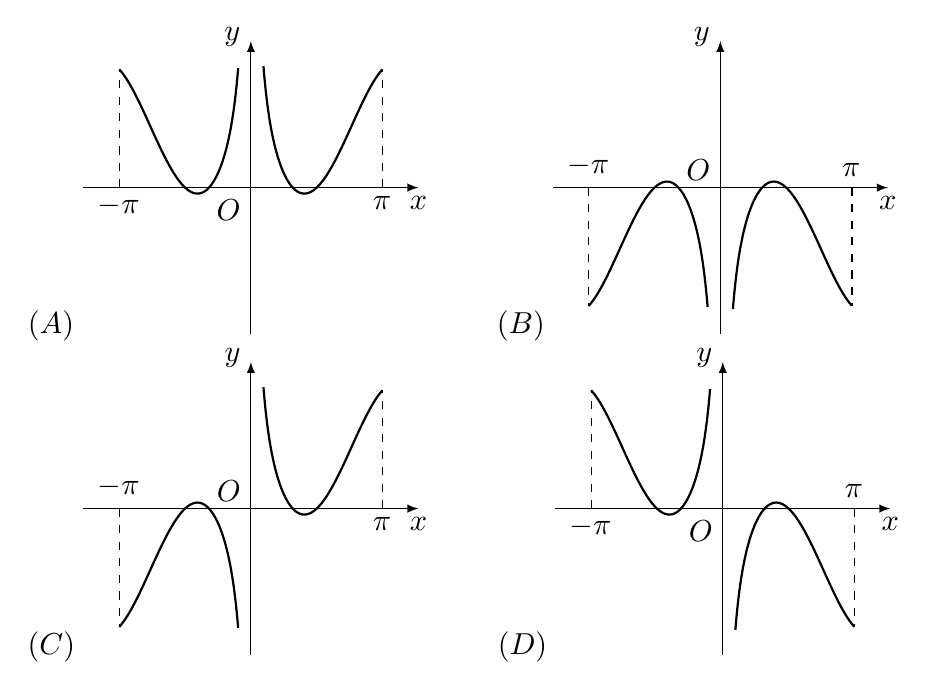
\begin{tikzpicture}[x=1pt, y=1pt,
    every node/.style={inner sep=0pt, font=\fontsize{10.5pt}{12.6pt}\selectfont}]
  \begin{scope}[shift={(0.000,0.000)}]
  \draw[line width=0.398pt] (-0.0004,52.9800)   -- (117.5096,52.9800);
  \fill[line width=1.0pt] (121.0963,52.9800)   .. controls (120.0333,53.1790) and (118.3063,53.7770) .. (117.1113,54.4740)   -- (117.1113,51.4860)   .. controls (118.3063,52.1830) and (120.0333,52.7810) .. (121.0963,52.9800);
  \draw[line width=0.398pt] (60.5480,0.0002)   -- (60.5480,102.3732);
  \fill[line width=1.0pt] (60.5480,105.9598)   .. controls (60.3490,104.8968) and (59.7510,103.1698) .. (59.0540,101.9748)   -- (62.0420,101.9748)   .. controls (61.3450,103.1698) and (60.7470,104.8968) .. (60.5480,105.9598);
  \draw[line width=0.398pt, dash pattern=on 2.989pt off 2.989pt, dash phase=0.0pt] (12.9935,52.9800)   -- (12.9935,95.7160);
  \draw[line width=0.398pt, dash pattern=on 2.989pt off 2.989pt, dash phase=0.0pt] (108.1025,52.9800)   -- (108.1025,95.7160);
  \draw[line width=0.797pt] (12.9935,95.7154)   .. controls (12.9935,95.7154) and (13.0975,95.5994) .. (13.1375,95.5544)   .. controls (13.1775,95.5084) and (13.2405,95.4364) .. (13.2805,95.3904)   .. controls (13.3205,95.3444) and (13.3845,95.2684) .. (13.4245,95.2214)   .. controls (13.4645,95.1744) and (13.5285,95.0994) .. (13.5685,95.0504)   .. controls (13.6085,95.0024) and (13.6715,94.9244) .. (13.7115,94.8744)   .. controls (13.7515,94.8254) and (13.8155,94.7454) .. (13.8555,94.6954)   .. controls (13.8955,94.6444) and (13.9595,94.5634) .. (13.9995,94.5124)   .. controls (14.0395,94.4614) and (14.1025,94.3784) .. (14.1425,94.3264)   .. controls (14.1825,94.2744) and (14.2465,94.1894) .. (14.2865,94.1364)   .. controls (14.3265,94.0834) and (14.3905,93.9964) .. (14.4305,93.9424)   .. controls (14.4705,93.8874) and (14.5335,93.8014) .. (14.5735,93.7464)   .. controls (14.6135,93.6914) and (14.6775,93.6004) .. (14.7175,93.5444)   .. controls (14.7575,93.4884) and (14.8215,93.3994) .. (14.8615,93.3424)   .. controls (14.9015,93.2844) and (14.9645,93.1914) .. (15.0045,93.1324)   .. controls (15.0445,93.0744) and (15.1085,92.9824) .. (15.1485,92.9234)   .. controls (15.1885,92.8644) and (15.2525,92.7684) .. (15.2925,92.7084)   .. controls (15.3325,92.6484) and (15.3955,92.5514) .. (15.4355,92.4914)   .. controls (15.4755,92.4304) and (15.5395,92.3334) .. (15.5795,92.2714)   .. controls (15.6195,92.2104) and (15.6835,92.1094) .. (15.7235,92.0464)   .. controls (15.7635,91.9844) and (15.8265,91.8844) .. (15.8665,91.8214)   .. controls (15.9065,91.7574) and (15.9705,91.6544) .. (16.0105,91.5904)   .. controls (16.0505,91.5264) and (16.1145,91.4244) .. (16.1545,91.3594)   .. controls (16.1945,91.2944) and (16.2575,91.1884) .. (16.2975,91.1224)   .. controls (16.3375,91.0564) and (16.4015,90.9514) .. (16.4415,90.8854)   .. controls (16.4815,90.8184) and (16.5455,90.7104) .. (16.5855,90.6424)   .. controls (16.6255,90.5754) and (16.6885,90.4684) .. (16.7285,90.4004)   .. controls (16.7685,90.3324) and (16.8325,90.2214) .. (16.8725,90.1524)   .. controls (16.9125,90.0834) and (16.9765,89.9724) .. (17.0165,89.9024)   .. controls (17.0555,89.8334) and (17.1195,89.7224) .. (17.1595,89.6514)   .. controls (17.1995,89.5814) and (17.2635,89.4674) .. (17.3035,89.3964)   .. controls (17.3435,89.3244) and (17.4075,89.2114) .. (17.4475,89.1394)   .. controls (17.4865,89.0684) and (17.5505,88.9514) .. (17.5905,88.8794)   .. controls (17.6305,88.8074) and (17.6945,88.6914) .. (17.7345,88.6184)   .. controls (17.7745,88.5454) and (17.8385,88.4264) .. (17.8785,88.3524)   .. controls (17.9175,88.2794) and (17.9815,88.1614) .. (18.0215,88.0874)   .. controls (18.0615,88.0134) and (18.1255,87.8924) .. (18.1655,87.8174)   .. controls (18.2055,87.7424) and (18.2695,87.6214) .. (18.3095,87.5464)   .. controls (18.3495,87.4704) and (18.4125,87.3484) .. (18.4525,87.2724)   .. controls (18.4925,87.1954) and (18.5565,87.0734) .. (18.5965,86.9964)   .. controls (18.6365,86.9204) and (18.7005,86.7964) .. (18.7405,86.7194)   .. controls (18.7795,86.6414) and (18.8435,86.5174) .. (18.8835,86.4394)   .. controls (18.9235,86.3614) and (18.9875,86.2364) .. (19.0275,86.1584)   .. controls (19.0675,86.0794) and (19.1315,85.9524) .. (19.1715,85.8734)   .. controls (19.2105,85.7944) and (19.2745,85.6694) .. (19.3145,85.5894)   .. controls (19.3545,85.5104) and (19.4185,85.3814) .. (19.4585,85.3014)   .. controls (19.4985,85.2214) and (19.5625,85.0944) .. (19.6025,85.0134)   .. controls (19.6415,84.9334) and (19.7055,84.8024) .. (19.7455,84.7214)   .. controls (19.7855,84.6404) and (19.8495,84.5114) .. (19.8895,84.4294)   .. controls (19.9295,84.3484) and (19.9935,84.2164) .. (20.0335,84.1354)   .. controls (20.0725,84.0534) and (20.1365,83.9224) .. (20.1765,83.8404)   .. controls (20.2165,83.7584) and (20.2805,83.6264) .. (20.3205,83.5434)   .. controls (20.3605,83.4604) and (20.4245,83.3274) .. (20.4645,83.2444)   .. controls (20.5035,83.1614) and (20.5675,83.0284) .. (20.6075,82.9444)   .. controls (20.6475,82.8614) and (20.7115,82.7274) .. (20.7515,82.6434)   .. controls (20.7915,82.5594) and (20.8555,82.4264) .. (20.8955,82.3424)   .. controls (20.9345,82.2584) and (20.9985,82.1214) .. (21.0385,82.0374)   .. controls (21.0785,81.9524) and (21.1425,81.8184) .. (21.1825,81.7334)   .. controls (21.2225,81.6484) and (21.2865,81.5124) .. (21.3265,81.4274)   .. controls (21.3655,81.3424) and (21.4295,81.2064) .. (21.4695,81.1214)   .. controls (21.5095,81.0354) and (21.5735,80.8984) .. (21.6135,80.8134)   .. controls (21.6535,80.7274) and (21.7175,80.5894) .. (21.7575,80.5044)   .. controls (21.7965,80.4184) and (21.8605,80.2794) .. (21.9005,80.1934)   .. controls (21.9405,80.1074) and (22.0045,79.9694) .. (22.0445,79.8834)   .. controls (22.0845,79.7974) and (22.1485,79.6584) .. (22.1885,79.5724)   .. controls (22.2275,79.4854) and (22.2915,79.3464) .. (22.3315,79.2604)   .. controls (22.3715,79.1734) and (22.4355,79.0344) .. (22.4755,78.9474)   .. controls (22.5155,78.8604) and (22.5795,78.7204) .. (22.6195,78.6334)   .. controls (22.6585,78.5464) and (22.7225,78.4074) .. (22.7625,78.3194)   .. controls (22.8025,78.2324) and (22.8665,78.0924) .. (22.9065,78.0054)   .. controls (22.9465,77.9174) and (23.0105,77.7774) .. (23.0505,77.6904)   .. controls (23.0895,77.6034) and (23.1535,77.4624) .. (23.1935,77.3744)   .. controls (23.2335,77.2874) and (23.2975,77.1464) .. (23.3375,77.0584)   .. controls (23.3775,76.9714) and (23.4415,76.8294) .. (23.4815,76.7424)   .. controls (23.5205,76.6544) and (23.5845,76.5144) .. (23.6245,76.4264)   .. controls (23.6645,76.3394) and (23.7285,76.1984) .. (23.7685,76.1104)   .. controls (23.8085,76.0224) and (23.8725,75.8814) .. (23.9125,75.7934)   .. controls (23.9515,75.7054) and (24.0155,75.5644) .. (24.0555,75.4764)   .. controls (24.0955,75.3884) and (24.1595,75.2474) .. (24.1995,75.1594)   .. controls (24.2395,75.0714) and (24.3035,74.9314) .. (24.3435,74.8444)   .. controls (24.3825,74.7564) and (24.4465,74.6144) .. (24.4865,74.5264)   .. controls (24.5265,74.4394) and (24.5905,74.2984) .. (24.6305,74.2104)   .. controls (24.6705,74.1224) and (24.7345,73.9804) .. (24.7745,73.8934)   .. controls (24.8135,73.8054) and (24.8775,73.6654) .. (24.9175,73.5774)   .. controls (24.9575,73.4894) and (25.0215,73.3484) .. (25.0615,73.2614)   .. controls (25.1015,73.1734) and (25.1655,73.0334) .. (25.2055,72.9464)   .. controls (25.2445,72.8584) and (25.3085,72.7184) .. (25.3485,72.6304)   .. controls (25.3885,72.5434) and (25.4525,72.4034) .. (25.4925,72.3164)   .. controls (25.5325,72.2294) and (25.5965,72.0894) .. (25.6365,72.0014)   .. controls (25.6755,71.9144) and (25.7395,71.7744) .. (25.7795,71.6884)   .. controls (25.8195,71.6014) and (25.8835,71.4624) .. (25.9235,71.3754)   .. controls (25.9635,71.2884) and (26.0275,71.1484) .. (26.0675,71.0624)   .. controls (26.1065,70.9754) and (26.1705,70.8374) .. (26.2105,70.7514)   .. controls (26.2505,70.6654) and (26.3145,70.5254) .. (26.3545,70.4394)   .. controls (26.3945,70.3534) and (26.4585,70.2154) .. (26.4985,70.1294)   .. controls (26.5375,70.0434) and (26.6015,69.9054) .. (26.6415,69.8194)   .. controls (26.6815,69.7344) and (26.7455,69.5964) .. (26.7855,69.5114)   .. controls (26.8255,69.4264) and (26.8895,69.2894) .. (26.9295,69.2044)   .. controls (26.9685,69.1184) and (27.0325,68.9824) .. (27.0725,68.8974)   .. controls (27.1125,68.8124) and (27.1765,68.6764) .. (27.2165,68.5924)   .. controls (27.2565,68.5074) and (27.3205,68.3724) .. (27.3605,68.2884)   .. controls (27.3995,68.2034) and (27.4635,68.0684) .. (27.5035,67.9844)   .. controls (27.5435,67.9004) and (27.6075,67.7654) .. (27.6475,67.6814)   .. controls (27.6875,67.5984) and (27.7515,67.4644) .. (27.7915,67.3814)   .. controls (27.8305,67.2984) and (27.8945,67.1644) .. (27.9345,67.0814)   .. controls (27.9745,66.9994) and (28.0385,66.8664) .. (28.0785,66.7844)   .. controls (28.1185,66.7014) and (28.1825,66.5694) .. (28.2225,66.4864)   .. controls (28.2615,66.4044) and (28.3255,66.2734) .. (28.3655,66.1914)   .. controls (28.4055,66.1094) and (28.4695,65.9784) .. (28.5095,65.8974)   .. controls (28.5495,65.8164) and (28.6135,65.6864) .. (28.6535,65.6054)   .. controls (28.6925,65.5254) and (28.7565,65.3954) .. (28.7965,65.3144)   .. controls (28.8365,65.2344) and (28.9005,65.1064) .. (28.9405,65.0264)   .. controls (28.9805,64.9464) and (29.0445,64.8174) .. (29.0845,64.7384)   .. controls (29.1235,64.6584) and (29.1875,64.5314) .. (29.2275,64.4524)   .. controls (29.2675,64.3734) and (29.3315,64.2474) .. (29.3715,64.1694)   .. controls (29.4115,64.0904) and (29.4755,63.9644) .. (29.5155,63.8864)   .. controls (29.5545,63.8084) and (29.6185,63.6834) .. (29.6585,63.6064)   .. controls (29.6985,63.5284) and (29.7625,63.4044) .. (29.8025,63.3274)   .. controls (29.8425,63.2504) and (29.9065,63.1274) .. (29.9465,63.0514)   .. controls (29.9855,62.9754) and (30.0495,62.8534) .. (30.0895,62.7774)   .. controls (30.1295,62.7014) and (30.1935,62.5794) .. (30.2335,62.5044)   .. controls (30.2735,62.4294) and (30.3375,62.3094) .. (30.3775,62.2344)   .. controls (30.4165,62.1604) and (30.4805,62.0404) .. (30.5205,61.9664)   .. controls (30.5605,61.8914) and (30.6245,61.7744) .. (30.6645,61.7004)   .. controls (30.7045,61.6274) and (30.7685,61.5094) .. (30.8085,61.4374)   .. controls (30.8475,61.3644) and (30.9115,61.2474) .. (30.9515,61.1754)   .. controls (30.9915,61.1034) and (31.0555,60.9874) .. (31.0955,60.9164)   .. controls (31.1355,60.8444) and (31.1995,60.7304) .. (31.2395,60.6594)   .. controls (31.2785,60.5884) and (31.3425,60.4754) .. (31.3825,60.4054)   .. controls (31.4225,60.3354) and (31.4865,60.2234) .. (31.5265,60.1534)   .. controls (31.5665,60.0844) and (31.6305,59.9734) .. (31.6705,59.9044)   .. controls (31.7095,59.8354) and (31.7735,59.7254) .. (31.8135,59.6574)   .. controls (31.8535,59.5894) and (31.9175,59.4804) .. (31.9575,59.4134)   .. controls (31.9975,59.3454) and (32.0615,59.2374) .. (32.1015,59.1714)   .. controls (32.1405,59.1044) and (32.2045,58.9984) .. (32.2445,58.9324)   .. controls (32.2845,58.8664) and (32.3485,58.7604) .. (32.3885,58.6954)   .. controls (32.4285,58.6304) and (32.4925,58.5264) .. (32.5325,58.4614)   .. controls (32.5715,58.3974) and (32.6355,58.2954) .. (32.6755,58.2314)   .. controls (32.7155,58.1674) and (32.7795,58.0664) .. (32.8195,58.0034)   .. controls (32.8595,57.9404) and (32.9235,57.8404) .. (32.9635,57.7784)   .. controls (33.0025,57.7154) and (33.0665,57.6164) .. (33.1065,57.5554)   .. controls (33.1465,57.4944) and (33.2105,57.3974) .. (33.2505,57.3364)   .. controls (33.2905,57.2764) and (33.3545,57.1794) .. (33.3945,57.1204)   .. controls (33.4335,57.0604) and (33.4975,56.9654) .. (33.5375,56.9064)   .. controls (33.5775,56.8484) and (33.6415,56.7544) .. (33.6815,56.6964)   .. controls (33.7215,56.6384) and (33.7855,56.5464) .. (33.8255,56.4894)   .. controls (33.8645,56.4324) and (33.9285,56.3414) .. (33.9685,56.2854)   .. controls (34.0085,56.2284) and (34.0725,56.1394) .. (34.1125,56.0834)   .. controls (34.1525,56.0284) and (34.2165,55.9404) .. (34.2565,55.8854)   .. controls (34.2955,55.8314) and (34.3595,55.7454) .. (34.3995,55.6914)   .. controls (34.4395,55.6384) and (34.5035,55.5534) .. (34.5435,55.5004)   .. controls (34.5835,55.4474) and (34.6475,55.3644) .. (34.6875,55.3124)   .. controls (34.7265,55.2604) and (34.7905,55.1784) .. (34.8305,55.1274)   .. controls (34.8705,55.0774) and (34.9345,54.9964) .. (34.9745,54.9464)   .. controls (35.0145,54.8964) and (35.0785,54.8174) .. (35.1185,54.7684)   .. controls (35.1575,54.7204) and (35.2215,54.6424) .. (35.2615,54.5944)   .. controls (35.3015,54.5464) and (35.3655,54.4704) .. (35.4055,54.4234)   .. controls (35.4455,54.3764) and (35.5095,54.3024) .. (35.5495,54.2564)   .. controls (35.5885,54.2104) and (35.6525,54.1374) .. (35.6925,54.0924)   .. controls (35.7325,54.0474) and (35.7965,53.9764) .. (35.8365,53.9324)   .. controls (35.8765,53.8884) and (35.9405,53.8184) .. (35.9805,53.7754)   .. controls (36.0195,53.7324) and (36.0835,53.6644) .. (36.1235,53.6224)   .. controls (36.1635,53.5804) and (36.2275,53.5144) .. (36.2675,53.4734)   .. controls (36.3075,53.4324) and (36.3715,53.3674) .. (36.4115,53.3274)   .. controls (36.4505,53.2874) and (36.5145,53.2244) .. (36.5545,53.1864)   .. controls (36.5945,53.1474) and (36.6585,53.0854) .. (36.6985,53.0474)   .. controls (36.7385,53.0104) and (36.8025,52.9504) .. (36.8425,52.9144)   .. controls (36.8815,52.8774) and (36.9455,52.8194) .. (36.9855,52.7834)   .. controls (37.0255,52.7484) and (37.0895,52.6914) .. (37.1295,52.6574)   .. controls (37.1695,52.6224) and (37.2335,52.5684) .. (37.2735,52.5344)   .. controls (37.3125,52.5014) and (37.3765,52.4484) .. (37.4165,52.4164)   .. controls (37.4565,52.3834) and (37.5205,52.3324) .. (37.5605,52.3014)   .. controls (37.6005,52.2704) and (37.6645,52.2204) .. (37.7045,52.1904)   .. controls (37.7435,52.1604) and (37.8075,52.1134) .. (37.8475,52.0844)   .. controls (37.8875,52.0554) and (37.9515,52.0094) .. (37.9915,51.9814)   .. controls (38.0315,51.9534) and (38.0955,51.9094) .. (38.1355,51.8824)   .. controls (38.1745,51.8564) and (38.2385,51.8144) .. (38.2785,51.7884)   .. controls (38.3185,51.7634) and (38.3825,51.7234) .. (38.4225,51.6984)   .. controls (38.4625,51.6744) and (38.5265,51.6354) .. (38.5655,51.6124)   .. controls (38.6055,51.5894) and (38.6695,51.5534) .. (38.7095,51.5304)   .. controls (38.7495,51.5084) and (38.8135,51.4744) .. (38.8535,51.4534)   .. controls (38.8935,51.4324) and (38.9575,51.4004) .. (38.9965,51.3804)   .. controls (39.0365,51.3604) and (39.1005,51.3294) .. (39.1405,51.3114)   .. controls (39.1805,51.2924) and (39.2445,51.2644) .. (39.2845,51.2464)   .. controls (39.3245,51.2294) and (39.3885,51.2024) .. (39.4275,51.1864)   .. controls (39.4675,51.1704) and (39.5315,51.1454) .. (39.5715,51.1304)   .. controls (39.6115,51.1154) and (39.6755,51.0924) .. (39.7155,51.0784)   .. controls (39.7555,51.0654) and (39.8195,51.0444) .. (39.8585,51.0324)   .. controls (39.8985,51.0194) and (39.9625,51.0014) .. (40.0025,50.9904)   .. controls (40.0425,50.9784) and (40.1065,50.9624) .. (40.1465,50.9524)   .. controls (40.1865,50.9424) and (40.2505,50.9274) .. (40.2895,50.9184)   .. controls (40.3295,50.9104) and (40.3935,50.8974) .. (40.4335,50.8894)   .. controls (40.4735,50.8824) and (40.5375,50.8714) .. (40.5775,50.8654)   .. controls (40.6175,50.8594) and (40.6815,50.8504) .. (40.7205,50.8464)   .. controls (40.7605,50.8414) and (40.8245,50.8354) .. (40.8645,50.8314)   .. controls (40.9045,50.8284) and (40.9685,50.8234) .. (41.0085,50.8214)   .. controls (41.0485,50.8184) and (41.1125,50.8164) .. (41.1515,50.8154)   .. controls (41.1915,50.8144) and (41.2555,50.8154) .. (41.2955,50.8154)   .. controls (41.3355,50.8164) and (41.3995,50.8184) .. (41.4395,50.8204)   .. controls (41.4795,50.8214) and (41.5435,50.8254) .. (41.5825,50.8284)   .. controls (41.6225,50.8314) and (41.6865,50.8374) .. (41.7265,50.8424)   .. controls (41.7665,50.8464) and (41.8305,50.8554) .. (41.8705,50.8614)   .. controls (41.9105,50.8674) and (41.9745,50.8774) .. (42.0135,50.8854)   .. controls (42.0535,50.8924) and (42.1175,50.9054) .. (42.1575,50.9144)   .. controls (42.1975,50.9224) and (42.2615,50.9374) .. (42.3015,50.9474)   .. controls (42.3415,50.9574) and (42.4055,50.9744) .. (42.4445,50.9864)   .. controls (42.4845,50.9974) and (42.5485,51.0164) .. (42.5885,51.0294)   .. controls (42.6285,51.0424) and (42.6925,51.0644) .. (42.7325,51.0784)   .. controls (42.7725,51.0934) and (42.8365,51.1174) .. (42.8755,51.1324)   .. controls (42.9155,51.1484) and (42.9795,51.1744) .. (43.0195,51.1914)   .. controls (43.0595,51.2094) and (43.1235,51.2384) .. (43.1635,51.2564)   .. controls (43.2035,51.2754) and (43.2675,51.3064) .. (43.3065,51.3264)   .. controls (43.3465,51.3474) and (43.4105,51.3804) .. (43.4505,51.4024)   .. controls (43.4905,51.4234) and (43.5545,51.4594) .. (43.5945,51.4824)   .. controls (43.6345,51.5054) and (43.6985,51.5424) .. (43.7375,51.5674)   .. controls (43.7775,51.5914) and (43.8415,51.6324) .. (43.8815,51.6584)   .. controls (43.9215,51.6854) and (43.9855,51.7284) .. (44.0255,51.7554)   .. controls (44.0655,51.7834) and (44.1295,51.8294) .. (44.1685,51.8584)   .. controls (44.2085,51.8874) and (44.2725,51.9354) .. (44.3125,51.9654)   .. controls (44.3525,51.9964) and (44.4165,52.0464) .. (44.4565,52.0784)   .. controls (44.4965,52.1114) and (44.5605,52.1644) .. (44.5995,52.1984)   .. controls (44.6395,52.2324) and (44.7035,52.2884) .. (44.7435,52.3234)   .. controls (44.7835,52.3594) and (44.8475,52.4164) .. (44.8875,52.4534)   .. controls (44.9275,52.4904) and (44.9915,52.5514) .. (45.0305,52.5904)   .. controls (45.0705,52.6294) and (45.1345,52.6914) .. (45.1745,52.7324)   .. controls (45.2145,52.7724) and (45.2785,52.8384) .. (45.3185,52.8804)   .. controls (45.3585,52.9224) and (45.4225,52.9914) .. (45.4615,53.0344)   .. controls (45.5015,53.0784) and (45.5655,53.1504) .. (45.6055,53.1954)   .. controls (45.6455,53.2414) and (45.7095,53.3144) .. (45.7495,53.3614)   .. controls (45.7895,53.4084) and (45.8535,53.4854) .. (45.8925,53.5344)   .. controls (45.9325,53.5834) and (45.9965,53.6634) .. (46.0365,53.7144)   .. controls (46.0765,53.7644) and (46.1405,53.8474) .. (46.1805,53.8994)   .. controls (46.2205,53.9514) and (46.2845,54.0364) .. (46.3235,54.0914)   .. controls (46.3635,54.1454) and (46.4275,54.2344) .. (46.4675,54.2904)   .. controls (46.5075,54.3464) and (46.5715,54.4374) .. (46.6115,54.4954)   .. controls (46.6515,54.5534) and (46.7155,54.6474) .. (46.7545,54.7074)   .. controls (46.7945,54.7664) and (46.8585,54.8634) .. (46.8985,54.9254)   .. controls (46.9385,54.9864) and (47.0025,55.0874) .. (47.0425,55.1504)   .. controls (47.0825,55.2144) and (47.1465,55.3184) .. (47.1855,55.3834)   .. controls (47.2255,55.4494) and (47.2895,55.5564) .. (47.3295,55.6234)   .. controls (47.3695,55.6914) and (47.4335,55.8004) .. (47.4735,55.8704)   .. controls (47.5135,55.9404) and (47.5775,56.0534) .. (47.6165,56.1254)   .. controls (47.6565,56.1964) and (47.7205,56.3124) .. (47.7605,56.3864)   .. controls (47.8005,56.4594) and (47.8645,56.5804) .. (47.9045,56.6554)   .. controls (47.9445,56.7314) and (48.0085,56.8544) .. (48.0475,56.9324)   .. controls (48.0875,57.0104) and (48.1515,57.1374) .. (48.1915,57.2174)   .. controls (48.2315,57.2974) and (48.2955,57.4274) .. (48.3355,57.5104)   .. controls (48.3755,57.5924) and (48.4395,57.7274) .. (48.4785,57.8124)   .. controls (48.5185,57.8964) and (48.5825,58.0344) .. (48.6225,58.1214)   .. controls (48.6625,58.2084) and (48.7265,58.3494) .. (48.7665,58.4384)   .. controls (48.8065,58.5274) and (48.8705,58.6734) .. (48.9095,58.7654)   .. controls (48.9495,58.8574) and (49.0135,59.0064) .. (49.0535,59.1014)   .. controls (49.0935,59.1954) and (49.1575,59.3484) .. (49.1975,59.4454)   .. controls (49.2375,59.5424) and (49.3015,59.6994) .. (49.3405,59.7994)   .. controls (49.3805,59.8984) and (49.4445,60.0614) .. (49.4845,60.1634)   .. controls (49.5245,60.2664) and (49.5885,60.4324) .. (49.6285,60.5374)   .. controls (49.6685,60.6414) and (49.7325,60.8114) .. (49.7715,60.9194)   .. controls (49.8115,61.0274) and (49.8755,61.2024) .. (49.9155,61.3134)   .. controls (49.9555,61.4234) and (50.0195,61.6034) .. (50.0595,61.7174)   .. controls (50.0995,61.8314) and (50.1635,62.0164) .. (50.2025,62.1334)   .. controls (50.2425,62.2504) and (50.3065,62.4394) .. (50.3465,62.5594)   .. controls (50.3865,62.6794) and (50.4505,62.8744) .. (50.4905,62.9974)   .. controls (50.5305,63.1204) and (50.5945,63.3204) .. (50.6335,63.4474)   .. controls (50.6735,63.5734) and (50.7375,63.7794) .. (50.7775,63.9094)   .. controls (50.8175,64.0394) and (50.8815,64.2504) .. (50.9215,64.3844)   .. controls (50.9615,64.5184) and (51.0255,64.7354) .. (51.0645,64.8724)   .. controls (51.1045,65.0094) and (51.1685,65.2324) .. (51.2085,65.3734)   .. controls (51.2485,65.5144) and (51.3125,65.7434) .. (51.3525,65.8884)   .. controls (51.3925,66.0334) and (51.4565,66.2704) .. (51.4955,66.4194)   .. controls (51.5355,66.5684) and (51.5995,66.8104) .. (51.6395,66.9644)   .. controls (51.6795,67.1174) and (51.7435,67.3684) .. (51.7835,67.5264)   .. controls (51.8235,67.6844) and (51.8875,67.9404) .. (51.9265,68.1034)   .. controls (51.9665,68.2664) and (52.0305,68.5304) .. (52.0705,68.6984)   .. controls (52.1105,68.8654) and (52.1745,69.1374) .. (52.2145,69.3104)   .. controls (52.2545,69.4824) and (52.3185,69.7644) .. (52.3575,69.9424)   .. controls (52.3975,70.1194) and (52.4615,70.4084) .. (52.5015,70.5924)   .. controls (52.5415,70.7754) and (52.6055,71.0744) .. (52.6455,71.2634)   .. controls (52.6855,71.4524) and (52.7495,71.7594) .. (52.7885,71.9544)   .. controls (52.8285,72.1494) and (52.8925,72.4674) .. (52.9325,72.6684)   .. controls (52.9725,72.8704) and (53.0365,73.1964) .. (53.0765,73.4044)   .. controls (53.1165,73.6124) and (53.1805,73.9524) .. (53.2195,74.1674)   .. controls (53.2595,74.3824) and (53.3235,74.7334) .. (53.3635,74.9554)   .. controls (53.4035,75.1784) and (53.4675,75.5414) .. (53.5075,75.7724)   .. controls (53.5475,76.0024) and (53.6115,76.3794) .. (53.6505,76.6174)   .. controls (53.6905,76.8564) and (53.7545,77.2454) .. (53.7945,77.4924)   .. controls (53.8345,77.7404) and (53.8985,78.1464) .. (53.9385,78.4034)   .. controls (53.9785,78.6604) and (54.0425,79.0784) .. (54.0815,79.3444)   .. controls (54.1215,79.6114) and (54.1855,80.0474) .. (54.2255,80.3254)   .. controls (54.2655,80.6024) and (54.3295,81.0564) .. (54.3695,81.3444)   .. controls (54.4095,81.6334) and (54.4735,82.1054) .. (54.5125,82.4054)   .. controls (54.5525,82.7064) and (54.6165,83.1984) .. (54.6565,83.5124)   .. controls (54.6965,83.8254) and (54.7605,84.3394) .. (54.8005,84.6664)   .. controls (54.8405,84.9944) and (54.9045,85.5294) .. (54.9435,85.8714)   .. controls (54.9835,86.2134) and (55.0475,86.7744) .. (55.0875,87.1324)   .. controls (55.1275,87.4904) and (55.1915,88.0784) .. (55.2315,88.4534)   .. controls (55.2715,88.8294) and (55.3355,89.4444) .. (55.3745,89.8384)   .. controls (55.4145,90.2314) and (55.4785,90.8764) .. (55.5185,91.2904)   .. controls (55.5585,91.7034) and (55.6225,92.3834) .. (55.6625,92.8194)   .. controls (55.7025,93.2554) and (55.7665,93.9734) .. (55.8055,94.4344)   .. controls (55.8455,94.8944) and (55.9495,96.1354) .. (55.9495,96.1354);
  \draw[line width=0.797pt] (65.0892,96.8442)   .. controls (65.0892,96.8442) and (65.1932,95.5712) .. (65.2332,95.1012)   .. controls (65.2732,94.6302) and (65.3362,93.8982) .. (65.3762,93.4532)   .. controls (65.4162,93.0072) and (65.4802,92.3122) .. (65.5202,91.8902)   .. controls (65.5602,91.4682) and (65.6242,90.8102) .. (65.6642,90.4092)   .. controls (65.7042,90.0082) and (65.7672,89.3812) .. (65.8072,88.9982)   .. controls (65.8472,88.6162) and (65.9112,88.0162) .. (65.9512,87.6512)   .. controls (65.9912,87.2862) and (66.0552,86.7162) .. (66.0952,86.3682)   .. controls (66.1352,86.0202) and (66.1982,85.4732) .. (66.2382,85.1402)   .. controls (66.2782,84.8072) and (66.3422,84.2862) .. (66.3822,83.9672)   .. controls (66.4222,83.6482) and (66.4862,83.1482) .. (66.5262,82.8422)   .. controls (66.5662,82.5362) and (66.6292,82.0562) .. (66.6692,81.7632)   .. controls (66.7092,81.4692) and (66.7732,81.0092) .. (66.8132,80.7272)   .. controls (66.8532,80.4452) and (66.9172,80.0012) .. (66.9572,79.7302)   .. controls (66.9972,79.4602) and (67.0602,79.0352) .. (67.1002,78.7742)   .. controls (67.1402,78.5142) and (67.2042,78.1032) .. (67.2442,77.8512)   .. controls (67.2842,77.6002) and (67.3482,77.2052) .. (67.3882,76.9622)   .. controls (67.4282,76.7202) and (67.4912,76.3392) .. (67.5312,76.1052)   .. controls (67.5712,75.8712) and (67.6352,75.5042) .. (67.6752,75.2782)   .. controls (67.7152,75.0522) and (67.7792,74.6972) .. (67.8192,74.4782)   .. controls (67.8582,74.2602) and (67.9222,73.9172) .. (67.9622,73.7052)   .. controls (68.0022,73.4942) and (68.0662,73.1612) .. (68.1062,72.9572)   .. controls (68.1462,72.7532) and (68.2102,72.4352) .. (68.2502,72.2372)   .. controls (68.2902,72.0402) and (68.3532,71.7272) .. (68.3932,71.5352)   .. controls (68.4332,71.3442) and (68.4972,71.0412) .. (68.5372,70.8562)   .. controls (68.5772,70.6702) and (68.6412,70.3782) .. (68.6812,70.1982)   .. controls (68.7212,70.0182) and (68.7842,69.7342) .. (68.8242,69.5602)   .. controls (68.8642,69.3852) and (68.9282,69.1102) .. (68.9682,68.9402)   .. controls (69.0082,68.7712) and (69.0722,68.5022) .. (69.1122,68.3382)   .. controls (69.1512,68.1732) and (69.2152,67.9152) .. (69.2552,67.7552)   .. controls (69.2952,67.5952) and (69.3592,67.3412) .. (69.3992,67.1862)   .. controls (69.4392,67.0302) and (69.5032,66.7852) .. (69.5432,66.6352)   .. controls (69.5822,66.4842) and (69.6462,66.2462) .. (69.6862,66.0992)   .. controls (69.7262,65.9522) and (69.7902,65.7202) .. (69.8302,65.5772)   .. controls (69.8702,65.4342) and (69.9342,65.2092) .. (69.9742,65.0702)   .. controls (70.0132,64.9312) and (70.0772,64.7122) .. (70.1172,64.5772)   .. controls (70.1572,64.4422) and (70.2212,64.2292) .. (70.2612,64.0972)   .. controls (70.3012,63.9662) and (70.3652,63.7572) .. (70.4052,63.6292)   .. controls (70.4452,63.5012) and (70.5082,63.3002) .. (70.5482,63.1752)   .. controls (70.5882,63.0512) and (70.6522,62.8542) .. (70.6922,62.7332)   .. controls (70.7322,62.6112) and (70.7962,62.4192) .. (70.8362,62.3012)   .. controls (70.8752,62.1832) and (70.9392,61.9972) .. (70.9792,61.8822)   .. controls (71.0192,61.7672) and (71.0832,61.5852) .. (71.1232,61.4732)   .. controls (71.1632,61.3612) and (71.2272,61.1852) .. (71.2672,61.0762)   .. controls (71.3062,60.9672) and (71.3702,60.7942) .. (71.4102,60.6882)   .. controls (71.4502,60.5822) and (71.5142,60.4142) .. (71.5542,60.3112)   .. controls (71.5942,60.2072) and (71.6582,60.0442) .. (71.6982,59.9442)   .. controls (71.7372,59.8432) and (71.8012,59.6842) .. (71.8412,59.5862)   .. controls (71.8812,59.4882) and (71.9452,59.3332) .. (71.9852,59.2382)   .. controls (72.0252,59.1422) and (72.0892,58.9912) .. (72.1292,58.8982)   .. controls (72.1682,58.8052) and (72.2322,58.6582) .. (72.2722,58.5672)   .. controls (72.3122,58.4772) and (72.3762,58.3352) .. (72.4162,58.2472)   .. controls (72.4562,58.1592) and (72.5202,58.0192) .. (72.5602,57.9332)   .. controls (72.5992,57.8472) and (72.6632,57.7122) .. (72.7032,57.6292)   .. controls (72.7432,57.5462) and (72.8072,57.4142) .. (72.8472,57.3332)   .. controls (72.8872,57.2522) and (72.9512,57.1242) .. (72.9912,57.0452)   .. controls (73.0302,56.9662) and (73.0942,56.8412) .. (73.1342,56.7642)   .. controls (73.1742,56.6882) and (73.2382,56.5672) .. (73.2782,56.4922)   .. controls (73.3182,56.4182) and (73.3822,56.3012) .. (73.4222,56.2282)   .. controls (73.4612,56.1562) and (73.5252,56.0412) .. (73.5652,55.9712)   .. controls (73.6052,55.9002) and (73.6692,55.7892) .. (73.7092,55.7212)   .. controls (73.7492,55.6532) and (73.8132,55.5452) .. (73.8532,55.4782)   .. controls (73.8922,55.4122) and (73.9562,55.3072) .. (73.9962,55.2432)   .. controls (74.0362,55.1782) and (74.1002,55.0762) .. (74.1402,55.0142)   .. controls (74.1802,54.9522) and (74.2442,54.8542) .. (74.2842,54.7932)   .. controls (74.3232,54.7332) and (74.3872,54.6372) .. (74.4272,54.5792)   .. controls (74.4672,54.5202) and (74.5312,54.4282) .. (74.5712,54.3712)   .. controls (74.6112,54.3142) and (74.6752,54.2242) .. (74.7152,54.1692)   .. controls (74.7542,54.1142) and (74.8182,54.0282) .. (74.8582,53.9752)   .. controls (74.8982,53.9222) and (74.9622,53.8382) .. (75.0022,53.7872)   .. controls (75.0422,53.7352) and (75.1062,53.6552) .. (75.1462,53.6052)   .. controls (75.1852,53.5562) and (75.2492,53.4782) .. (75.2892,53.4302)   .. controls (75.3292,53.3822) and (75.3932,53.3072) .. (75.4332,53.2612)   .. controls (75.4732,53.2152) and (75.5372,53.1432) .. (75.5772,53.0982)   .. controls (75.6162,53.0542) and (75.6802,52.9832) .. (75.7202,52.9412)   .. controls (75.7602,52.8982) and (75.8242,52.8322) .. (75.8642,52.7912)   .. controls (75.9042,52.7502) and (75.9682,52.6862) .. (76.0082,52.6462)   .. controls (76.0472,52.6072) and (76.1112,52.5462) .. (76.1512,52.5082)   .. controls (76.1912,52.4702) and (76.2552,52.4102) .. (76.2952,52.3742)   .. controls (76.3352,52.3382) and (76.3992,52.2812) .. (76.4392,52.2472)   .. controls (76.4782,52.2122) and (76.5422,52.1582) .. (76.5822,52.1262)   .. controls (76.6222,52.0932) and (76.6862,52.0422) .. (76.7262,52.0112)   .. controls (76.7662,51.9792) and (76.8302,51.9302) .. (76.8702,51.9002)   .. controls (76.9092,51.8702) and (76.9732,51.8242) .. (77.0132,51.7962)   .. controls (77.0532,51.7672) and (77.1172,51.7232) .. (77.1572,51.6962)   .. controls (77.1972,51.6702) and (77.2612,51.6292) .. (77.3012,51.6042)   .. controls (77.3402,51.5792) and (77.4042,51.5392) .. (77.4442,51.5162)   .. controls (77.4842,51.4922) and (77.5482,51.4542) .. (77.5882,51.4322)   .. controls (77.6282,51.4102) and (77.6922,51.3762) .. (77.7322,51.3562)   .. controls (77.7712,51.3352) and (77.8352,51.3032) .. (77.8752,51.2842)   .. controls (77.9152,51.2642) and (77.9792,51.2352) .. (78.0192,51.2172)   .. controls (78.0592,51.1992) and (78.1232,51.1722) .. (78.1632,51.1562)   .. controls (78.2022,51.1392) and (78.2662,51.1152) .. (78.3062,51.1002)   .. controls (78.3462,51.0852) and (78.4102,51.0612) .. (78.4502,51.0482)   .. controls (78.4902,51.0342) and (78.5542,51.0152) .. (78.5942,51.0032)   .. controls (78.6332,50.9912) and (78.6972,50.9732) .. (78.7372,50.9622)   .. controls (78.7772,50.9522) and (78.8412,50.9362) .. (78.8812,50.9272)   .. controls (78.9212,50.9172) and (78.9852,50.9032) .. (79.0252,50.8952)   .. controls (79.0642,50.8882) and (79.1282,50.8762) .. (79.1682,50.8702)   .. controls (79.2082,50.8632) and (79.2722,50.8542) .. (79.3122,50.8492)   .. controls (79.3522,50.8442) and (79.4162,50.8372) .. (79.4562,50.8342)   .. controls (79.4952,50.8302) and (79.5592,50.8252) .. (79.5992,50.8222)   .. controls (79.6392,50.8202) and (79.7032,50.8172) .. (79.7432,50.8162)   .. controls (79.7832,50.8152) and (79.8472,50.8152) .. (79.8872,50.8152)   .. controls (79.9262,50.8152) and (79.9902,50.8172) .. (80.0302,50.8182)   .. controls (80.0702,50.8202) and (80.1342,50.8242) .. (80.1742,50.8262)   .. controls (80.2142,50.8292) and (80.2782,50.8352) .. (80.3182,50.8392)   .. controls (80.3572,50.8442) and (80.4212,50.8522) .. (80.4612,50.8572)   .. controls (80.5012,50.8632) and (80.5652,50.8722) .. (80.6052,50.8792)   .. controls (80.6452,50.8862) and (80.7092,50.8982) .. (80.7492,50.9072)   .. controls (80.7882,50.9152) and (80.8522,50.9292) .. (80.8922,50.9382)   .. controls (80.9322,50.9472) and (80.9962,50.9632) .. (81.0362,50.9742)   .. controls (81.0762,50.9852) and (81.1402,51.0032) .. (81.1802,51.0152)   .. controls (81.2192,51.0272) and (81.2832,51.0462) .. (81.3232,51.0592)   .. controls (81.3632,51.0732) and (81.4272,51.0952) .. (81.4672,51.1092)   .. controls (81.5072,51.1242) and (81.5712,51.1482) .. (81.6112,51.1642)   .. controls (81.6502,51.1792) and (81.7142,51.2052) .. (81.7542,51.2222)   .. controls (81.7942,51.2392) and (81.8582,51.2672) .. (81.8982,51.2852)   .. controls (81.9382,51.3032) and (82.0022,51.3332) .. (82.0422,51.3522)   .. controls (82.0812,51.3712) and (82.1452,51.4032) .. (82.1852,51.4232)   .. controls (82.2252,51.4442) and (82.2892,51.4782) .. (82.3292,51.4992)   .. controls (82.3692,51.5212) and (82.4332,51.5562) .. (82.4732,51.5792)   .. controls (82.5122,51.6022) and (82.5762,51.6402) .. (82.6162,51.6642)   .. controls (82.6562,51.6882) and (82.7202,51.7272) .. (82.7602,51.7522)   .. controls (82.8002,51.7772) and (82.8642,51.8192) .. (82.9042,51.8452)   .. controls (82.9432,51.8712) and (83.0072,51.9142) .. (83.0472,51.9422)   .. controls (83.0872,51.9692) and (83.1512,52.0142) .. (83.1912,52.0422)   .. controls (83.2312,52.0712) and (83.2952,52.1182) .. (83.3352,52.1472)   .. controls (83.3742,52.1772) and (83.4382,52.2262) .. (83.4782,52.2572)   .. controls (83.5182,52.2872) and (83.5822,52.3382) .. (83.6222,52.3702)   .. controls (83.6622,52.4012) and (83.7262,52.4542) .. (83.7662,52.4872)   .. controls (83.8052,52.5202) and (83.8692,52.5742) .. (83.9092,52.6082)   .. controls (83.9492,52.6422) and (84.0132,52.6972) .. (84.0532,52.7332)   .. controls (84.0932,52.7682) and (84.1572,52.8252) .. (84.1972,52.8622)   .. controls (84.2362,52.8982) and (84.3002,52.9562) .. (84.3402,52.9942)   .. controls (84.3802,53.0312) and (84.4442,53.0922) .. (84.4842,53.1302)   .. controls (84.5242,53.1682) and (84.5882,53.2312) .. (84.6282,53.2702)   .. controls (84.6672,53.3102) and (84.7312,53.3742) .. (84.7712,53.4142)   .. controls (84.8112,53.4552) and (84.8752,53.5212) .. (84.9152,53.5622)   .. controls (84.9552,53.6042) and (85.0192,53.6712) .. (85.0592,53.7142)   .. controls (85.0982,53.7562) and (85.1622,53.8262) .. (85.2022,53.8692)   .. controls (85.2422,53.9132) and (85.3062,53.9832) .. (85.3462,54.0282)   .. controls (85.3862,54.0722) and (85.4502,54.1452) .. (85.4902,54.1902)   .. controls (85.5292,54.2362) and (85.5932,54.3102) .. (85.6332,54.3562)   .. controls (85.6732,54.4032) and (85.7372,54.4782) .. (85.7772,54.5252)   .. controls (85.8172,54.5732) and (85.8812,54.6502) .. (85.9212,54.6992)   .. controls (85.9602,54.7472) and (86.0242,54.8262) .. (86.0642,54.8752)   .. controls (86.1042,54.9252) and (86.1682,55.0042) .. (86.2082,55.0552)   .. controls (86.2482,55.1052) and (86.3122,55.1872) .. (86.3522,55.2382)   .. controls (86.3912,55.2902) and (86.4552,55.3732) .. (86.4952,55.4252)   .. controls (86.5352,55.4772) and (86.5992,55.5622) .. (86.6392,55.6152)   .. controls (86.6792,55.6682) and (86.7432,55.7542) .. (86.7832,55.8082)   .. controls (86.8222,55.8622) and (86.8862,55.9492) .. (86.9262,56.0042)   .. controls (86.9662,56.0592) and (87.0302,56.1482) .. (87.0702,56.2042)   .. controls (87.1102,56.2602) and (87.1742,56.3502) .. (87.2142,56.4072)   .. controls (87.2532,56.4642) and (87.3172,56.5562) .. (87.3572,56.6132)   .. controls (87.3972,56.6712) and (87.4612,56.7642) .. (87.5012,56.8222)   .. controls (87.5412,56.8812) and (87.6052,56.9752) .. (87.6452,57.0342)   .. controls (87.6842,57.0932) and (87.7482,57.1892) .. (87.7882,57.2502)   .. controls (87.8282,57.3102) and (87.8922,57.4072) .. (87.9322,57.4682)   .. controls (87.9722,57.5282) and (88.0362,57.6272) .. (88.0762,57.6892)   .. controls (88.1152,57.7502) and (88.1792,57.8502) .. (88.2192,57.9132)   .. controls (88.2592,57.9752) and (88.3232,58.0762) .. (88.3632,58.1392)   .. controls (88.4032,58.2032) and (88.4672,58.3052) .. (88.5072,58.3702)   .. controls (88.5462,58.4342) and (88.6102,58.5372) .. (88.6502,58.6022)   .. controls (88.6902,58.6672) and (88.7542,58.7722) .. (88.7942,58.8372)   .. controls (88.8342,58.9032) and (88.8982,59.0092) .. (88.9382,59.0752)   .. controls (88.9772,59.1412) and (89.0412,59.2492) .. (89.0812,59.3162)   .. controls (89.1212,59.3832) and (89.1852,59.4922) .. (89.2252,59.5592)   .. controls (89.2652,59.6272) and (89.3292,59.7362) .. (89.3692,59.8052)   .. controls (89.4082,59.8732) and (89.4722,59.9842) .. (89.5122,60.0532)   .. controls (89.5522,60.1232) and (89.6162,60.2342) .. (89.6562,60.3042)   .. controls (89.6962,60.3742) and (89.7602,60.4872) .. (89.7992,60.5582)   .. controls (89.8392,60.6282) and (89.9032,60.7422) .. (89.9432,60.8132)   .. controls (89.9832,60.8852) and (90.0472,61.0002) .. (90.0872,61.0722)   .. controls (90.1272,61.1442) and (90.1912,61.2592) .. (90.2312,61.3312)   .. controls (90.2702,61.4042) and (90.3342,61.5212) .. (90.3742,61.5952)   .. controls (90.4142,61.6682) and (90.4782,61.7862) .. (90.5182,61.8602)   .. controls (90.5582,61.9342) and (90.6222,62.0532) .. (90.6612,62.1272)   .. controls (90.7012,62.2022) and (90.7652,62.3222) .. (90.8052,62.3972)   .. controls (90.8452,62.4722) and (90.9092,62.5932) .. (90.9492,62.6682)   .. controls (90.9892,62.7442) and (91.0532,62.8652) .. (91.0932,62.9412)   .. controls (91.1322,63.0172) and (91.1962,63.1402) .. (91.2362,63.2172)   .. controls (91.2762,63.2942) and (91.3402,63.4172) .. (91.3802,63.4952)   .. controls (91.4202,63.5722) and (91.4842,63.6962) .. (91.5242,63.7742)   .. controls (91.5632,63.8512) and (91.6272,63.9772) .. (91.6672,64.0552)   .. controls (91.7072,64.1332) and (91.7712,64.2602) .. (91.8112,64.3392)   .. controls (91.8512,64.4182) and (91.9152,64.5452) .. (91.9552,64.6242)   .. controls (91.9942,64.7032) and (92.0582,64.8312) .. (92.0982,64.9112)   .. controls (92.1382,64.9902) and (92.2022,65.1192) .. (92.2422,65.1992)   .. controls (92.2822,65.2792) and (92.3462,65.4082) .. (92.3862,65.4892)   .. controls (92.4252,65.5702) and (92.4892,65.7002) .. (92.5292,65.7812)   .. controls (92.5692,65.8622) and (92.6332,65.9922) .. (92.6732,66.0742)   .. controls (92.7132,66.1562) and (92.7772,66.2872) .. (92.8172,66.3692)   .. controls (92.8562,66.4512) and (92.9202,66.5822) .. (92.9602,66.6642)   .. controls (93.0002,66.7472) and (93.0642,66.8802) .. (93.1042,66.9622)   .. controls (93.1442,67.0452) and (93.2082,67.1782) .. (93.2472,67.2612)   .. controls (93.2872,67.3442) and (93.3512,67.4782) .. (93.3912,67.5612)   .. controls (93.4312,67.6452) and (93.4952,67.7802) .. (93.5352,67.8632)   .. controls (93.5752,67.9472) and (93.6392,68.0822) .. (93.6782,68.1662)   .. controls (93.7182,68.2502) and (93.7822,68.3862) .. (93.8222,68.4702)   .. controls (93.8622,68.5552) and (93.9262,68.6912) .. (93.9662,68.7752)   .. controls (94.0062,68.8602) and (94.0702,68.9962) .. (94.1092,69.0812)   .. controls (94.1492,69.1662) and (94.2132,69.3032) .. (94.2532,69.3882)   .. controls (94.2932,69.4742) and (94.3572,69.6122) .. (94.3972,69.6972)   .. controls (94.4372,69.7832) and (94.5012,69.9202) .. (94.5402,70.0062)   .. controls (94.5802,70.0912) and (94.6442,70.2302) .. (94.6842,70.3162)   .. controls (94.7242,70.4022) and (94.7882,70.5402) .. (94.8282,70.6262)   .. controls (94.8682,70.7132) and (94.9322,70.8512) .. (94.9712,70.9382)   .. controls (95.0112,71.0242) and (95.0752,71.1642) .. (95.1152,71.2502)   .. controls (95.1552,71.3372) and (95.2192,71.4762) .. (95.2592,71.5632)   .. controls (95.2992,71.6492) and (95.3632,71.7892) .. (95.4022,71.8762)   .. controls (95.4422,71.9632) and (95.5062,72.1032) .. (95.5462,72.1902)   .. controls (95.5862,72.2772) and (95.6502,72.4182) .. (95.6902,72.5062)   .. controls (95.7302,72.5932) and (95.7942,72.7322) .. (95.8332,72.8202)   .. controls (95.8732,72.9072) and (95.9372,73.0482) .. (95.9772,73.1352)   .. controls (96.0172,73.2232) and (96.0812,73.3632) .. (96.1212,73.4502)   .. controls (96.1612,73.5382) and (96.2252,73.6802) .. (96.2642,73.7682)   .. controls (96.3042,73.8552) and (96.3682,73.9962) .. (96.4082,74.0842)   .. controls (96.4482,74.1712) and (96.5122,74.3122) .. (96.5522,74.4002)   .. controls (96.5922,74.4882) and (96.6562,74.6292) .. (96.6952,74.7172)   .. controls (96.7352,74.8052) and (96.7992,74.9452) .. (96.8392,75.0332)   .. controls (96.8792,75.1212) and (96.9432,75.2632) .. (96.9832,75.3502)   .. controls (97.0232,75.4382) and (97.0872,75.5792) .. (97.1262,75.6672)   .. controls (97.1662,75.7552) and (97.2302,75.8972) .. (97.2702,75.9842)   .. controls (97.3102,76.0722) and (97.3742,76.2122) .. (97.4142,76.3002)   .. controls (97.4542,76.3872) and (97.5182,76.5292) .. (97.5572,76.6172)   .. controls (97.5972,76.7042) and (97.6612,76.8452) .. (97.7012,76.9332)   .. controls (97.7412,77.0202) and (97.8052,77.1612) .. (97.8452,77.2482)   .. controls (97.8852,77.3362) and (97.9492,77.4762) .. (97.9882,77.5642)   .. controls (98.0282,77.6512) and (98.0922,77.7922) .. (98.1322,77.8802)   .. controls (98.1722,77.9672) and (98.2362,78.1072) .. (98.2762,78.1942)   .. controls (98.3162,78.2822) and (98.3802,78.4212) .. (98.4192,78.5082)   .. controls (98.4592,78.5952) and (98.5232,78.7362) .. (98.5632,78.8232)   .. controls (98.6032,78.9102) and (98.6672,79.0492) .. (98.7072,79.1352)   .. controls (98.7472,79.2222) and (98.8112,79.3612) .. (98.8502,79.4482)   .. controls (98.8902,79.5342) and (98.9542,79.6722) .. (98.9942,79.7592)   .. controls (99.0342,79.8452) and (99.0982,79.9852) .. (99.1382,80.0712)   .. controls (99.1782,80.1572) and (99.2422,80.2942) .. (99.2812,80.3802)   .. controls (99.3212,80.4652) and (99.3852,80.6032) .. (99.4252,80.6892)   .. controls (99.4652,80.7752) and (99.5292,80.9122) .. (99.5692,80.9982)   .. controls (99.6092,81.0832) and (99.6732,81.2202) .. (99.7122,81.3052)   .. controls (99.7522,81.3912) and (99.8162,81.5272) .. (99.8562,81.6122)   .. controls (99.8962,81.6962) and (99.9602,81.8322) .. (100.0002,81.9162)   .. controls (100.0402,82.0012) and (100.1042,82.1362) .. (100.1432,82.2212)   .. controls (100.1832,82.3052) and (100.2472,82.4392) .. (100.2872,82.5232)   .. controls (100.3272,82.6072) and (100.3912,82.7422) .. (100.4312,82.8252)   .. controls (100.4712,82.9092) and (100.5352,83.0412) .. (100.5742,83.1242)   .. controls (100.6142,83.2072) and (100.6782,83.3422) .. (100.7182,83.4252)   .. controls (100.7582,83.5072) and (100.8222,83.6392) .. (100.8622,83.7212)   .. controls (100.9022,83.8042) and (100.9662,83.9362) .. (101.0052,84.0182)   .. controls (101.0452,84.1002) and (101.1092,84.2312) .. (101.1492,84.3122)   .. controls (101.1892,84.3942) and (101.2532,84.5242) .. (101.2932,84.6062)   .. controls (101.3332,84.6872) and (101.3972,84.8162) .. (101.4362,84.8972)   .. controls (101.4762,84.9772) and (101.5402,85.1062) .. (101.5802,85.1872)   .. controls (101.6202,85.2672) and (101.6842,85.3952) .. (101.7242,85.4752)   .. controls (101.7642,85.5542) and (101.8282,85.6812) .. (101.8672,85.7602)   .. controls (101.9072,85.8392) and (101.9712,85.9672) .. (102.0112,86.0462)   .. controls (102.0512,86.1242) and (102.1152,86.2482) .. (102.1552,86.3262)   .. controls (102.1952,86.4042) and (102.2592,86.5312) .. (102.2982,86.6092)   .. controls (102.3382,86.6862) and (102.4022,86.8092) .. (102.4422,86.8862)   .. controls (102.4822,86.9632) and (102.5462,87.0862) .. (102.5862,87.1622)   .. controls (102.6262,87.2392) and (102.6902,87.3612) .. (102.7292,87.4362)   .. controls (102.7692,87.5122) and (102.8332,87.6342) .. (102.8732,87.7092)   .. controls (102.9132,87.7852) and (102.9772,87.9052) .. (103.0172,87.9802)   .. controls (103.0572,88.0542) and (103.1212,88.1732) .. (103.1602,88.2472)   .. controls (103.2002,88.3212) and (103.2642,88.4392) .. (103.3042,88.5132)   .. controls (103.3442,88.5862) and (103.4082,88.7022) .. (103.4482,88.7752)   .. controls (103.4882,88.8482) and (103.5522,88.9652) .. (103.5912,89.0372)   .. controls (103.6312,89.1092) and (103.6952,89.2232) .. (103.7352,89.2942)   .. controls (103.7752,89.3652) and (103.8392,89.4802) .. (103.8792,89.5512)   .. controls (103.9192,89.6222) and (103.9832,89.7332) .. (104.0222,89.8032)   .. controls (104.0622,89.8722) and (104.1262,89.9852) .. (104.1662,90.0542)   .. controls (104.2062,90.1232) and (104.2702,90.2332) .. (104.3102,90.3022)   .. controls (104.3502,90.3702) and (104.4142,90.4792) .. (104.4532,90.5472)   .. controls (104.4932,90.6142) and (104.5572,90.7222) .. (104.5972,90.7892)   .. controls (104.6372,90.8552) and (104.7012,90.9612) .. (104.7412,91.0272)   .. controls (104.7812,91.0932) and (104.8452,91.1992) .. (104.8842,91.2652)   .. controls (104.9242,91.3302) and (104.9882,91.4342) .. (105.0282,91.4992)   .. controls (105.0682,91.5632) and (105.1322,91.6662) .. (105.1722,91.7302)   .. controls (105.2122,91.7942) and (105.2762,91.8942) .. (105.3152,91.9572)   .. controls (105.3552,92.0202) and (105.4192,92.1212) .. (105.4592,92.1832)   .. controls (105.4992,92.2452) and (105.5632,92.3422) .. (105.6032,92.4042)   .. controls (105.6432,92.4652) and (105.7072,92.5632) .. (105.7462,92.6232)   .. controls (105.7862,92.6832) and (105.8502,92.7782) .. (105.8902,92.8372)   .. controls (105.9302,92.8962) and (105.9942,92.9912) .. (106.0342,93.0502)   .. controls (106.0742,93.1082) and (106.1382,93.2012) .. (106.1772,93.2582)   .. controls (106.2172,93.3162) and (106.2812,93.4072) .. (106.3212,93.4632)   .. controls (106.3612,93.5202) and (106.4252,93.6102) .. (106.4652,93.6662)   .. controls (106.5052,93.7212) and (106.5692,93.8082) .. (106.6082,93.8632)   .. controls (106.6482,93.9182) and (106.7122,94.0052) .. (106.7522,94.0592)   .. controls (106.7922,94.1132) and (106.8562,94.1972) .. (106.8962,94.2502)   .. controls (106.9362,94.3032) and (107.0002,94.3882) .. (107.0392,94.4392)   .. controls (107.0792,94.4912) and (107.1432,94.5722) .. (107.1832,94.6232)   .. controls (107.2232,94.6732) and (107.2872,94.7542) .. (107.3272,94.8042)   .. controls (107.3672,94.8542) and (107.4312,94.9312) .. (107.4702,94.9802)   .. controls (107.5102,95.0282) and (107.5742,95.1072) .. (107.6142,95.1542)   .. controls (107.6542,95.2022) and (107.7182,95.2772) .. (107.7582,95.3232)   .. controls (107.7982,95.3702) and (107.8622,95.4442) .. (107.9012,95.4902)   .. controls (107.9412,95.5352) and (108.0452,95.6512) .. (108.0452,95.6512);
  \end{scope}
  \begin{scope}[shift={(0.000,0.000)}]
  \draw[line width=0.398pt] (169.6366,52.9800)   -- (287.1466,52.9800);
  \fill[line width=1.0pt] (290.7333,52.9800)   .. controls (289.6703,53.1790) and (287.9433,53.7770) .. (286.7483,54.4740)   -- (286.7483,51.4860)   .. controls (287.9433,52.1830) and (289.6703,52.7810) .. (290.7333,52.9800);
  \draw[line width=0.398pt] (230.1850,0.0002)   -- (230.1850,102.3732);
  \fill[line width=1.0pt] (230.1850,105.9598)   .. controls (229.9860,104.8968) and (229.3880,103.1698) .. (228.6910,101.9748)   -- (231.6790,101.9748)   .. controls (230.9820,103.1698) and (230.3840,104.8968) .. (230.1850,105.9598);
  \draw[line width=0.398pt, dash pattern=on 2.989pt off 2.989pt, dash phase=0.0pt] (182.6305,52.9800)   -- (182.6305,10.2440);
  \draw[line width=0.398pt, dash pattern=on 2.989pt off 2.989pt, dash phase=0.0pt] (277.7395,52.9800)   -- (277.7395,10.2440);
  \draw[line width=0.797pt] (182.6305,10.2446)   .. controls (182.6305,10.2446) and (182.7345,10.3606) .. (182.7745,10.4056)   .. controls (182.8145,10.4516) and (182.8775,10.5236) .. (182.9175,10.5696)   .. controls (182.9575,10.6156) and (183.0215,10.6916) .. (183.0615,10.7386)   .. controls (183.1015,10.7856) and (183.1655,10.8606) .. (183.2055,10.9096)   .. controls (183.2455,10.9576) and (183.3085,11.0356) .. (183.3485,11.0856)   .. controls (183.3885,11.1346) and (183.4525,11.2146) .. (183.4925,11.2646)   .. controls (183.5325,11.3156) and (183.5965,11.3966) .. (183.6365,11.4476)   .. controls (183.6765,11.4986) and (183.7395,11.5816) .. (183.7795,11.6336)   .. controls (183.8195,11.6856) and (183.8835,11.7706) .. (183.9235,11.8236)   .. controls (183.9635,11.8766) and (184.0275,11.9636) .. (184.0675,12.0176)   .. controls (184.1075,12.0726) and (184.1705,12.1586) .. (184.2105,12.2136)   .. controls (184.2505,12.2686) and (184.3145,12.3596) .. (184.3545,12.4156)   .. controls (184.3945,12.4716) and (184.4585,12.5606) .. (184.4985,12.6176)   .. controls (184.5385,12.6756) and (184.6015,12.7686) .. (184.6415,12.8276)   .. controls (184.6815,12.8856) and (184.7455,12.9776) .. (184.7855,13.0366)   .. controls (184.8255,13.0956) and (184.8895,13.1916) .. (184.9295,13.2516)   .. controls (184.9695,13.3116) and (185.0325,13.4086) .. (185.0725,13.4686)   .. controls (185.1125,13.5296) and (185.1765,13.6266) .. (185.2165,13.6886)   .. controls (185.2565,13.7496) and (185.3205,13.8506) .. (185.3605,13.9136)   .. controls (185.4005,13.9756) and (185.4635,14.0756) .. (185.5035,14.1386)   .. controls (185.5435,14.2026) and (185.6075,14.3056) .. (185.6475,14.3696)   .. controls (185.6875,14.4336) and (185.7515,14.5356) .. (185.7915,14.6006)   .. controls (185.8315,14.6656) and (185.8945,14.7716) .. (185.9345,14.8376)   .. controls (185.9745,14.9036) and (186.0385,15.0086) .. (186.0785,15.0746)   .. controls (186.1185,15.1416) and (186.1825,15.2496) .. (186.2225,15.3176)   .. controls (186.2625,15.3846) and (186.3255,15.4916) .. (186.3655,15.5596)   .. controls (186.4055,15.6276) and (186.4695,15.7386) .. (186.5095,15.8076)   .. controls (186.5495,15.8766) and (186.6135,15.9876) .. (186.6535,16.0576)   .. controls (186.6925,16.1266) and (186.7565,16.2376) .. (186.7965,16.3086)   .. controls (186.8365,16.3786) and (186.9005,16.4926) .. (186.9405,16.5636)   .. controls (186.9805,16.6356) and (187.0445,16.7486) .. (187.0845,16.8206)   .. controls (187.1235,16.8916) and (187.1875,17.0086) .. (187.2275,17.0806)   .. controls (187.2675,17.1526) and (187.3315,17.2686) .. (187.3715,17.3416)   .. controls (187.4115,17.4146) and (187.4755,17.5336) .. (187.5155,17.6076)   .. controls (187.5545,17.6806) and (187.6185,17.7986) .. (187.6585,17.8726)   .. controls (187.6985,17.9466) and (187.7625,18.0676) .. (187.8025,18.1426)   .. controls (187.8425,18.2176) and (187.9065,18.3386) .. (187.9465,18.4136)   .. controls (187.9865,18.4896) and (188.0495,18.6116) .. (188.0895,18.6876)   .. controls (188.1295,18.7646) and (188.1935,18.8866) .. (188.2335,18.9636)   .. controls (188.2735,19.0396) and (188.3375,19.1636) .. (188.3775,19.2406)   .. controls (188.4165,19.3186) and (188.4805,19.4426) .. (188.5205,19.5206)   .. controls (188.5605,19.5986) and (188.6245,19.7236) .. (188.6645,19.8016)   .. controls (188.7045,19.8806) and (188.7685,20.0076) .. (188.8085,20.0866)   .. controls (188.8475,20.1656) and (188.9115,20.2906) .. (188.9515,20.3706)   .. controls (188.9915,20.4496) and (189.0555,20.5786) .. (189.0955,20.6586)   .. controls (189.1355,20.7386) and (189.1995,20.8656) .. (189.2395,20.9466)   .. controls (189.2785,21.0266) and (189.3425,21.1576) .. (189.3825,21.2386)   .. controls (189.4225,21.3196) and (189.4865,21.4486) .. (189.5265,21.5306)   .. controls (189.5665,21.6116) and (189.6305,21.7436) .. (189.6705,21.8246)   .. controls (189.7095,21.9066) and (189.7735,22.0376) .. (189.8135,22.1196)   .. controls (189.8535,22.2016) and (189.9175,22.3336) .. (189.9575,22.4166)   .. controls (189.9975,22.4996) and (190.0615,22.6326) .. (190.1015,22.7156)   .. controls (190.1405,22.7986) and (190.2045,22.9316) .. (190.2445,23.0156)   .. controls (190.2845,23.0986) and (190.3485,23.2326) .. (190.3885,23.3166)   .. controls (190.4285,23.4006) and (190.4925,23.5336) .. (190.5325,23.6176)   .. controls (190.5715,23.7016) and (190.6355,23.8386) .. (190.6755,23.9226)   .. controls (190.7155,24.0076) and (190.7795,24.1416) .. (190.8195,24.2266)   .. controls (190.8595,24.3116) and (190.9235,24.4476) .. (190.9635,24.5326)   .. controls (191.0025,24.6176) and (191.0665,24.7536) .. (191.1065,24.8386)   .. controls (191.1465,24.9246) and (191.2105,25.0616) .. (191.2505,25.1466)   .. controls (191.2905,25.2326) and (191.3545,25.3706) .. (191.3945,25.4556)   .. controls (191.4335,25.5416) and (191.4975,25.6806) .. (191.5375,25.7666)   .. controls (191.5775,25.8526) and (191.6415,25.9906) .. (191.6815,26.0766)   .. controls (191.7215,26.1626) and (191.7855,26.3016) .. (191.8255,26.3876)   .. controls (191.8645,26.4746) and (191.9285,26.6136) .. (191.9685,26.6996)   .. controls (192.0085,26.7866) and (192.0725,26.9256) .. (192.1125,27.0126)   .. controls (192.1525,27.0996) and (192.2165,27.2396) .. (192.2565,27.3266)   .. controls (192.2955,27.4136) and (192.3595,27.5526) .. (192.3995,27.6406)   .. controls (192.4395,27.7276) and (192.5035,27.8676) .. (192.5435,27.9546)   .. controls (192.5835,28.0426) and (192.6475,28.1826) .. (192.6875,28.2696)   .. controls (192.7265,28.3566) and (192.7905,28.4976) .. (192.8305,28.5856)   .. controls (192.8705,28.6726) and (192.9345,28.8136) .. (192.9745,28.9016)   .. controls (193.0145,28.9886) and (193.0785,29.1306) .. (193.1185,29.2176)   .. controls (193.1575,29.3056) and (193.2215,29.4456) .. (193.2615,29.5336)   .. controls (193.3015,29.6206) and (193.3655,29.7616) .. (193.4055,29.8496)   .. controls (193.4455,29.9376) and (193.5095,30.0786) .. (193.5495,30.1666)   .. controls (193.5885,30.2546) and (193.6525,30.3956) .. (193.6925,30.4836)   .. controls (193.7325,30.5716) and (193.7965,30.7126) .. (193.8365,30.8006)   .. controls (193.8765,30.8886) and (193.9405,31.0286) .. (193.9805,31.1156)   .. controls (194.0195,31.2036) and (194.0835,31.3456) .. (194.1235,31.4336)   .. controls (194.1635,31.5206) and (194.2275,31.6616) .. (194.2675,31.7496)   .. controls (194.3075,31.8376) and (194.3715,31.9796) .. (194.4115,32.0666)   .. controls (194.4505,32.1546) and (194.5145,32.2946) .. (194.5545,32.3826)   .. controls (194.5945,32.4706) and (194.6585,32.6116) .. (194.6985,32.6986)   .. controls (194.7385,32.7866) and (194.8025,32.9266) .. (194.8425,33.0136)   .. controls (194.8815,33.1016) and (194.9455,33.2416) .. (194.9855,33.3296)   .. controls (195.0255,33.4166) and (195.0895,33.5566) .. (195.1295,33.6436)   .. controls (195.1695,33.7306) and (195.2335,33.8706) .. (195.2735,33.9586)   .. controls (195.3125,34.0456) and (195.3765,34.1856) .. (195.4165,34.2716)   .. controls (195.4565,34.3586) and (195.5205,34.4976) .. (195.5605,34.5846)   .. controls (195.6005,34.6716) and (195.6645,34.8116) .. (195.7045,34.8976)   .. controls (195.7435,34.9846) and (195.8075,35.1226) .. (195.8475,35.2086)   .. controls (195.8875,35.2946) and (195.9515,35.4346) .. (195.9915,35.5206)   .. controls (196.0315,35.6066) and (196.0955,35.7446) .. (196.1355,35.8306)   .. controls (196.1745,35.9166) and (196.2385,36.0546) .. (196.2785,36.1406)   .. controls (196.3185,36.2256) and (196.3825,36.3636) .. (196.4225,36.4486)   .. controls (196.4625,36.5336) and (196.5265,36.6706) .. (196.5665,36.7556)   .. controls (196.6055,36.8416) and (196.6695,36.9776) .. (196.7095,37.0626)   .. controls (196.7495,37.1476) and (196.8135,37.2836) .. (196.8535,37.3676)   .. controls (196.8935,37.4526) and (196.9575,37.5876) .. (196.9975,37.6716)   .. controls (197.0365,37.7566) and (197.1005,37.8916) .. (197.1405,37.9756)   .. controls (197.1805,38.0596) and (197.2445,38.1946) .. (197.2845,38.2786)   .. controls (197.3245,38.3616) and (197.3885,38.4956) .. (197.4285,38.5786)   .. controls (197.4675,38.6616) and (197.5315,38.7956) .. (197.5715,38.8786)   .. controls (197.6115,38.9606) and (197.6755,39.0936) .. (197.7155,39.1756)   .. controls (197.7555,39.2586) and (197.8195,39.3906) .. (197.8595,39.4736)   .. controls (197.8985,39.5556) and (197.9625,39.6866) .. (198.0025,39.7686)   .. controls (198.0425,39.8506) and (198.1065,39.9816) .. (198.1465,40.0626)   .. controls (198.1865,40.1436) and (198.2505,40.2736) .. (198.2905,40.3546)   .. controls (198.3295,40.4346) and (198.3935,40.5646) .. (198.4335,40.6456)   .. controls (198.4735,40.7256) and (198.5375,40.8536) .. (198.5775,40.9336)   .. controls (198.6175,41.0136) and (198.6815,41.1426) .. (198.7215,41.2216)   .. controls (198.7605,41.3016) and (198.8245,41.4286) .. (198.8645,41.5076)   .. controls (198.9045,41.5866) and (198.9685,41.7126) .. (199.0085,41.7906)   .. controls (199.0485,41.8696) and (199.1125,41.9956) .. (199.1525,42.0736)   .. controls (199.1915,42.1516) and (199.2555,42.2766) .. (199.2955,42.3536)   .. controls (199.3355,42.4316) and (199.3995,42.5556) .. (199.4395,42.6326)   .. controls (199.4795,42.7096) and (199.5435,42.8326) .. (199.5835,42.9086)   .. controls (199.6225,42.9846) and (199.6865,43.1066) .. (199.7265,43.1826)   .. controls (199.7665,43.2586) and (199.8305,43.3806) .. (199.8705,43.4556)   .. controls (199.9105,43.5306) and (199.9745,43.6506) .. (200.0145,43.7256)   .. controls (200.0535,43.7996) and (200.1175,43.9196) .. (200.1575,43.9936)   .. controls (200.1975,44.0686) and (200.2615,44.1856) .. (200.3015,44.2596)   .. controls (200.3415,44.3326) and (200.4055,44.4506) .. (200.4455,44.5226)   .. controls (200.4845,44.5956) and (200.5485,44.7126) .. (200.5885,44.7846)   .. controls (200.6285,44.8566) and (200.6925,44.9726) .. (200.7325,45.0436)   .. controls (200.7725,45.1156) and (200.8365,45.2296) .. (200.8765,45.3006)   .. controls (200.9155,45.3716) and (200.9795,45.4846) .. (201.0195,45.5546)   .. controls (201.0595,45.6246) and (201.1235,45.7366) .. (201.1635,45.8066)   .. controls (201.2035,45.8756) and (201.2675,45.9866) .. (201.3075,46.0556)   .. controls (201.3465,46.1246) and (201.4105,46.2346) .. (201.4505,46.3026)   .. controls (201.4905,46.3706) and (201.5545,46.4796) .. (201.5945,46.5466)   .. controls (201.6345,46.6146) and (201.6985,46.7226) .. (201.7385,46.7886)   .. controls (201.7775,46.8556) and (201.8415,46.9616) .. (201.8815,47.0276)   .. controls (201.9215,47.0936) and (201.9855,47.1996) .. (202.0255,47.2646)   .. controls (202.0655,47.3296) and (202.1295,47.4336) .. (202.1695,47.4986)   .. controls (202.2085,47.5626) and (202.2725,47.6646) .. (202.3125,47.7286)   .. controls (202.3525,47.7926) and (202.4165,47.8936) .. (202.4565,47.9566)   .. controls (202.4965,48.0196) and (202.5605,48.1196) .. (202.6005,48.1816)   .. controls (202.6395,48.2446) and (202.7035,48.3436) .. (202.7435,48.4046)   .. controls (202.7835,48.4656) and (202.8475,48.5626) .. (202.8875,48.6236)   .. controls (202.9275,48.6836) and (202.9915,48.7806) .. (203.0315,48.8396)   .. controls (203.0705,48.8996) and (203.1345,48.9946) .. (203.1745,49.0536)   .. controls (203.2145,49.1116) and (203.2785,49.2056) .. (203.3185,49.2636)   .. controls (203.3585,49.3216) and (203.4225,49.4136) .. (203.4625,49.4706)   .. controls (203.5015,49.5276) and (203.5655,49.6186) .. (203.6055,49.6746)   .. controls (203.6455,49.7316) and (203.7095,49.8206) .. (203.7495,49.8766)   .. controls (203.7895,49.9316) and (203.8535,50.0196) .. (203.8935,50.0746)   .. controls (203.9325,50.1286) and (203.9965,50.2146) .. (204.0365,50.2686)   .. controls (204.0765,50.3216) and (204.1405,50.4066) .. (204.1805,50.4596)   .. controls (204.2205,50.5126) and (204.2845,50.5956) .. (204.3245,50.6476)   .. controls (204.3635,50.6996) and (204.4275,50.7816) .. (204.4675,50.8326)   .. controls (204.5075,50.8826) and (204.5715,50.9636) .. (204.6115,51.0136)   .. controls (204.6515,51.0636) and (204.7155,51.1426) .. (204.7555,51.1916)   .. controls (204.7945,51.2396) and (204.8585,51.3176) .. (204.8985,51.3656)   .. controls (204.9385,51.4136) and (205.0025,51.4896) .. (205.0425,51.5366)   .. controls (205.0825,51.5836) and (205.1465,51.6576) .. (205.1865,51.7036)   .. controls (205.2255,51.7496) and (205.2895,51.8226) .. (205.3295,51.8676)   .. controls (205.3695,51.9126) and (205.4335,51.9836) .. (205.4735,52.0276)   .. controls (205.5135,52.0716) and (205.5775,52.1416) .. (205.6175,52.1846)   .. controls (205.6565,52.2276) and (205.7205,52.2956) .. (205.7605,52.3376)   .. controls (205.8005,52.3796) and (205.8645,52.4456) .. (205.9045,52.4866)   .. controls (205.9445,52.5276) and (206.0085,52.5926) .. (206.0485,52.6326)   .. controls (206.0875,52.6726) and (206.1515,52.7356) .. (206.1915,52.7736)   .. controls (206.2315,52.8126) and (206.2955,52.8746) .. (206.3355,52.9126)   .. controls (206.3755,52.9496) and (206.4395,53.0096) .. (206.4795,53.0456)   .. controls (206.5185,53.0826) and (206.5825,53.1406) .. (206.6225,53.1766)   .. controls (206.6625,53.2116) and (206.7265,53.2686) .. (206.7665,53.3026)   .. controls (206.8065,53.3376) and (206.8705,53.3916) .. (206.9105,53.4256)   .. controls (206.9495,53.4586) and (207.0135,53.5116) .. (207.0535,53.5436)   .. controls (207.0935,53.5766) and (207.1575,53.6276) .. (207.1975,53.6586)   .. controls (207.2375,53.6896) and (207.3015,53.7396) .. (207.3415,53.7696)   .. controls (207.3805,53.7996) and (207.4445,53.8466) .. (207.4845,53.8756)   .. controls (207.5245,53.9046) and (207.5885,53.9506) .. (207.6285,53.9786)   .. controls (207.6685,54.0066) and (207.7325,54.0506) .. (207.7725,54.0776)   .. controls (207.8115,54.1036) and (207.8755,54.1456) .. (207.9155,54.1716)   .. controls (207.9555,54.1966) and (208.0195,54.2366) .. (208.0595,54.2616)   .. controls (208.0995,54.2856) and (208.1635,54.3246) .. (208.2025,54.3476)   .. controls (208.2425,54.3706) and (208.3065,54.4066) .. (208.3465,54.4296)   .. controls (208.3865,54.4516) and (208.4505,54.4856) .. (208.4905,54.5066)   .. controls (208.5305,54.5276) and (208.5945,54.5596) .. (208.6335,54.5796)   .. controls (208.6735,54.5996) and (208.7375,54.6306) .. (208.7775,54.6486)   .. controls (208.8175,54.6676) and (208.8815,54.6956) .. (208.9215,54.7136)   .. controls (208.9615,54.7306) and (209.0255,54.7576) .. (209.0645,54.7736)   .. controls (209.1045,54.7896) and (209.1685,54.8146) .. (209.2085,54.8296)   .. controls (209.2485,54.8446) and (209.3125,54.8676) .. (209.3525,54.8816)   .. controls (209.3925,54.8946) and (209.4565,54.9156) .. (209.4955,54.9276)   .. controls (209.5355,54.9406) and (209.5995,54.9586) .. (209.6395,54.9696)   .. controls (209.6795,54.9816) and (209.7435,54.9976) .. (209.7835,55.0076)   .. controls (209.8235,55.0176) and (209.8875,55.0326) .. (209.9265,55.0416)   .. controls (209.9665,55.0496) and (210.0305,55.0626) .. (210.0705,55.0706)   .. controls (210.1105,55.0776) and (210.1745,55.0886) .. (210.2145,55.0946)   .. controls (210.2545,55.1006) and (210.3185,55.1096) .. (210.3575,55.1136)   .. controls (210.3975,55.1186) and (210.4615,55.1246) .. (210.5015,55.1286)   .. controls (210.5415,55.1316) and (210.6055,55.1366) .. (210.6455,55.1386)   .. controls (210.6855,55.1416) and (210.7495,55.1436) .. (210.7885,55.1446)   .. controls (210.8285,55.1456) and (210.8925,55.1446) .. (210.9325,55.1446)   .. controls (210.9725,55.1436) and (211.0365,55.1416) .. (211.0765,55.1396)   .. controls (211.1165,55.1386) and (211.1805,55.1346) .. (211.2195,55.1316)   .. controls (211.2595,55.1286) and (211.3235,55.1226) .. (211.3635,55.1176)   .. controls (211.4035,55.1136) and (211.4675,55.1046) .. (211.5075,55.0986)   .. controls (211.5475,55.0926) and (211.6115,55.0826) .. (211.6505,55.0746)   .. controls (211.6905,55.0676) and (211.7545,55.0546) .. (211.7945,55.0456)   .. controls (211.8345,55.0376) and (211.8985,55.0226) .. (211.9385,55.0126)   .. controls (211.9785,55.0026) and (212.0425,54.9856) .. (212.0815,54.9736)   .. controls (212.1215,54.9626) and (212.1855,54.9436) .. (212.2255,54.9306)   .. controls (212.2655,54.9176) and (212.3295,54.8956) .. (212.3695,54.8816)   .. controls (212.4095,54.8666) and (212.4735,54.8426) .. (212.5125,54.8276)   .. controls (212.5525,54.8116) and (212.6165,54.7856) .. (212.6565,54.7686)   .. controls (212.6965,54.7506) and (212.7605,54.7216) .. (212.8005,54.7036)   .. controls (212.8405,54.6846) and (212.9045,54.6536) .. (212.9435,54.6336)   .. controls (212.9835,54.6126) and (213.0475,54.5796) .. (213.0875,54.5576)   .. controls (213.1275,54.5366) and (213.1915,54.5006) .. (213.2315,54.4776)   .. controls (213.2715,54.4546) and (213.3355,54.4176) .. (213.3745,54.3926)   .. controls (213.4145,54.3686) and (213.4785,54.3276) .. (213.5185,54.3016)   .. controls (213.5585,54.2746) and (213.6225,54.2316) .. (213.6625,54.2046)   .. controls (213.7025,54.1766) and (213.7665,54.1306) .. (213.8055,54.1016)   .. controls (213.8455,54.0726) and (213.9095,54.0246) .. (213.9495,53.9946)   .. controls (213.9895,53.9636) and (214.0535,53.9136) .. (214.0935,53.8816)   .. controls (214.1335,53.8486) and (214.1975,53.7956) .. (214.2365,53.7616)   .. controls (214.2765,53.7276) and (214.3405,53.6716) .. (214.3805,53.6366)   .. controls (214.4205,53.6006) and (214.4845,53.5436) .. (214.5245,53.5066)   .. controls (214.5645,53.4696) and (214.6285,53.4086) .. (214.6675,53.3696)   .. controls (214.7075,53.3306) and (214.7715,53.2686) .. (214.8115,53.2276)   .. controls (214.8515,53.1876) and (214.9155,53.1216) .. (214.9555,53.0796)   .. controls (214.9955,53.0376) and (215.0595,52.9686) .. (215.0985,52.9256)   .. controls (215.1385,52.8816) and (215.2025,52.8096) .. (215.2425,52.7646)   .. controls (215.2825,52.7186) and (215.3465,52.6456) .. (215.3865,52.5986)   .. controls (215.4265,52.5516) and (215.4905,52.4746) .. (215.5295,52.4256)   .. controls (215.5695,52.3766) and (215.6335,52.2966) .. (215.6735,52.2456)   .. controls (215.7135,52.1956) and (215.7775,52.1126) .. (215.8175,52.0606)   .. controls (215.8575,52.0086) and (215.9215,51.9236) .. (215.9605,51.8686)   .. controls (216.0005,51.8146) and (216.0645,51.7256) .. (216.1045,51.6696)   .. controls (216.1445,51.6136) and (216.2085,51.5226) .. (216.2485,51.4646)   .. controls (216.2885,51.4066) and (216.3525,51.3126) .. (216.3915,51.2526)   .. controls (216.4315,51.1936) and (216.4955,51.0966) .. (216.5355,51.0346)   .. controls (216.5755,50.9736) and (216.6395,50.8726) .. (216.6795,50.8096)   .. controls (216.7195,50.7456) and (216.7835,50.6416) .. (216.8225,50.5766)   .. controls (216.8625,50.5106) and (216.9265,50.4036) .. (216.9665,50.3366)   .. controls (217.0065,50.2686) and (217.0705,50.1596) .. (217.1105,50.0896)   .. controls (217.1505,50.0196) and (217.2145,49.9066) .. (217.2535,49.8346)   .. controls (217.2935,49.7636) and (217.3575,49.6476) .. (217.3975,49.5736)   .. controls (217.4375,49.5006) and (217.5015,49.3796) .. (217.5415,49.3046)   .. controls (217.5815,49.2286) and (217.6455,49.1056) .. (217.6845,49.0276)   .. controls (217.7245,48.9496) and (217.7885,48.8226) .. (217.8285,48.7426)   .. controls (217.8685,48.6626) and (217.9325,48.5326) .. (217.9725,48.4496)   .. controls (218.0125,48.3676) and (218.0765,48.2326) .. (218.1155,48.1476)   .. controls (218.1555,48.0636) and (218.2195,47.9256) .. (218.2595,47.8386)   .. controls (218.2995,47.7516) and (218.3635,47.6106) .. (218.4035,47.5216)   .. controls (218.4435,47.4326) and (218.5075,47.2866) .. (218.5465,47.1946)   .. controls (218.5865,47.1026) and (218.6505,46.9536) .. (218.6905,46.8586)   .. controls (218.7305,46.7646) and (218.7945,46.6116) .. (218.8345,46.5146)   .. controls (218.8745,46.4176) and (218.9385,46.2606) .. (218.9775,46.1606)   .. controls (219.0175,46.0616) and (219.0815,45.8986) .. (219.1215,45.7966)   .. controls (219.1615,45.6936) and (219.2255,45.5276) .. (219.2655,45.4226)   .. controls (219.3055,45.3186) and (219.3695,45.1486) .. (219.4085,45.0406)   .. controls (219.4485,44.9326) and (219.5125,44.7576) .. (219.5525,44.6466)   .. controls (219.5925,44.5366) and (219.6565,44.3566) .. (219.6965,44.2426)   .. controls (219.7365,44.1286) and (219.8005,43.9436) .. (219.8395,43.8266)   .. controls (219.8795,43.7096) and (219.9435,43.5206) .. (219.9835,43.4006)   .. controls (220.0235,43.2806) and (220.0875,43.0856) .. (220.1275,42.9626)   .. controls (220.1675,42.8396) and (220.2315,42.6396) .. (220.2705,42.5126)   .. controls (220.3105,42.3866) and (220.3745,42.1806) .. (220.4145,42.0506)   .. controls (220.4545,41.9206) and (220.5185,41.7096) .. (220.5585,41.5756)   .. controls (220.5985,41.4416) and (220.6625,41.2246) .. (220.7015,41.0876)   .. controls (220.7415,40.9506) and (220.8055,40.7276) .. (220.8455,40.5866)   .. controls (220.8855,40.4456) and (220.9495,40.2166) .. (220.9895,40.0716)   .. controls (221.0295,39.9266) and (221.0935,39.6896) .. (221.1325,39.5406)   .. controls (221.1725,39.3916) and (221.2365,39.1496) .. (221.2765,38.9956)   .. controls (221.3165,38.8426) and (221.3805,38.5916) .. (221.4205,38.4336)   .. controls (221.4605,38.2756) and (221.5245,38.0196) .. (221.5635,37.8566)   .. controls (221.6035,37.6936) and (221.6675,37.4296) .. (221.7075,37.2616)   .. controls (221.7475,37.0946) and (221.8115,36.8226) .. (221.8515,36.6496)   .. controls (221.8915,36.4776) and (221.9555,36.1956) .. (221.9945,36.0176)   .. controls (222.0345,35.8406) and (222.0985,35.5516) .. (222.1385,35.3676)   .. controls (222.1785,35.1846) and (222.2425,34.8856) .. (222.2825,34.6966)   .. controls (222.3225,34.5076) and (222.3865,34.2006) .. (222.4255,34.0056)   .. controls (222.4655,33.8106) and (222.5295,33.4926) .. (222.5695,33.2916)   .. controls (222.6095,33.0896) and (222.6735,32.7636) .. (222.7135,32.5556)   .. controls (222.7535,32.3476) and (222.8175,32.0076) .. (222.8565,31.7926)   .. controls (222.8965,31.5776) and (222.9605,31.2266) .. (223.0005,31.0046)   .. controls (223.0405,30.7816) and (223.1045,30.4186) .. (223.1445,30.1876)   .. controls (223.1845,29.9576) and (223.2485,29.5806) .. (223.2875,29.3426)   .. controls (223.3275,29.1036) and (223.3915,28.7146) .. (223.4315,28.4676)   .. controls (223.4715,28.2196) and (223.5355,27.8136) .. (223.5755,27.5566)   .. controls (223.6155,27.2996) and (223.6795,26.8816) .. (223.7185,26.6156)   .. controls (223.7585,26.3486) and (223.8225,25.9126) .. (223.8625,25.6346)   .. controls (223.9025,25.3576) and (223.9665,24.9036) .. (224.0065,24.6156)   .. controls (224.0465,24.3266) and (224.1105,23.8546) .. (224.1495,23.5546)   .. controls (224.1895,23.2536) and (224.2535,22.7616) .. (224.2935,22.4476)   .. controls (224.3335,22.1346) and (224.3975,21.6206) .. (224.4375,21.2936)   .. controls (224.4775,20.9656) and (224.5415,20.4306) .. (224.5805,20.0886)   .. controls (224.6205,19.7466) and (224.6845,19.1856) .. (224.7245,18.8276)   .. controls (224.7645,18.4696) and (224.8285,17.8816) .. (224.8685,17.5066)   .. controls (224.9085,17.1306) and (224.9725,16.5156) .. (225.0115,16.1216)   .. controls (225.0515,15.7286) and (225.1155,15.0836) .. (225.1555,14.6696)   .. controls (225.1955,14.2566) and (225.2595,13.5766) .. (225.2995,13.1406)   .. controls (225.3395,12.7046) and (225.4035,11.9866) .. (225.4425,11.5256)   .. controls (225.4825,11.0656) and (225.5865,9.8246) .. (225.5865,9.8246);
  \draw[line width=0.797pt] (234.7262,9.1158)   .. controls (234.7262,9.1158) and (234.8302,10.3888) .. (234.8702,10.8588)   .. controls (234.9102,11.3298) and (234.9732,12.0618) .. (235.0132,12.5068)   .. controls (235.0532,12.9528) and (235.1172,13.6478) .. (235.1572,14.0698)   .. controls (235.1972,14.4918) and (235.2612,15.1498) .. (235.3012,15.5508)   .. controls (235.3412,15.9518) and (235.4042,16.5788) .. (235.4442,16.9618)   .. controls (235.4842,17.3438) and (235.5482,17.9438) .. (235.5882,18.3088)   .. controls (235.6282,18.6738) and (235.6922,19.2438) .. (235.7322,19.5918)   .. controls (235.7722,19.9398) and (235.8352,20.4868) .. (235.8752,20.8198)   .. controls (235.9152,21.1528) and (235.9792,21.6738) .. (236.0192,21.9928)   .. controls (236.0592,22.3118) and (236.1232,22.8118) .. (236.1632,23.1178)   .. controls (236.2032,23.4238) and (236.2662,23.9038) .. (236.3062,24.1968)   .. controls (236.3462,24.4908) and (236.4102,24.9508) .. (236.4502,25.2328)   .. controls (236.4902,25.5148) and (236.5542,25.9588) .. (236.5942,26.2298)   .. controls (236.6342,26.4998) and (236.6972,26.9248) .. (236.7372,27.1858)   .. controls (236.7772,27.4458) and (236.8412,27.8568) .. (236.8812,28.1088)   .. controls (236.9212,28.3598) and (236.9852,28.7548) .. (237.0252,28.9978)   .. controls (237.0652,29.2398) and (237.1282,29.6208) .. (237.1682,29.8548)   .. controls (237.2082,30.0888) and (237.2722,30.4558) .. (237.3122,30.6818)   .. controls (237.3522,30.9078) and (237.4162,31.2628) .. (237.4562,31.4818)   .. controls (237.4952,31.6998) and (237.5592,32.0428) .. (237.5992,32.2548)   .. controls (237.6392,32.4658) and (237.7032,32.7988) .. (237.7432,33.0028)   .. controls (237.7832,33.2068) and (237.8472,33.5248) .. (237.8872,33.7228)   .. controls (237.9272,33.9198) and (237.9902,34.2328) .. (238.0302,34.4248)   .. controls (238.0702,34.6158) and (238.1342,34.9188) .. (238.1742,35.1038)   .. controls (238.2142,35.2898) and (238.2782,35.5818) .. (238.3182,35.7618)   .. controls (238.3582,35.9418) and (238.4212,36.2258) .. (238.4612,36.3998)   .. controls (238.5012,36.5748) and (238.5652,36.8498) .. (238.6052,37.0198)   .. controls (238.6452,37.1888) and (238.7092,37.4578) .. (238.7492,37.6218)   .. controls (238.7882,37.7868) and (238.8522,38.0448) .. (238.8922,38.2048)   .. controls (238.9322,38.3648) and (238.9962,38.6188) .. (239.0362,38.7738)   .. controls (239.0762,38.9298) and (239.1402,39.1748) .. (239.1802,39.3248)   .. controls (239.2192,39.4758) and (239.2832,39.7138) .. (239.3232,39.8608)   .. controls (239.3632,40.0078) and (239.4272,40.2398) .. (239.4672,40.3828)   .. controls (239.5072,40.5258) and (239.5712,40.7508) .. (239.6112,40.8898)   .. controls (239.6502,41.0288) and (239.7142,41.2478) .. (239.7542,41.3828)   .. controls (239.7942,41.5178) and (239.8582,41.7308) .. (239.8982,41.8628)   .. controls (239.9382,41.9938) and (240.0022,42.2028) .. (240.0422,42.3308)   .. controls (240.0822,42.4588) and (240.1452,42.6598) .. (240.1852,42.7848)   .. controls (240.2252,42.9088) and (240.2892,43.1058) .. (240.3292,43.2268)   .. controls (240.3692,43.3488) and (240.4332,43.5408) .. (240.4732,43.6588)   .. controls (240.5122,43.7768) and (240.5762,43.9628) .. (240.6162,44.0778)   .. controls (240.6562,44.1928) and (240.7202,44.3748) .. (240.7602,44.4868)   .. controls (240.8002,44.5988) and (240.8642,44.7748) .. (240.9042,44.8838)   .. controls (240.9432,44.9928) and (241.0072,45.1658) .. (241.0472,45.2718)   .. controls (241.0872,45.3778) and (241.1512,45.5458) .. (241.1912,45.6488)   .. controls (241.2312,45.7528) and (241.2952,45.9158) .. (241.3352,46.0158)   .. controls (241.3742,46.1168) and (241.4382,46.2758) .. (241.4782,46.3738)   .. controls (241.5182,46.4718) and (241.5822,46.6268) .. (241.6222,46.7218)   .. controls (241.6622,46.8178) and (241.7262,46.9688) .. (241.7662,47.0618)   .. controls (241.8052,47.1548) and (241.8692,47.3018) .. (241.9092,47.3928)   .. controls (241.9492,47.4828) and (242.0132,47.6248) .. (242.0532,47.7128)   .. controls (242.0932,47.8008) and (242.1572,47.9408) .. (242.1972,48.0268)   .. controls (242.2362,48.1128) and (242.3002,48.2478) .. (242.3402,48.3308)   .. controls (242.3802,48.4138) and (242.4442,48.5458) .. (242.4842,48.6268)   .. controls (242.5242,48.7078) and (242.5882,48.8358) .. (242.6282,48.9148)   .. controls (242.6672,48.9938) and (242.7312,49.1188) .. (242.7712,49.1958)   .. controls (242.8112,49.2718) and (242.8752,49.3928) .. (242.9152,49.4678)   .. controls (242.9552,49.5418) and (243.0192,49.6588) .. (243.0592,49.7318)   .. controls (243.0982,49.8038) and (243.1622,49.9188) .. (243.2022,49.9888)   .. controls (243.2422,50.0598) and (243.3062,50.1708) .. (243.3462,50.2388)   .. controls (243.3862,50.3068) and (243.4502,50.4148) .. (243.4902,50.4818)   .. controls (243.5292,50.5478) and (243.5932,50.6528) .. (243.6332,50.7168)   .. controls (243.6732,50.7818) and (243.7372,50.8838) .. (243.7772,50.9458)   .. controls (243.8172,51.0078) and (243.8812,51.1058) .. (243.9212,51.1668)   .. controls (243.9602,51.2268) and (244.0242,51.3228) .. (244.0642,51.3808)   .. controls (244.1042,51.4398) and (244.1682,51.5318) .. (244.2082,51.5888)   .. controls (244.2482,51.6458) and (244.3122,51.7358) .. (244.3522,51.7908)   .. controls (244.3912,51.8458) and (244.4552,51.9318) .. (244.4952,51.9848)   .. controls (244.5352,52.0378) and (244.5992,52.1218) .. (244.6392,52.1728)   .. controls (244.6792,52.2248) and (244.7432,52.3048) .. (244.7832,52.3548)   .. controls (244.8222,52.4038) and (244.8862,52.4818) .. (244.9262,52.5298)   .. controls (244.9662,52.5778) and (245.0302,52.6528) .. (245.0702,52.6988)   .. controls (245.1102,52.7448) and (245.1742,52.8168) .. (245.2142,52.8618)   .. controls (245.2532,52.9058) and (245.3172,52.9768) .. (245.3572,53.0188)   .. controls (245.3972,53.0618) and (245.4612,53.1278) .. (245.5012,53.1688)   .. controls (245.5412,53.2098) and (245.6052,53.2738) .. (245.6452,53.3138)   .. controls (245.6842,53.3528) and (245.7482,53.4138) .. (245.7882,53.4518)   .. controls (245.8282,53.4898) and (245.8922,53.5498) .. (245.9322,53.5858)   .. controls (245.9722,53.6218) and (246.0362,53.6788) .. (246.0762,53.7128)   .. controls (246.1152,53.7478) and (246.1792,53.8018) .. (246.2192,53.8338)   .. controls (246.2592,53.8668) and (246.3232,53.9178) .. (246.3632,53.9488)   .. controls (246.4032,53.9808) and (246.4672,54.0298) .. (246.5072,54.0598)   .. controls (246.5462,54.0898) and (246.6102,54.1358) .. (246.6502,54.1638)   .. controls (246.6902,54.1928) and (246.7542,54.2368) .. (246.7942,54.2638)   .. controls (246.8342,54.2898) and (246.8982,54.3308) .. (246.9382,54.3558)   .. controls (246.9772,54.3808) and (247.0412,54.4208) .. (247.0812,54.4438)   .. controls (247.1212,54.4678) and (247.1852,54.5058) .. (247.2252,54.5278)   .. controls (247.2652,54.5498) and (247.3292,54.5838) .. (247.3692,54.6038)   .. controls (247.4082,54.6248) and (247.4722,54.6568) .. (247.5122,54.6758)   .. controls (247.5522,54.6958) and (247.6162,54.7248) .. (247.6562,54.7428)   .. controls (247.6962,54.7608) and (247.7602,54.7878) .. (247.8002,54.8038)   .. controls (247.8392,54.8208) and (247.9032,54.8448) .. (247.9432,54.8598)   .. controls (247.9832,54.8748) and (248.0472,54.8988) .. (248.0872,54.9118)   .. controls (248.1272,54.9258) and (248.1912,54.9448) .. (248.2312,54.9568)   .. controls (248.2702,54.9688) and (248.3342,54.9868) .. (248.3742,54.9978)   .. controls (248.4142,55.0078) and (248.4782,55.0238) .. (248.5182,55.0328)   .. controls (248.5582,55.0428) and (248.6222,55.0568) .. (248.6622,55.0648)   .. controls (248.7012,55.0718) and (248.7652,55.0838) .. (248.8052,55.0898)   .. controls (248.8452,55.0968) and (248.9092,55.1058) .. (248.9492,55.1108)   .. controls (248.9892,55.1158) and (249.0532,55.1228) .. (249.0932,55.1258)   .. controls (249.1322,55.1298) and (249.1962,55.1348) .. (249.2362,55.1378)   .. controls (249.2762,55.1398) and (249.3402,55.1428) .. (249.3802,55.1438)   .. controls (249.4202,55.1448) and (249.4842,55.1448) .. (249.5242,55.1448)   .. controls (249.5632,55.1448) and (249.6272,55.1428) .. (249.6672,55.1418)   .. controls (249.7072,55.1398) and (249.7712,55.1358) .. (249.8112,55.1338)   .. controls (249.8512,55.1308) and (249.9152,55.1248) .. (249.9552,55.1208)   .. controls (249.9942,55.1158) and (250.0582,55.1078) .. (250.0982,55.1028)   .. controls (250.1382,55.0968) and (250.2022,55.0878) .. (250.2422,55.0808)   .. controls (250.2822,55.0738) and (250.3462,55.0618) .. (250.3862,55.0528)   .. controls (250.4252,55.0448) and (250.4892,55.0308) .. (250.5292,55.0218)   .. controls (250.5692,55.0128) and (250.6332,54.9968) .. (250.6732,54.9858)   .. controls (250.7132,54.9748) and (250.7772,54.9568) .. (250.8172,54.9448)   .. controls (250.8562,54.9328) and (250.9202,54.9138) .. (250.9602,54.9008)   .. controls (251.0002,54.8868) and (251.0642,54.8648) .. (251.1042,54.8508)   .. controls (251.1442,54.8358) and (251.2082,54.8118) .. (251.2482,54.7958)   .. controls (251.2872,54.7808) and (251.3512,54.7548) .. (251.3912,54.7378)   .. controls (251.4312,54.7208) and (251.4952,54.6928) .. (251.5352,54.6748)   .. controls (251.5752,54.6568) and (251.6392,54.6268) .. (251.6792,54.6078)   .. controls (251.7182,54.5888) and (251.7822,54.5568) .. (251.8222,54.5368)   .. controls (251.8622,54.5158) and (251.9262,54.4818) .. (251.9662,54.4608)   .. controls (252.0062,54.4388) and (252.0702,54.4038) .. (252.1102,54.3808)   .. controls (252.1492,54.3578) and (252.2132,54.3198) .. (252.2532,54.2958)   .. controls (252.2932,54.2718) and (252.3572,54.2328) .. (252.3972,54.2078)   .. controls (252.4372,54.1828) and (252.5012,54.1408) .. (252.5412,54.1148)   .. controls (252.5802,54.0888) and (252.6442,54.0458) .. (252.6842,54.0178)   .. controls (252.7242,53.9908) and (252.7882,53.9458) .. (252.8282,53.9178)   .. controls (252.8682,53.8888) and (252.9322,53.8418) .. (252.9722,53.8128)   .. controls (253.0112,53.7828) and (253.0752,53.7338) .. (253.1152,53.7028)   .. controls (253.1552,53.6728) and (253.2192,53.6218) .. (253.2592,53.5898)   .. controls (253.2992,53.5588) and (253.3632,53.5058) .. (253.4032,53.4728)   .. controls (253.4422,53.4398) and (253.5062,53.3858) .. (253.5462,53.3518)   .. controls (253.5862,53.3178) and (253.6502,53.2628) .. (253.6902,53.2268)   .. controls (253.7302,53.1918) and (253.7942,53.1348) .. (253.8342,53.0978)   .. controls (253.8732,53.0618) and (253.9372,53.0038) .. (253.9772,52.9658)   .. controls (254.0172,52.9288) and (254.0812,52.8678) .. (254.1212,52.8298)   .. controls (254.1612,52.7918) and (254.2252,52.7288) .. (254.2652,52.6898)   .. controls (254.3042,52.6498) and (254.3682,52.5858) .. (254.4082,52.5458)   .. controls (254.4482,52.5048) and (254.5122,52.4388) .. (254.5522,52.3978)   .. controls (254.5922,52.3558) and (254.6562,52.2888) .. (254.6962,52.2458)   .. controls (254.7352,52.2038) and (254.7992,52.1338) .. (254.8392,52.0908)   .. controls (254.8792,52.0468) and (254.9432,51.9768) .. (254.9832,51.9318)   .. controls (255.0232,51.8878) and (255.0872,51.8148) .. (255.1272,51.7698)   .. controls (255.1662,51.7238) and (255.2302,51.6498) .. (255.2702,51.6038)   .. controls (255.3102,51.5568) and (255.3742,51.4818) .. (255.4142,51.4348)   .. controls (255.4542,51.3868) and (255.5182,51.3098) .. (255.5582,51.2608)   .. controls (255.5972,51.2128) and (255.6612,51.1338) .. (255.7012,51.0848)   .. controls (255.7412,51.0348) and (255.8052,50.9558) .. (255.8452,50.9048)   .. controls (255.8852,50.8548) and (255.9492,50.7728) .. (255.9892,50.7218)   .. controls (256.0282,50.6698) and (256.0922,50.5868) .. (256.1322,50.5348)   .. controls (256.1722,50.4828) and (256.2362,50.3978) .. (256.2762,50.3448)   .. controls (256.3162,50.2918) and (256.3802,50.2058) .. (256.4202,50.1518)   .. controls (256.4592,50.0978) and (256.5232,50.0108) .. (256.5632,49.9558)   .. controls (256.6032,49.9008) and (256.6672,49.8118) .. (256.7072,49.7558)   .. controls (256.7472,49.6998) and (256.8112,49.6098) .. (256.8512,49.5528)   .. controls (256.8902,49.4958) and (256.9542,49.4038) .. (256.9942,49.3468)   .. controls (257.0342,49.2888) and (257.0982,49.1958) .. (257.1382,49.1378)   .. controls (257.1782,49.0788) and (257.2422,48.9848) .. (257.2822,48.9258)   .. controls (257.3212,48.8668) and (257.3852,48.7708) .. (257.4252,48.7098)   .. controls (257.4652,48.6498) and (257.5292,48.5528) .. (257.5692,48.4918)   .. controls (257.6092,48.4318) and (257.6732,48.3328) .. (257.7132,48.2708)   .. controls (257.7522,48.2098) and (257.8162,48.1098) .. (257.8562,48.0468)   .. controls (257.8962,47.9848) and (257.9602,47.8838) .. (258.0002,47.8208)   .. controls (258.0402,47.7568) and (258.1042,47.6548) .. (258.1442,47.5898)   .. controls (258.1832,47.5258) and (258.2472,47.4228) .. (258.2872,47.3578)   .. controls (258.3272,47.2928) and (258.3912,47.1878) .. (258.4312,47.1228)   .. controls (258.4712,47.0568) and (258.5352,46.9508) .. (258.5752,46.8848)   .. controls (258.6142,46.8188) and (258.6782,46.7108) .. (258.7182,46.6438)   .. controls (258.7582,46.5768) and (258.8222,46.4678) .. (258.8622,46.4008)   .. controls (258.9022,46.3328) and (258.9662,46.2238) .. (259.0062,46.1548)   .. controls (259.0452,46.0868) and (259.1092,45.9758) .. (259.1492,45.9068)   .. controls (259.1892,45.8368) and (259.2532,45.7258) .. (259.2932,45.6558)   .. controls (259.3332,45.5858) and (259.3972,45.4728) .. (259.4362,45.4018)   .. controls (259.4762,45.3318) and (259.5402,45.2178) .. (259.5802,45.1468)   .. controls (259.6202,45.0748) and (259.6842,44.9598) .. (259.7242,44.8878)   .. controls (259.7642,44.8158) and (259.8282,44.7008) .. (259.8682,44.6288)   .. controls (259.9072,44.5558) and (259.9712,44.4388) .. (260.0112,44.3648)   .. controls (260.0512,44.2918) and (260.1152,44.1738) .. (260.1552,44.0998)   .. controls (260.1952,44.0258) and (260.2592,43.9068) .. (260.2982,43.8328)   .. controls (260.3382,43.7578) and (260.4022,43.6378) .. (260.4422,43.5628)   .. controls (260.4822,43.4878) and (260.5462,43.3668) .. (260.5862,43.2918)   .. controls (260.6262,43.2158) and (260.6902,43.0948) .. (260.7302,43.0188)   .. controls (260.7692,42.9428) and (260.8332,42.8198) .. (260.8732,42.7428)   .. controls (260.9132,42.6658) and (260.9772,42.5428) .. (261.0172,42.4648)   .. controls (261.0572,42.3878) and (261.1212,42.2638) .. (261.1612,42.1858)   .. controls (261.2002,42.1088) and (261.2642,41.9828) .. (261.3042,41.9048)   .. controls (261.3442,41.8268) and (261.4082,41.6998) .. (261.4482,41.6208)   .. controls (261.4882,41.5418) and (261.5522,41.4148) .. (261.5922,41.3358)   .. controls (261.6312,41.2568) and (261.6952,41.1288) .. (261.7352,41.0488)   .. controls (261.7752,40.9698) and (261.8392,40.8408) .. (261.8792,40.7608)   .. controls (261.9192,40.6808) and (261.9832,40.5518) .. (262.0232,40.4708)   .. controls (262.0622,40.3898) and (262.1262,40.2598) .. (262.1662,40.1788)   .. controls (262.2062,40.0978) and (262.2702,39.9678) .. (262.3102,39.8858)   .. controls (262.3502,39.8038) and (262.4142,39.6728) .. (262.4542,39.5908)   .. controls (262.4932,39.5088) and (262.5572,39.3778) .. (262.5972,39.2958)   .. controls (262.6372,39.2128) and (262.7012,39.0798) .. (262.7412,38.9978)   .. controls (262.7812,38.9148) and (262.8452,38.7818) .. (262.8842,38.6988)   .. controls (262.9242,38.6158) and (262.9882,38.4818) .. (263.0282,38.3988)   .. controls (263.0682,38.3148) and (263.1322,38.1798) .. (263.1722,38.0968)   .. controls (263.2122,38.0128) and (263.2762,37.8778) .. (263.3152,37.7938)   .. controls (263.3552,37.7098) and (263.4192,37.5738) .. (263.4592,37.4898)   .. controls (263.4992,37.4048) and (263.5632,37.2688) .. (263.6032,37.1848)   .. controls (263.6432,37.0998) and (263.7072,36.9638) .. (263.7462,36.8788)   .. controls (263.7862,36.7938) and (263.8502,36.6568) .. (263.8902,36.5718)   .. controls (263.9302,36.4858) and (263.9942,36.3478) .. (264.0342,36.2628)   .. controls (264.0742,36.1768) and (264.1382,36.0398) .. (264.1772,35.9538)   .. controls (264.2172,35.8688) and (264.2812,35.7298) .. (264.3212,35.6438)   .. controls (264.3612,35.5578) and (264.4252,35.4198) .. (264.4652,35.3338)   .. controls (264.5052,35.2468) and (264.5692,35.1088) .. (264.6082,35.0218)   .. controls (264.6482,34.9358) and (264.7122,34.7958) .. (264.7522,34.7098)   .. controls (264.7922,34.6228) and (264.8562,34.4838) .. (264.8962,34.3968)   .. controls (264.9362,34.3108) and (265.0002,34.1708) .. (265.0392,34.0838)   .. controls (265.0792,33.9968) and (265.1432,33.8568) .. (265.1832,33.7698)   .. controls (265.2232,33.6828) and (265.2872,33.5418) .. (265.3272,33.4538)   .. controls (265.3672,33.3668) and (265.4312,33.2278) .. (265.4702,33.1398)   .. controls (265.5102,33.0528) and (265.5742,32.9118) .. (265.6142,32.8248)   .. controls (265.6542,32.7368) and (265.7182,32.5968) .. (265.7582,32.5098)   .. controls (265.7982,32.4218) and (265.8622,32.2798) .. (265.9012,32.1918)   .. controls (265.9412,32.1048) and (266.0052,31.9638) .. (266.0452,31.8758)   .. controls (266.0852,31.7888) and (266.1492,31.6478) .. (266.1892,31.5598)   .. controls (266.2292,31.4718) and (266.2932,31.3308) .. (266.3322,31.2428)   .. controls (266.3722,31.1548) and (266.4362,31.0148) .. (266.4762,30.9268)   .. controls (266.5162,30.8388) and (266.5802,30.6968) .. (266.6202,30.6098)   .. controls (266.6602,30.5218) and (266.7242,30.3808) .. (266.7632,30.2928)   .. controls (266.8032,30.2048) and (266.8672,30.0628) .. (266.9072,29.9758)   .. controls (266.9472,29.8878) and (267.0112,29.7478) .. (267.0512,29.6598)   .. controls (267.0912,29.5728) and (267.1552,29.4308) .. (267.1942,29.3428)   .. controls (267.2342,29.2558) and (267.2982,29.1148) .. (267.3382,29.0268)   .. controls (267.3782,28.9398) and (267.4422,28.7988) .. (267.4822,28.7118)   .. controls (267.5222,28.6238) and (267.5862,28.4838) .. (267.6252,28.3958)   .. controls (267.6652,28.3088) and (267.7292,28.1678) .. (267.7692,28.0798)   .. controls (267.8092,27.9928) and (267.8732,27.8528) .. (267.9132,27.7658)   .. controls (267.9532,27.6778) and (268.0172,27.5388) .. (268.0562,27.4518)   .. controls (268.0962,27.3648) and (268.1602,27.2238) .. (268.2002,27.1368)   .. controls (268.2402,27.0498) and (268.3042,26.9108) .. (268.3442,26.8248)   .. controls (268.3842,26.7378) and (268.4482,26.5988) .. (268.4872,26.5118)   .. controls (268.5272,26.4258) and (268.5912,26.2878) .. (268.6312,26.2008)   .. controls (268.6712,26.1148) and (268.7352,25.9748) .. (268.7752,25.8888)   .. controls (268.8152,25.8028) and (268.8792,25.6658) .. (268.9182,25.5798)   .. controls (268.9582,25.4948) and (269.0222,25.3568) .. (269.0622,25.2708)   .. controls (269.1022,25.1848) and (269.1662,25.0478) .. (269.2062,24.9618)   .. controls (269.2462,24.8768) and (269.3102,24.7398) .. (269.3492,24.6548)   .. controls (269.3892,24.5688) and (269.4532,24.4328) .. (269.4932,24.3478)   .. controls (269.5332,24.2638) and (269.5972,24.1278) .. (269.6372,24.0438)   .. controls (269.6772,23.9588) and (269.7412,23.8238) .. (269.7802,23.7388)   .. controls (269.8202,23.6548) and (269.8842,23.5208) .. (269.9242,23.4368)   .. controls (269.9642,23.3528) and (270.0282,23.2178) .. (270.0682,23.1348)   .. controls (270.1082,23.0508) and (270.1722,22.9188) .. (270.2112,22.8358)   .. controls (270.2512,22.7528) and (270.3152,22.6178) .. (270.3552,22.5348)   .. controls (270.3952,22.4528) and (270.4592,22.3208) .. (270.4992,22.2388)   .. controls (270.5392,22.1558) and (270.6032,22.0238) .. (270.6422,21.9418)   .. controls (270.6822,21.8598) and (270.7462,21.7288) .. (270.7862,21.6478)   .. controls (270.8262,21.5658) and (270.8902,21.4358) .. (270.9302,21.3538)   .. controls (270.9702,21.2728) and (271.0342,21.1438) .. (271.0732,21.0628)   .. controls (271.1132,20.9828) and (271.1772,20.8538) .. (271.2172,20.7728)   .. controls (271.2572,20.6928) and (271.3212,20.5648) .. (271.3612,20.4848)   .. controls (271.4012,20.4058) and (271.4652,20.2788) .. (271.5042,20.1998)   .. controls (271.5442,20.1208) and (271.6082,19.9928) .. (271.6482,19.9138)   .. controls (271.6882,19.8358) and (271.7522,19.7118) .. (271.7922,19.6338)   .. controls (271.8322,19.5558) and (271.8962,19.4288) .. (271.9352,19.3508)   .. controls (271.9752,19.2738) and (272.0392,19.1508) .. (272.0792,19.0738)   .. controls (272.1192,18.9968) and (272.1832,18.8738) .. (272.2232,18.7978)   .. controls (272.2632,18.7208) and (272.3272,18.5988) .. (272.3662,18.5238)   .. controls (272.4062,18.4478) and (272.4702,18.3258) .. (272.5102,18.2508)   .. controls (272.5502,18.1748) and (272.6142,18.0548) .. (272.6542,17.9798)   .. controls (272.6942,17.9058) and (272.7582,17.7868) .. (272.7972,17.7128)   .. controls (272.8372,17.6388) and (272.9012,17.5208) .. (272.9412,17.4468)   .. controls (272.9812,17.3738) and (273.0452,17.2578) .. (273.0852,17.1848)   .. controls (273.1252,17.1118) and (273.1892,16.9948) .. (273.2282,16.9228)   .. controls (273.2682,16.8508) and (273.3322,16.7368) .. (273.3722,16.6658)   .. controls (273.4122,16.5948) and (273.4762,16.4798) .. (273.5162,16.4088)   .. controls (273.5562,16.3378) and (273.6202,16.2268) .. (273.6592,16.1568)   .. controls (273.6992,16.0878) and (273.7632,15.9748) .. (273.8032,15.9058)   .. controls (273.8432,15.8368) and (273.9072,15.7268) .. (273.9472,15.6578)   .. controls (273.9872,15.5898) and (274.0512,15.4808) .. (274.0902,15.4128)   .. controls (274.1302,15.3458) and (274.1942,15.2378) .. (274.2342,15.1708)   .. controls (274.2742,15.1048) and (274.3382,14.9988) .. (274.3782,14.9328)   .. controls (274.4182,14.8668) and (274.4822,14.7608) .. (274.5212,14.6948)   .. controls (274.5612,14.6298) and (274.6252,14.5258) .. (274.6652,14.4608)   .. controls (274.7052,14.3968) and (274.7692,14.2938) .. (274.8092,14.2298)   .. controls (274.8492,14.1658) and (274.9132,14.0658) .. (274.9522,14.0028)   .. controls (274.9922,13.9398) and (275.0562,13.8388) .. (275.0962,13.7768)   .. controls (275.1362,13.7148) and (275.2002,13.6178) .. (275.2402,13.5558)   .. controls (275.2802,13.4948) and (275.3442,13.3968) .. (275.3832,13.3368)   .. controls (275.4232,13.2768) and (275.4872,13.1818) .. (275.5272,13.1228)   .. controls (275.5672,13.0638) and (275.6312,12.9688) .. (275.6712,12.9098)   .. controls (275.7112,12.8518) and (275.7752,12.7588) .. (275.8142,12.7018)   .. controls (275.8542,12.6438) and (275.9182,12.5528) .. (275.9582,12.4968)   .. controls (275.9982,12.4398) and (276.0622,12.3498) .. (276.1022,12.2938)   .. controls (276.1422,12.2388) and (276.2062,12.1518) .. (276.2452,12.0968)   .. controls (276.2852,12.0418) and (276.3492,11.9548) .. (276.3892,11.9008)   .. controls (276.4292,11.8468) and (276.4932,11.7628) .. (276.5332,11.7098)   .. controls (276.5732,11.6568) and (276.6372,11.5718) .. (276.6762,11.5208)   .. controls (276.7162,11.4688) and (276.7802,11.3878) .. (276.8202,11.3368)   .. controls (276.8602,11.2868) and (276.9242,11.2058) .. (276.9642,11.1558)   .. controls (277.0042,11.1058) and (277.0682,11.0288) .. (277.1072,10.9798)   .. controls (277.1472,10.9318) and (277.2112,10.8528) .. (277.2512,10.8058)   .. controls (277.2912,10.7578) and (277.3552,10.6828) .. (277.3952,10.6368)   .. controls (277.4352,10.5898) and (277.4992,10.5158) .. (277.5382,10.4698)   .. controls (277.5782,10.4248) and (277.6822,10.3088) .. (277.6822,10.3088);
  \end{scope}
  \begin{scope}[shift={(-371.530,-732.000)}]
  \draw[line width=0.398pt] (371.5296,668.9910)   -- (489.0396,668.9910);
  \fill[line width=1.0pt] (492.6263,668.9910)   .. controls (491.5633,669.1900) and (489.8363,669.7880) .. (488.6413,670.4850)   -- (488.6413,667.4970)   .. controls (489.8363,668.1940) and (491.5633,668.7920) .. (492.6263,668.9910);
  \draw[line width=0.398pt] (432.0780,616.0112)   -- (432.0780,718.3842);
  \fill[line width=1.0pt] (432.0780,721.9708)   .. controls (431.8790,720.9078) and (431.2810,719.1808) .. (430.5840,717.9858)   -- (433.5720,717.9858)   .. controls (432.8750,719.1808) and (432.2770,720.9078) .. (432.0780,721.9708);
  \draw[line width=0.398pt, dash pattern=on 2.989pt off 2.989pt, dash phase=0.0pt] (384.5235,668.9910)   -- (384.5235,626.2550);
  \draw[line width=0.398pt, dash pattern=on 2.989pt off 2.989pt, dash phase=0.0pt] (479.6325,668.9910)   -- (479.6325,711.7270);
  \draw[line width=0.797pt] (384.5235,626.2556)   .. controls (384.5235,626.2556) and (384.6275,626.3716) .. (384.6675,626.4166)   .. controls (384.7075,626.4626) and (384.7705,626.5346) .. (384.8105,626.5806)   .. controls (384.8505,626.6266) and (384.9145,626.7026) .. (384.9545,626.7496)   .. controls (384.9945,626.7966) and (385.0585,626.8716) .. (385.0985,626.9206)   .. controls (385.1385,626.9686) and (385.2015,627.0466) .. (385.2415,627.0966)   .. controls (385.2815,627.1456) and (385.3455,627.2256) .. (385.3855,627.2756)   .. controls (385.4255,627.3266) and (385.4895,627.4076) .. (385.5295,627.4586)   .. controls (385.5695,627.5096) and (385.6325,627.5926) .. (385.6725,627.6446)   .. controls (385.7125,627.6966) and (385.7765,627.7816) .. (385.8165,627.8346)   .. controls (385.8565,627.8876) and (385.9205,627.9746) .. (385.9605,628.0286)   .. controls (386.0005,628.0836) and (386.0635,628.1696) .. (386.1035,628.2246)   .. controls (386.1435,628.2796) and (386.2075,628.3706) .. (386.2475,628.4266)   .. controls (386.2875,628.4826) and (386.3515,628.5716) .. (386.3915,628.6286)   .. controls (386.4315,628.6866) and (386.4945,628.7796) .. (386.5345,628.8386)   .. controls (386.5745,628.8966) and (386.6385,628.9886) .. (386.6785,629.0476)   .. controls (386.7185,629.1066) and (386.7825,629.2026) .. (386.8225,629.2626)   .. controls (386.8625,629.3226) and (386.9255,629.4196) .. (386.9655,629.4796)   .. controls (387.0055,629.5406) and (387.0695,629.6376) .. (387.1095,629.6996)   .. controls (387.1495,629.7606) and (387.2135,629.8616) .. (387.2535,629.9246)   .. controls (387.2935,629.9866) and (387.3565,630.0866) .. (387.3965,630.1496)   .. controls (387.4365,630.2136) and (387.5005,630.3166) .. (387.5405,630.3806)   .. controls (387.5805,630.4446) and (387.6445,630.5466) .. (387.6845,630.6116)   .. controls (387.7245,630.6766) and (387.7875,630.7826) .. (387.8275,630.8486)   .. controls (387.8675,630.9146) and (387.9315,631.0196) .. (387.9715,631.0856)   .. controls (388.0115,631.1526) and (388.0755,631.2606) .. (388.1155,631.3286)   .. controls (388.1555,631.3956) and (388.2185,631.5026) .. (388.2585,631.5706)   .. controls (388.2985,631.6386) and (388.3625,631.7496) .. (388.4025,631.8186)   .. controls (388.4425,631.8876) and (388.5065,631.9986) .. (388.5465,632.0686)   .. controls (388.5855,632.1376) and (388.6495,632.2486) .. (388.6895,632.3196)   .. controls (388.7295,632.3896) and (388.7935,632.5036) .. (388.8335,632.5746)   .. controls (388.8735,632.6466) and (388.9375,632.7596) .. (388.9775,632.8316)   .. controls (389.0165,632.9026) and (389.0805,633.0196) .. (389.1205,633.0916)   .. controls (389.1605,633.1636) and (389.2245,633.2796) .. (389.2645,633.3526)   .. controls (389.3045,633.4256) and (389.3685,633.5446) .. (389.4085,633.6186)   .. controls (389.4475,633.6916) and (389.5115,633.8096) .. (389.5515,633.8836)   .. controls (389.5915,633.9576) and (389.6555,634.0786) .. (389.6955,634.1536)   .. controls (389.7355,634.2286) and (389.7995,634.3496) .. (389.8395,634.4246)   .. controls (389.8795,634.5006) and (389.9425,634.6226) .. (389.9825,634.6986)   .. controls (390.0225,634.7756) and (390.0865,634.8976) .. (390.1265,634.9746)   .. controls (390.1665,635.0506) and (390.2305,635.1746) .. (390.2705,635.2516)   .. controls (390.3095,635.3296) and (390.3735,635.4536) .. (390.4135,635.5316)   .. controls (390.4535,635.6096) and (390.5175,635.7346) .. (390.5575,635.8126)   .. controls (390.5975,635.8916) and (390.6615,636.0186) .. (390.7015,636.0976)   .. controls (390.7405,636.1766) and (390.8045,636.3016) .. (390.8445,636.3816)   .. controls (390.8845,636.4606) and (390.9485,636.5896) .. (390.9885,636.6696)   .. controls (391.0285,636.7496) and (391.0925,636.8766) .. (391.1325,636.9576)   .. controls (391.1715,637.0376) and (391.2355,637.1686) .. (391.2755,637.2496)   .. controls (391.3155,637.3306) and (391.3795,637.4596) .. (391.4195,637.5416)   .. controls (391.4595,637.6226) and (391.5235,637.7546) .. (391.5635,637.8356)   .. controls (391.6025,637.9176) and (391.6665,638.0486) .. (391.7065,638.1306)   .. controls (391.7465,638.2126) and (391.8105,638.3446) .. (391.8505,638.4276)   .. controls (391.8905,638.5106) and (391.9545,638.6436) .. (391.9945,638.7266)   .. controls (392.0335,638.8096) and (392.0975,638.9426) .. (392.1375,639.0266)   .. controls (392.1775,639.1096) and (392.2415,639.2436) .. (392.2815,639.3276)   .. controls (392.3215,639.4116) and (392.3855,639.5446) .. (392.4255,639.6286)   .. controls (392.4645,639.7126) and (392.5285,639.8496) .. (392.5685,639.9336)   .. controls (392.6085,640.0186) and (392.6725,640.1526) .. (392.7125,640.2376)   .. controls (392.7525,640.3226) and (392.8165,640.4586) .. (392.8565,640.5436)   .. controls (392.8955,640.6286) and (392.9595,640.7646) .. (392.9995,640.8496)   .. controls (393.0395,640.9356) and (393.1035,641.0726) .. (393.1435,641.1576)   .. controls (393.1835,641.2436) and (393.2475,641.3816) .. (393.2875,641.4666)   .. controls (393.3265,641.5526) and (393.3905,641.6916) .. (393.4305,641.7776)   .. controls (393.4705,641.8636) and (393.5345,642.0016) .. (393.5745,642.0876)   .. controls (393.6145,642.1736) and (393.6785,642.3126) .. (393.7185,642.3986)   .. controls (393.7575,642.4856) and (393.8215,642.6246) .. (393.8615,642.7106)   .. controls (393.9015,642.7976) and (393.9655,642.9366) .. (394.0055,643.0236)   .. controls (394.0455,643.1106) and (394.1095,643.2506) .. (394.1495,643.3376)   .. controls (394.1885,643.4246) and (394.2525,643.5636) .. (394.2925,643.6516)   .. controls (394.3325,643.7386) and (394.3965,643.8786) .. (394.4365,643.9656)   .. controls (394.4765,644.0536) and (394.5405,644.1936) .. (394.5805,644.2806)   .. controls (394.6195,644.3676) and (394.6835,644.5086) .. (394.7235,644.5966)   .. controls (394.7635,644.6836) and (394.8275,644.8246) .. (394.8675,644.9126)   .. controls (394.9075,644.9996) and (394.9715,645.1416) .. (395.0115,645.2286)   .. controls (395.0505,645.3166) and (395.1145,645.4566) .. (395.1545,645.5446)   .. controls (395.1945,645.6316) and (395.2585,645.7726) .. (395.2985,645.8606)   .. controls (395.3385,645.9486) and (395.4025,646.0896) .. (395.4425,646.1776)   .. controls (395.4815,646.2656) and (395.5455,646.4066) .. (395.5855,646.4946)   .. controls (395.6255,646.5826) and (395.6895,646.7236) .. (395.7295,646.8116)   .. controls (395.7695,646.8996) and (395.8335,647.0396) .. (395.8735,647.1266)   .. controls (395.9125,647.2146) and (395.9765,647.3566) .. (396.0165,647.4446)   .. controls (396.0565,647.5316) and (396.1205,647.6726) .. (396.1605,647.7606)   .. controls (396.2005,647.8486) and (396.2645,647.9906) .. (396.3045,648.0776)   .. controls (396.3435,648.1656) and (396.4075,648.3056) .. (396.4475,648.3936)   .. controls (396.4875,648.4816) and (396.5515,648.6226) .. (396.5915,648.7096)   .. controls (396.6315,648.7976) and (396.6955,648.9376) .. (396.7355,649.0246)   .. controls (396.7745,649.1126) and (396.8385,649.2526) .. (396.8785,649.3406)   .. controls (396.9185,649.4276) and (396.9825,649.5676) .. (397.0225,649.6546)   .. controls (397.0625,649.7416) and (397.1265,649.8816) .. (397.1665,649.9696)   .. controls (397.2055,650.0566) and (397.2695,650.1966) .. (397.3095,650.2826)   .. controls (397.3495,650.3696) and (397.4135,650.5086) .. (397.4535,650.5956)   .. controls (397.4935,650.6826) and (397.5575,650.8226) .. (397.5975,650.9086)   .. controls (397.6365,650.9956) and (397.7005,651.1336) .. (397.7405,651.2196)   .. controls (397.7805,651.3056) and (397.8445,651.4456) .. (397.8845,651.5316)   .. controls (397.9245,651.6176) and (397.9885,651.7556) .. (398.0285,651.8416)   .. controls (398.0675,651.9276) and (398.1315,652.0656) .. (398.1715,652.1516)   .. controls (398.2115,652.2366) and (398.2755,652.3746) .. (398.3155,652.4596)   .. controls (398.3555,652.5446) and (398.4195,652.6816) .. (398.4595,652.7666)   .. controls (398.4985,652.8526) and (398.5625,652.9886) .. (398.6025,653.0736)   .. controls (398.6425,653.1586) and (398.7065,653.2946) .. (398.7465,653.3786)   .. controls (398.7865,653.4636) and (398.8505,653.5986) .. (398.8905,653.6826)   .. controls (398.9295,653.7676) and (398.9935,653.9026) .. (399.0335,653.9866)   .. controls (399.0735,654.0706) and (399.1375,654.2056) .. (399.1775,654.2896)   .. controls (399.2175,654.3726) and (399.2815,654.5066) .. (399.3215,654.5896)   .. controls (399.3605,654.6726) and (399.4245,654.8066) .. (399.4645,654.8896)   .. controls (399.5045,654.9716) and (399.5685,655.1046) .. (399.6085,655.1866)   .. controls (399.6485,655.2696) and (399.7125,655.4016) .. (399.7525,655.4846)   .. controls (399.7915,655.5666) and (399.8555,655.6976) .. (399.8955,655.7796)   .. controls (399.9355,655.8616) and (399.9995,655.9926) .. (400.0395,656.0736)   .. controls (400.0795,656.1546) and (400.1435,656.2846) .. (400.1835,656.3656)   .. controls (400.2225,656.4456) and (400.2865,656.5756) .. (400.3265,656.6566)   .. controls (400.3665,656.7366) and (400.4305,656.8646) .. (400.4705,656.9446)   .. controls (400.5105,657.0246) and (400.5745,657.1536) .. (400.6145,657.2326)   .. controls (400.6535,657.3126) and (400.7175,657.4396) .. (400.7575,657.5186)   .. controls (400.7975,657.5976) and (400.8615,657.7236) .. (400.9015,657.8016)   .. controls (400.9415,657.8806) and (401.0055,658.0066) .. (401.0455,658.0846)   .. controls (401.0845,658.1626) and (401.1485,658.2876) .. (401.1885,658.3646)   .. controls (401.2285,658.4426) and (401.2925,658.5666) .. (401.3325,658.6436)   .. controls (401.3725,658.7206) and (401.4365,658.8436) .. (401.4765,658.9196)   .. controls (401.5155,658.9956) and (401.5795,659.1176) .. (401.6195,659.1936)   .. controls (401.6595,659.2696) and (401.7235,659.3916) .. (401.7635,659.4666)   .. controls (401.8035,659.5416) and (401.8675,659.6616) .. (401.9075,659.7366)   .. controls (401.9465,659.8106) and (402.0105,659.9306) .. (402.0505,660.0046)   .. controls (402.0905,660.0796) and (402.1545,660.1966) .. (402.1945,660.2706)   .. controls (402.2345,660.3436) and (402.2985,660.4616) .. (402.3385,660.5336)   .. controls (402.3775,660.6066) and (402.4415,660.7236) .. (402.4815,660.7956)   .. controls (402.5215,660.8676) and (402.5855,660.9836) .. (402.6255,661.0546)   .. controls (402.6655,661.1266) and (402.7295,661.2406) .. (402.7695,661.3116)   .. controls (402.8085,661.3826) and (402.8725,661.4956) .. (402.9125,661.5656)   .. controls (402.9525,661.6356) and (403.0165,661.7476) .. (403.0565,661.8176)   .. controls (403.0965,661.8866) and (403.1605,661.9976) .. (403.2005,662.0666)   .. controls (403.2395,662.1356) and (403.3035,662.2456) .. (403.3435,662.3136)   .. controls (403.3835,662.3816) and (403.4475,662.4906) .. (403.4875,662.5576)   .. controls (403.5275,662.6256) and (403.5915,662.7336) .. (403.6315,662.7996)   .. controls (403.6705,662.8666) and (403.7345,662.9726) .. (403.7745,663.0386)   .. controls (403.8145,663.1046) and (403.8785,663.2106) .. (403.9185,663.2756)   .. controls (403.9585,663.3406) and (404.0225,663.4446) .. (404.0625,663.5096)   .. controls (404.1015,663.5736) and (404.1655,663.6756) .. (404.2055,663.7396)   .. controls (404.2455,663.8036) and (404.3095,663.9046) .. (404.3495,663.9676)   .. controls (404.3895,664.0306) and (404.4535,664.1306) .. (404.4935,664.1926)   .. controls (404.5325,664.2556) and (404.5965,664.3546) .. (404.6365,664.4156)   .. controls (404.6765,664.4766) and (404.7405,664.5736) .. (404.7805,664.6346)   .. controls (404.8205,664.6946) and (404.8845,664.7916) .. (404.9245,664.8506)   .. controls (404.9635,664.9106) and (405.0275,665.0056) .. (405.0675,665.0646)   .. controls (405.1075,665.1226) and (405.1715,665.2166) .. (405.2115,665.2746)   .. controls (405.2515,665.3326) and (405.3155,665.4246) .. (405.3555,665.4816)   .. controls (405.3945,665.5386) and (405.4585,665.6296) .. (405.4985,665.6856)   .. controls (405.5385,665.7426) and (405.6025,665.8316) .. (405.6425,665.8876)   .. controls (405.6825,665.9426) and (405.7465,666.0306) .. (405.7865,666.0856)   .. controls (405.8255,666.1396) and (405.8895,666.2256) .. (405.9295,666.2796)   .. controls (405.9695,666.3326) and (406.0335,666.4176) .. (406.0735,666.4706)   .. controls (406.1135,666.5236) and (406.1775,666.6066) .. (406.2175,666.6586)   .. controls (406.2565,666.7106) and (406.3205,666.7926) .. (406.3605,666.8436)   .. controls (406.4005,666.8936) and (406.4645,666.9746) .. (406.5045,667.0246)   .. controls (406.5445,667.0746) and (406.6085,667.1536) .. (406.6485,667.2026)   .. controls (406.6875,667.2506) and (406.7515,667.3286) .. (406.7915,667.3766)   .. controls (406.8315,667.4246) and (406.8955,667.5006) .. (406.9355,667.5476)   .. controls (406.9755,667.5946) and (407.0395,667.6686) .. (407.0795,667.7146)   .. controls (407.1185,667.7606) and (407.1825,667.8336) .. (407.2225,667.8786)   .. controls (407.2625,667.9236) and (407.3265,667.9946) .. (407.3665,668.0386)   .. controls (407.4065,668.0826) and (407.4705,668.1526) .. (407.5105,668.1956)   .. controls (407.5495,668.2386) and (407.6135,668.3066) .. (407.6535,668.3486)   .. controls (407.6935,668.3906) and (407.7575,668.4566) .. (407.7975,668.4976)   .. controls (407.8375,668.5386) and (407.9015,668.6036) .. (407.9415,668.6436)   .. controls (407.9805,668.6836) and (408.0445,668.7466) .. (408.0845,668.7846)   .. controls (408.1245,668.8236) and (408.1885,668.8856) .. (408.2285,668.9236)   .. controls (408.2685,668.9606) and (408.3325,669.0206) .. (408.3725,669.0566)   .. controls (408.4115,669.0936) and (408.4755,669.1516) .. (408.5155,669.1876)   .. controls (408.5555,669.2226) and (408.6195,669.2796) .. (408.6595,669.3136)   .. controls (408.6995,669.3486) and (408.7635,669.4026) .. (408.8035,669.4366)   .. controls (408.8425,669.4696) and (408.9065,669.5226) .. (408.9465,669.5546)   .. controls (408.9865,669.5876) and (409.0505,669.6386) .. (409.0905,669.6696)   .. controls (409.1305,669.7006) and (409.1945,669.7506) .. (409.2345,669.7806)   .. controls (409.2735,669.8106) and (409.3375,669.8576) .. (409.3775,669.8866)   .. controls (409.4175,669.9156) and (409.4815,669.9616) .. (409.5215,669.9896)   .. controls (409.5615,670.0176) and (409.6255,670.0616) .. (409.6655,670.0886)   .. controls (409.7045,670.1146) and (409.7685,670.1566) .. (409.8085,670.1826)   .. controls (409.8485,670.2076) and (409.9125,670.2476) .. (409.9525,670.2726)   .. controls (409.9925,670.2966) and (410.0565,670.3356) .. (410.0955,670.3586)   .. controls (410.1355,670.3816) and (410.1995,670.4176) .. (410.2395,670.4406)   .. controls (410.2795,670.4626) and (410.3435,670.4966) .. (410.3835,670.5176)   .. controls (410.4235,670.5386) and (410.4875,670.5706) .. (410.5265,670.5906)   .. controls (410.5665,670.6106) and (410.6305,670.6416) .. (410.6705,670.6596)   .. controls (410.7105,670.6786) and (410.7745,670.7066) .. (410.8145,670.7246)   .. controls (410.8545,670.7416) and (410.9185,670.7686) .. (410.9575,670.7846)   .. controls (410.9975,670.8006) and (411.0615,670.8256) .. (411.1015,670.8406)   .. controls (411.1415,670.8556) and (411.2055,670.8786) .. (411.2455,670.8926)   .. controls (411.2855,670.9056) and (411.3495,670.9266) .. (411.3885,670.9386)   .. controls (411.4285,670.9516) and (411.4925,670.9696) .. (411.5325,670.9806)   .. controls (411.5725,670.9926) and (411.6365,671.0086) .. (411.6765,671.0186)   .. controls (411.7165,671.0286) and (411.7805,671.0436) .. (411.8195,671.0526)   .. controls (411.8595,671.0606) and (411.9235,671.0736) .. (411.9635,671.0816)   .. controls (412.0035,671.0886) and (412.0675,671.0996) .. (412.1075,671.1056)   .. controls (412.1475,671.1116) and (412.2115,671.1206) .. (412.2505,671.1246)   .. controls (412.2905,671.1296) and (412.3545,671.1356) .. (412.3945,671.1396)   .. controls (412.4345,671.1426) and (412.4985,671.1476) .. (412.5385,671.1496)   .. controls (412.5785,671.1526) and (412.6425,671.1546) .. (412.6815,671.1556)   .. controls (412.7215,671.1566) and (412.7855,671.1556) .. (412.8255,671.1556)   .. controls (412.8655,671.1546) and (412.9295,671.1526) .. (412.9695,671.1506)   .. controls (413.0095,671.1496) and (413.0735,671.1456) .. (413.1125,671.1426)   .. controls (413.1525,671.1396) and (413.2165,671.1336) .. (413.2565,671.1286)   .. controls (413.2965,671.1246) and (413.3605,671.1156) .. (413.4005,671.1096)   .. controls (413.4405,671.1036) and (413.5045,671.0936) .. (413.5435,671.0856)   .. controls (413.5835,671.0786) and (413.6475,671.0656) .. (413.6875,671.0566)   .. controls (413.7275,671.0486) and (413.7915,671.0336) .. (413.8315,671.0236)   .. controls (413.8715,671.0136) and (413.9355,670.9966) .. (413.9745,670.9846)   .. controls (414.0145,670.9736) and (414.0785,670.9546) .. (414.1185,670.9416)   .. controls (414.1585,670.9286) and (414.2225,670.9066) .. (414.2625,670.8926)   .. controls (414.3025,670.8776) and (414.3665,670.8536) .. (414.4055,670.8386)   .. controls (414.4455,670.8226) and (414.5095,670.7966) .. (414.5495,670.7796)   .. controls (414.5895,670.7616) and (414.6535,670.7326) .. (414.6935,670.7146)   .. controls (414.7335,670.6956) and (414.7975,670.6646) .. (414.8365,670.6446)   .. controls (414.8765,670.6236) and (414.9405,670.5906) .. (414.9805,670.5686)   .. controls (415.0205,670.5476) and (415.0845,670.5116) .. (415.1245,670.4886)   .. controls (415.1645,670.4656) and (415.2285,670.4286) .. (415.2675,670.4036)   .. controls (415.3075,670.3796) and (415.3715,670.3386) .. (415.4115,670.3126)   .. controls (415.4515,670.2856) and (415.5155,670.2426) .. (415.5555,670.2156)   .. controls (415.5955,670.1876) and (415.6595,670.1416) .. (415.6985,670.1126)   .. controls (415.7385,670.0836) and (415.8025,670.0356) .. (415.8425,670.0056)   .. controls (415.8825,669.9746) and (415.9465,669.9246) .. (415.9865,669.8926)   .. controls (416.0265,669.8596) and (416.0905,669.8066) .. (416.1295,669.7726)   .. controls (416.1695,669.7386) and (416.2335,669.6826) .. (416.2735,669.6476)   .. controls (416.3135,669.6116) and (416.3775,669.5546) .. (416.4175,669.5176)   .. controls (416.4575,669.4806) and (416.5215,669.4196) .. (416.5605,669.3806)   .. controls (416.6005,669.3416) and (416.6645,669.2796) .. (416.7045,669.2386)   .. controls (416.7445,669.1986) and (416.8085,669.1326) .. (416.8485,669.0906)   .. controls (416.8885,669.0486) and (416.9525,668.9796) .. (416.9915,668.9366)   .. controls (417.0315,668.8926) and (417.0955,668.8206) .. (417.1355,668.7756)   .. controls (417.1755,668.7296) and (417.2395,668.6566) .. (417.2795,668.6096)   .. controls (417.3195,668.5626) and (417.3835,668.4856) .. (417.4225,668.4366)   .. controls (417.4625,668.3876) and (417.5265,668.3076) .. (417.5665,668.2566)   .. controls (417.6065,668.2066) and (417.6705,668.1236) .. (417.7105,668.0716)   .. controls (417.7505,668.0196) and (417.8145,667.9346) .. (417.8535,667.8796)   .. controls (417.8935,667.8256) and (417.9575,667.7366) .. (417.9975,667.6806)   .. controls (418.0375,667.6246) and (418.1015,667.5336) .. (418.1415,667.4756)   .. controls (418.1815,667.4176) and (418.2455,667.3236) .. (418.2845,667.2636)   .. controls (418.3245,667.2046) and (418.3885,667.1076) .. (418.4285,667.0456)   .. controls (418.4685,666.9846) and (418.5325,666.8836) .. (418.5725,666.8206)   .. controls (418.6125,666.7566) and (418.6765,666.6526) .. (418.7155,666.5876)   .. controls (418.7555,666.5216) and (418.8195,666.4146) .. (418.8595,666.3476)   .. controls (418.8995,666.2796) and (418.9635,666.1706) .. (419.0035,666.1006)   .. controls (419.0435,666.0306) and (419.1075,665.9176) .. (419.1465,665.8456)   .. controls (419.1865,665.7746) and (419.2505,665.6586) .. (419.2905,665.5846)   .. controls (419.3305,665.5116) and (419.3945,665.3906) .. (419.4345,665.3156)   .. controls (419.4745,665.2396) and (419.5385,665.1166) .. (419.5775,665.0386)   .. controls (419.6175,664.9606) and (419.6815,664.8336) .. (419.7215,664.7536)   .. controls (419.7615,664.6736) and (419.8255,664.5436) .. (419.8655,664.4606)   .. controls (419.9055,664.3786) and (419.9695,664.2436) .. (420.0085,664.1586)   .. controls (420.0485,664.0746) and (420.1125,663.9366) .. (420.1525,663.8496)   .. controls (420.1925,663.7626) and (420.2565,663.6216) .. (420.2965,663.5326)   .. controls (420.3365,663.4436) and (420.4005,663.2976) .. (420.4395,663.2056)   .. controls (420.4795,663.1136) and (420.5435,662.9646) .. (420.5835,662.8696)   .. controls (420.6235,662.7756) and (420.6875,662.6226) .. (420.7275,662.5256)   .. controls (420.7675,662.4286) and (420.8315,662.2716) .. (420.8705,662.1716)   .. controls (420.9105,662.0726) and (420.9745,661.9096) .. (421.0145,661.8076)   .. controls (421.0545,661.7046) and (421.1185,661.5386) .. (421.1585,661.4336)   .. controls (421.1985,661.3296) and (421.2625,661.1596) .. (421.3015,661.0516)   .. controls (421.3415,660.9436) and (421.4055,660.7686) .. (421.4455,660.6576)   .. controls (421.4855,660.5476) and (421.5495,660.3676) .. (421.5895,660.2536)   .. controls (421.6295,660.1396) and (421.6935,659.9546) .. (421.7325,659.8376)   .. controls (421.7725,659.7206) and (421.8365,659.5316) .. (421.8765,659.4116)   .. controls (421.9165,659.2916) and (421.9805,659.0966) .. (422.0205,658.9736)   .. controls (422.0605,658.8506) and (422.1245,658.6506) .. (422.1635,658.5236)   .. controls (422.2035,658.3976) and (422.2675,658.1916) .. (422.3075,658.0616)   .. controls (422.3475,657.9316) and (422.4115,657.7206) .. (422.4515,657.5866)   .. controls (422.4915,657.4526) and (422.5555,657.2356) .. (422.5945,657.0986)   .. controls (422.6345,656.9616) and (422.6985,656.7386) .. (422.7385,656.5976)   .. controls (422.7785,656.4566) and (422.8425,656.2276) .. (422.8825,656.0826)   .. controls (422.9225,655.9376) and (422.9865,655.7006) .. (423.0255,655.5516)   .. controls (423.0655,655.4026) and (423.1295,655.1606) .. (423.1695,655.0066)   .. controls (423.2095,654.8536) and (423.2735,654.6026) .. (423.3135,654.4446)   .. controls (423.3535,654.2866) and (423.4175,654.0306) .. (423.4565,653.8676)   .. controls (423.4965,653.7046) and (423.5605,653.4406) .. (423.6005,653.2726)   .. controls (423.6405,653.1056) and (423.7045,652.8336) .. (423.7445,652.6606)   .. controls (423.7845,652.4886) and (423.8485,652.2066) .. (423.8875,652.0286)   .. controls (423.9275,651.8516) and (423.9915,651.5626) .. (424.0315,651.3786)   .. controls (424.0715,651.1956) and (424.1355,650.8966) .. (424.1755,650.7076)   .. controls (424.2155,650.5186) and (424.2795,650.2116) .. (424.3185,650.0166)   .. controls (424.3585,649.8216) and (424.4225,649.5036) .. (424.4625,649.3026)   .. controls (424.5025,649.1006) and (424.5665,648.7746) .. (424.6065,648.5666)   .. controls (424.6465,648.3586) and (424.7105,648.0186) .. (424.7495,647.8036)   .. controls (424.7895,647.5886) and (424.8535,647.2376) .. (424.8935,647.0156)   .. controls (424.9335,646.7926) and (424.9975,646.4296) .. (425.0375,646.1986)   .. controls (425.0775,645.9686) and (425.1415,645.5916) .. (425.1805,645.3536)   .. controls (425.2205,645.1146) and (425.2845,644.7256) .. (425.3245,644.4786)   .. controls (425.3645,644.2306) and (425.4285,643.8246) .. (425.4685,643.5676)   .. controls (425.5085,643.3106) and (425.5725,642.8926) .. (425.6115,642.6266)   .. controls (425.6515,642.3596) and (425.7155,641.9236) .. (425.7555,641.6456)   .. controls (425.7955,641.3686) and (425.8595,640.9146) .. (425.8995,640.6266)   .. controls (425.9395,640.3376) and (426.0035,639.8656) .. (426.0425,639.5656)   .. controls (426.0825,639.2646) and (426.1465,638.7726) .. (426.1865,638.4586)   .. controls (426.2265,638.1456) and (426.2905,637.6316) .. (426.3305,637.3046)   .. controls (426.3705,636.9766) and (426.4345,636.4416) .. (426.4735,636.0996)   .. controls (426.5135,635.7576) and (426.5775,635.1966) .. (426.6175,634.8386)   .. controls (426.6575,634.4806) and (426.7215,633.8926) .. (426.7615,633.5176)   .. controls (426.8015,633.1416) and (426.8655,632.5266) .. (426.9045,632.1326)   .. controls (426.9445,631.7396) and (427.0085,631.0946) .. (427.0485,630.6806)   .. controls (427.0885,630.2676) and (427.1525,629.5876) .. (427.1925,629.1516)   .. controls (427.2325,628.7156) and (427.2965,627.9976) .. (427.3355,627.5366)   .. controls (427.3755,627.0766) and (427.4795,625.8356) .. (427.4795,625.8356);
  \draw[line width=0.797pt] (436.6192,712.8552)   .. controls (436.6192,712.8552) and (436.7232,711.5822) .. (436.7632,711.1122)   .. controls (436.8032,710.6412) and (436.8662,709.9092) .. (436.9062,709.4642)   .. controls (436.9462,709.0182) and (437.0102,708.3232) .. (437.0502,707.9012)   .. controls (437.0902,707.4792) and (437.1542,706.8212) .. (437.1942,706.4202)   .. controls (437.2342,706.0192) and (437.2972,705.3922) .. (437.3372,705.0092)   .. controls (437.3772,704.6272) and (437.4412,704.0272) .. (437.4812,703.6622)   .. controls (437.5212,703.2972) and (437.5852,702.7272) .. (437.6252,702.3792)   .. controls (437.6652,702.0312) and (437.7282,701.4842) .. (437.7682,701.1512)   .. controls (437.8082,700.8182) and (437.8722,700.2972) .. (437.9122,699.9782)   .. controls (437.9522,699.6592) and (438.0162,699.1592) .. (438.0562,698.8532)   .. controls (438.0962,698.5472) and (438.1592,698.0672) .. (438.1992,697.7742)   .. controls (438.2392,697.4802) and (438.3032,697.0202) .. (438.3432,696.7382)   .. controls (438.3832,696.4562) and (438.4472,696.0122) .. (438.4872,695.7412)   .. controls (438.5272,695.4712) and (438.5902,695.0462) .. (438.6302,694.7852)   .. controls (438.6702,694.5252) and (438.7342,694.1142) .. (438.7742,693.8622)   .. controls (438.8142,693.6112) and (438.8782,693.2162) .. (438.9182,692.9732)   .. controls (438.9582,692.7312) and (439.0212,692.3502) .. (439.0612,692.1162)   .. controls (439.1012,691.8822) and (439.1652,691.5152) .. (439.2052,691.2892)   .. controls (439.2452,691.0632) and (439.3092,690.7082) .. (439.3492,690.4892)   .. controls (439.3882,690.2712) and (439.4522,689.9282) .. (439.4922,689.7162)   .. controls (439.5322,689.5052) and (439.5962,689.1722) .. (439.6362,688.9682)   .. controls (439.6762,688.7642) and (439.7402,688.4462) .. (439.7802,688.2482)   .. controls (439.8202,688.0512) and (439.8832,687.7382) .. (439.9232,687.5462)   .. controls (439.9632,687.3552) and (440.0272,687.0522) .. (440.0672,686.8672)   .. controls (440.1072,686.6812) and (440.1712,686.3892) .. (440.2112,686.2092)   .. controls (440.2512,686.0292) and (440.3142,685.7452) .. (440.3542,685.5712)   .. controls (440.3942,685.3962) and (440.4582,685.1212) .. (440.4982,684.9512)   .. controls (440.5382,684.7822) and (440.6022,684.5132) .. (440.6422,684.3492)   .. controls (440.6812,684.1842) and (440.7452,683.9262) .. (440.7852,683.7662)   .. controls (440.8252,683.6062) and (440.8892,683.3522) .. (440.9292,683.1972)   .. controls (440.9692,683.0412) and (441.0332,682.7962) .. (441.0732,682.6462)   .. controls (441.1122,682.4952) and (441.1762,682.2572) .. (441.2162,682.1102)   .. controls (441.2562,681.9632) and (441.3202,681.7312) .. (441.3602,681.5882)   .. controls (441.4002,681.4452) and (441.4642,681.2202) .. (441.5042,681.0812)   .. controls (441.5432,680.9422) and (441.6072,680.7232) .. (441.6472,680.5882)   .. controls (441.6872,680.4532) and (441.7512,680.2402) .. (441.7912,680.1082)   .. controls (441.8312,679.9772) and (441.8952,679.7682) .. (441.9352,679.6402)   .. controls (441.9752,679.5122) and (442.0382,679.3112) .. (442.0782,679.1862)   .. controls (442.1182,679.0622) and (442.1822,678.8652) .. (442.2222,678.7442)   .. controls (442.2622,678.6222) and (442.3262,678.4302) .. (442.3662,678.3122)   .. controls (442.4052,678.1942) and (442.4692,678.0082) .. (442.5092,677.8932)   .. controls (442.5492,677.7782) and (442.6132,677.5962) .. (442.6532,677.4842)   .. controls (442.6932,677.3722) and (442.7572,677.1962) .. (442.7972,677.0872)   .. controls (442.8362,676.9782) and (442.9002,676.8052) .. (442.9402,676.6992)   .. controls (442.9802,676.5932) and (443.0442,676.4252) .. (443.0842,676.3222)   .. controls (443.1242,676.2182) and (443.1882,676.0552) .. (443.2282,675.9552)   .. controls (443.2672,675.8542) and (443.3312,675.6952) .. (443.3712,675.5972)   .. controls (443.4112,675.4992) and (443.4752,675.3442) .. (443.5152,675.2492)   .. controls (443.5552,675.1532) and (443.6192,675.0022) .. (443.6592,674.9092)   .. controls (443.6982,674.8162) and (443.7622,674.6692) .. (443.8022,674.5782)   .. controls (443.8422,674.4882) and (443.9062,674.3462) .. (443.9462,674.2582)   .. controls (443.9862,674.1702) and (444.0502,674.0302) .. (444.0902,673.9442)   .. controls (444.1292,673.8582) and (444.1932,673.7232) .. (444.2332,673.6402)   .. controls (444.2732,673.5572) and (444.3372,673.4252) .. (444.3772,673.3442)   .. controls (444.4172,673.2632) and (444.4812,673.1352) .. (444.5212,673.0562)   .. controls (444.5602,672.9772) and (444.6242,672.8522) .. (444.6642,672.7752)   .. controls (444.7042,672.6992) and (444.7682,672.5782) .. (444.8082,672.5032)   .. controls (444.8482,672.4292) and (444.9122,672.3122) .. (444.9522,672.2392)   .. controls (444.9912,672.1672) and (445.0552,672.0522) .. (445.0952,671.9822)   .. controls (445.1352,671.9112) and (445.1992,671.8002) .. (445.2392,671.7322)   .. controls (445.2792,671.6642) and (445.3432,671.5562) .. (445.3832,671.4892)   .. controls (445.4222,671.4232) and (445.4862,671.3182) .. (445.5262,671.2542)   .. controls (445.5662,671.1892) and (445.6302,671.0872) .. (445.6702,671.0252)   .. controls (445.7102,670.9632) and (445.7742,670.8652) .. (445.8142,670.8042)   .. controls (445.8532,670.7442) and (445.9172,670.6482) .. (445.9572,670.5902)   .. controls (445.9972,670.5312) and (446.0612,670.4392) .. (446.1012,670.3822)   .. controls (446.1412,670.3252) and (446.2052,670.2352) .. (446.2452,670.1802)   .. controls (446.2842,670.1252) and (446.3482,670.0392) .. (446.3882,669.9862)   .. controls (446.4282,669.9332) and (446.4922,669.8492) .. (446.5322,669.7982)   .. controls (446.5722,669.7462) and (446.6362,669.6662) .. (446.6762,669.6162)   .. controls (446.7152,669.5672) and (446.7792,669.4892) .. (446.8192,669.4412)   .. controls (446.8592,669.3932) and (446.9232,669.3182) .. (446.9632,669.2722)   .. controls (447.0032,669.2262) and (447.0672,669.1542) .. (447.1072,669.1092)   .. controls (447.1462,669.0652) and (447.2102,668.9942) .. (447.2502,668.9522)   .. controls (447.2902,668.9092) and (447.3542,668.8432) .. (447.3942,668.8022)   .. controls (447.4342,668.7612) and (447.4982,668.6972) .. (447.5382,668.6572)   .. controls (447.5772,668.6182) and (447.6412,668.5572) .. (447.6812,668.5192)   .. controls (447.7212,668.4812) and (447.7852,668.4212) .. (447.8252,668.3852)   .. controls (447.8652,668.3492) and (447.9292,668.2922) .. (447.9692,668.2582)   .. controls (448.0082,668.2232) and (448.0722,668.1692) .. (448.1122,668.1372)   .. controls (448.1522,668.1042) and (448.2162,668.0532) .. (448.2562,668.0222)   .. controls (448.2962,667.9902) and (448.3602,667.9412) .. (448.4002,667.9112)   .. controls (448.4392,667.8812) and (448.5032,667.8352) .. (448.5432,667.8072)   .. controls (448.5832,667.7782) and (448.6472,667.7342) .. (448.6872,667.7072)   .. controls (448.7272,667.6812) and (448.7912,667.6402) .. (448.8312,667.6152)   .. controls (448.8702,667.5902) and (448.9342,667.5502) .. (448.9742,667.5272)   .. controls (449.0142,667.5032) and (449.0782,667.4652) .. (449.1182,667.4432)   .. controls (449.1582,667.4212) and (449.2222,667.3872) .. (449.2622,667.3672)   .. controls (449.3012,667.3462) and (449.3652,667.3142) .. (449.4052,667.2952)   .. controls (449.4452,667.2752) and (449.5092,667.2462) .. (449.5492,667.2282)   .. controls (449.5892,667.2102) and (449.6532,667.1832) .. (449.6932,667.1672)   .. controls (449.7322,667.1502) and (449.7962,667.1262) .. (449.8362,667.1112)   .. controls (449.8762,667.0962) and (449.9402,667.0722) .. (449.9802,667.0592)   .. controls (450.0202,667.0452) and (450.0842,667.0262) .. (450.1242,667.0142)   .. controls (450.1632,667.0022) and (450.2272,666.9842) .. (450.2672,666.9732)   .. controls (450.3072,666.9632) and (450.3712,666.9472) .. (450.4112,666.9382)   .. controls (450.4512,666.9282) and (450.5152,666.9142) .. (450.5552,666.9062)   .. controls (450.5942,666.8992) and (450.6582,666.8872) .. (450.6982,666.8812)   .. controls (450.7382,666.8742) and (450.8022,666.8652) .. (450.8422,666.8602)   .. controls (450.8822,666.8552) and (450.9462,666.8482) .. (450.9862,666.8452)   .. controls (451.0252,666.8412) and (451.0892,666.8362) .. (451.1292,666.8332)   .. controls (451.1692,666.8312) and (451.2332,666.8282) .. (451.2732,666.8272)   .. controls (451.3132,666.8262) and (451.3772,666.8262) .. (451.4172,666.8262)   .. controls (451.4562,666.8262) and (451.5202,666.8282) .. (451.5602,666.8292)   .. controls (451.6002,666.8312) and (451.6642,666.8352) .. (451.7042,666.8372)   .. controls (451.7442,666.8402) and (451.8082,666.8462) .. (451.8482,666.8502)   .. controls (451.8872,666.8552) and (451.9512,666.8632) .. (451.9912,666.8682)   .. controls (452.0312,666.8742) and (452.0952,666.8832) .. (452.1352,666.8902)   .. controls (452.1752,666.8972) and (452.2392,666.9092) .. (452.2792,666.9182)   .. controls (452.3182,666.9262) and (452.3822,666.9402) .. (452.4222,666.9492)   .. controls (452.4622,666.9582) and (452.5262,666.9742) .. (452.5662,666.9852)   .. controls (452.6062,666.9962) and (452.6702,667.0142) .. (452.7102,667.0262)   .. controls (452.7492,667.0382) and (452.8132,667.0572) .. (452.8532,667.0702)   .. controls (452.8932,667.0842) and (452.9572,667.1062) .. (452.9972,667.1202)   .. controls (453.0372,667.1352) and (453.1012,667.1592) .. (453.1412,667.1752)   .. controls (453.1802,667.1902) and (453.2442,667.2162) .. (453.2842,667.2332)   .. controls (453.3242,667.2502) and (453.3882,667.2782) .. (453.4282,667.2962)   .. controls (453.4682,667.3142) and (453.5322,667.3442) .. (453.5722,667.3632)   .. controls (453.6112,667.3822) and (453.6752,667.4142) .. (453.7152,667.4342)   .. controls (453.7552,667.4552) and (453.8192,667.4892) .. (453.8592,667.5102)   .. controls (453.8992,667.5322) and (453.9632,667.5672) .. (454.0032,667.5902)   .. controls (454.0422,667.6132) and (454.1062,667.6512) .. (454.1462,667.6752)   .. controls (454.1862,667.6992) and (454.2502,667.7382) .. (454.2902,667.7632)   .. controls (454.3302,667.7882) and (454.3942,667.8302) .. (454.4342,667.8562)   .. controls (454.4732,667.8822) and (454.5372,667.9252) .. (454.5772,667.9532)   .. controls (454.6172,667.9802) and (454.6812,668.0252) .. (454.7212,668.0532)   .. controls (454.7612,668.0822) and (454.8252,668.1292) .. (454.8652,668.1582)   .. controls (454.9042,668.1882) and (454.9682,668.2372) .. (455.0082,668.2682)   .. controls (455.0482,668.2982) and (455.1122,668.3492) .. (455.1522,668.3812)   .. controls (455.1922,668.4122) and (455.2562,668.4652) .. (455.2962,668.4982)   .. controls (455.3352,668.5312) and (455.3992,668.5852) .. (455.4392,668.6192)   .. controls (455.4792,668.6532) and (455.5432,668.7082) .. (455.5832,668.7442)   .. controls (455.6232,668.7792) and (455.6872,668.8362) .. (455.7272,668.8732)   .. controls (455.7662,668.9092) and (455.8302,668.9672) .. (455.8702,669.0052)   .. controls (455.9102,669.0422) and (455.9742,669.1032) .. (456.0142,669.1412)   .. controls (456.0542,669.1792) and (456.1182,669.2422) .. (456.1582,669.2812)   .. controls (456.1972,669.3212) and (456.2612,669.3852) .. (456.3012,669.4252)   .. controls (456.3412,669.4662) and (456.4052,669.5322) .. (456.4452,669.5732)   .. controls (456.4852,669.6152) and (456.5492,669.6822) .. (456.5892,669.7252)   .. controls (456.6282,669.7672) and (456.6922,669.8372) .. (456.7322,669.8802)   .. controls (456.7722,669.9242) and (456.8362,669.9942) .. (456.8762,670.0392)   .. controls (456.9162,670.0832) and (456.9802,670.1562) .. (457.0202,670.2012)   .. controls (457.0592,670.2472) and (457.1232,670.3212) .. (457.1632,670.3672)   .. controls (457.2032,670.4142) and (457.2672,670.4892) .. (457.3072,670.5362)   .. controls (457.3472,670.5842) and (457.4112,670.6612) .. (457.4512,670.7102)   .. controls (457.4902,670.7582) and (457.5542,670.8372) .. (457.5942,670.8862)   .. controls (457.6342,670.9362) and (457.6982,671.0152) .. (457.7382,671.0662)   .. controls (457.7782,671.1162) and (457.8422,671.1982) .. (457.8822,671.2492)   .. controls (457.9212,671.3012) and (457.9852,671.3842) .. (458.0252,671.4362)   .. controls (458.0652,671.4882) and (458.1292,671.5732) .. (458.1692,671.6262)   .. controls (458.2092,671.6792) and (458.2732,671.7652) .. (458.3132,671.8192)   .. controls (458.3522,671.8732) and (458.4162,671.9602) .. (458.4562,672.0152)   .. controls (458.4962,672.0702) and (458.5602,672.1592) .. (458.6002,672.2152)   .. controls (458.6402,672.2712) and (458.7042,672.3612) .. (458.7442,672.4182)   .. controls (458.7832,672.4752) and (458.8472,672.5672) .. (458.8872,672.6242)   .. controls (458.9272,672.6822) and (458.9912,672.7752) .. (459.0312,672.8332)   .. controls (459.0712,672.8922) and (459.1352,672.9862) .. (459.1752,673.0452)   .. controls (459.2142,673.1042) and (459.2782,673.2002) .. (459.3182,673.2612)   .. controls (459.3582,673.3212) and (459.4222,673.4182) .. (459.4622,673.4792)   .. controls (459.5022,673.5392) and (459.5662,673.6382) .. (459.6062,673.7002)   .. controls (459.6452,673.7612) and (459.7092,673.8612) .. (459.7492,673.9242)   .. controls (459.7892,673.9862) and (459.8532,674.0872) .. (459.8932,674.1502)   .. controls (459.9332,674.2142) and (459.9972,674.3162) .. (460.0372,674.3812)   .. controls (460.0762,674.4452) and (460.1402,674.5482) .. (460.1802,674.6132)   .. controls (460.2202,674.6782) and (460.2842,674.7832) .. (460.3242,674.8482)   .. controls (460.3642,674.9142) and (460.4282,675.0202) .. (460.4682,675.0862)   .. controls (460.5072,675.1522) and (460.5712,675.2602) .. (460.6112,675.3272)   .. controls (460.6512,675.3942) and (460.7152,675.5032) .. (460.7552,675.5702)   .. controls (460.7952,675.6382) and (460.8592,675.7472) .. (460.8992,675.8162)   .. controls (460.9382,675.8842) and (461.0022,675.9952) .. (461.0422,676.0642)   .. controls (461.0822,676.1342) and (461.1462,676.2452) .. (461.1862,676.3152)   .. controls (461.2262,676.3852) and (461.2902,676.4982) .. (461.3292,676.5692)   .. controls (461.3692,676.6392) and (461.4332,676.7532) .. (461.4732,676.8242)   .. controls (461.5132,676.8962) and (461.5772,677.0112) .. (461.6172,677.0832)   .. controls (461.6572,677.1552) and (461.7212,677.2702) .. (461.7612,677.3422)   .. controls (461.8002,677.4152) and (461.8642,677.5322) .. (461.9042,677.6062)   .. controls (461.9442,677.6792) and (462.0082,677.7972) .. (462.0482,677.8712)   .. controls (462.0882,677.9452) and (462.1522,678.0642) .. (462.1912,678.1382)   .. controls (462.2312,678.2132) and (462.2952,678.3332) .. (462.3352,678.4082)   .. controls (462.3752,678.4832) and (462.4392,678.6042) .. (462.4792,678.6792)   .. controls (462.5192,678.7552) and (462.5832,678.8762) .. (462.6232,678.9522)   .. controls (462.6622,679.0282) and (462.7262,679.1512) .. (462.7662,679.2282)   .. controls (462.8062,679.3052) and (462.8702,679.4282) .. (462.9102,679.5062)   .. controls (462.9502,679.5832) and (463.0142,679.7072) .. (463.0542,679.7852)   .. controls (463.0932,679.8622) and (463.1572,679.9882) .. (463.1972,680.0662)   .. controls (463.2372,680.1442) and (463.3012,680.2712) .. (463.3412,680.3502)   .. controls (463.3812,680.4292) and (463.4452,680.5562) .. (463.4852,680.6352)   .. controls (463.5242,680.7142) and (463.5882,680.8422) .. (463.6282,680.9222)   .. controls (463.6682,681.0012) and (463.7322,681.1302) .. (463.7722,681.2102)   .. controls (463.8122,681.2902) and (463.8762,681.4192) .. (463.9162,681.5002)   .. controls (463.9552,681.5812) and (464.0192,681.7112) .. (464.0592,681.7922)   .. controls (464.0992,681.8732) and (464.1632,682.0032) .. (464.2032,682.0852)   .. controls (464.2432,682.1672) and (464.3072,682.2982) .. (464.3472,682.3802)   .. controls (464.3862,682.4622) and (464.4502,682.5932) .. (464.4902,682.6752)   .. controls (464.5302,682.7582) and (464.5942,682.8912) .. (464.6342,682.9732)   .. controls (464.6742,683.0562) and (464.7382,683.1892) .. (464.7772,683.2722)   .. controls (464.8172,683.3552) and (464.8812,683.4892) .. (464.9212,683.5722)   .. controls (464.9612,683.6562) and (465.0252,683.7912) .. (465.0652,683.8742)   .. controls (465.1052,683.9582) and (465.1692,684.0932) .. (465.2082,684.1772)   .. controls (465.2482,684.2612) and (465.3122,684.3972) .. (465.3522,684.4812)   .. controls (465.3922,684.5662) and (465.4562,684.7022) .. (465.4962,684.7862)   .. controls (465.5362,684.8712) and (465.6002,685.0072) .. (465.6392,685.0922)   .. controls (465.6792,685.1772) and (465.7432,685.3142) .. (465.7832,685.3992)   .. controls (465.8232,685.4852) and (465.8872,685.6232) .. (465.9272,685.7082)   .. controls (465.9672,685.7942) and (466.0312,685.9312) .. (466.0702,686.0172)   .. controls (466.1102,686.1022) and (466.1742,686.2412) .. (466.2142,686.3272)   .. controls (466.2542,686.4132) and (466.3182,686.5512) .. (466.3582,686.6372)   .. controls (466.3982,686.7242) and (466.4622,686.8622) .. (466.5012,686.9492)   .. controls (466.5412,687.0352) and (466.6052,687.1752) .. (466.6452,687.2612)   .. controls (466.6852,687.3482) and (466.7492,687.4872) .. (466.7892,687.5742)   .. controls (466.8292,687.6602) and (466.8932,687.8002) .. (466.9322,687.8872)   .. controls (466.9722,687.9742) and (467.0362,688.1142) .. (467.0762,688.2012)   .. controls (467.1162,688.2882) and (467.1802,688.4292) .. (467.2202,688.5172)   .. controls (467.2602,688.6042) and (467.3242,688.7432) .. (467.3632,688.8312)   .. controls (467.4032,688.9182) and (467.4672,689.0592) .. (467.5072,689.1462)   .. controls (467.5472,689.2342) and (467.6112,689.3742) .. (467.6512,689.4612)   .. controls (467.6912,689.5492) and (467.7552,689.6912) .. (467.7942,689.7792)   .. controls (467.8342,689.8662) and (467.8982,690.0072) .. (467.9382,690.0952)   .. controls (467.9782,690.1822) and (468.0422,690.3232) .. (468.0822,690.4112)   .. controls (468.1222,690.4992) and (468.1862,690.6402) .. (468.2252,690.7282)   .. controls (468.2652,690.8162) and (468.3292,690.9562) .. (468.3692,691.0442)   .. controls (468.4092,691.1322) and (468.4732,691.2742) .. (468.5132,691.3612)   .. controls (468.5532,691.4492) and (468.6172,691.5902) .. (468.6562,691.6782)   .. controls (468.6962,691.7662) and (468.7602,691.9082) .. (468.8002,691.9952)   .. controls (468.8402,692.0832) and (468.9042,692.2232) .. (468.9442,692.3112)   .. controls (468.9842,692.3982) and (469.0482,692.5402) .. (469.0872,692.6282)   .. controls (469.1272,692.7152) and (469.1912,692.8562) .. (469.2312,692.9442)   .. controls (469.2712,693.0312) and (469.3352,693.1722) .. (469.3752,693.2592)   .. controls (469.4152,693.3472) and (469.4792,693.4872) .. (469.5182,693.5752)   .. controls (469.5582,693.6622) and (469.6222,693.8032) .. (469.6622,693.8912)   .. controls (469.7022,693.9782) and (469.7662,694.1182) .. (469.8062,694.2052)   .. controls (469.8462,694.2932) and (469.9102,694.4322) .. (469.9492,694.5192)   .. controls (469.9892,694.6062) and (470.0532,694.7472) .. (470.0932,694.8342)   .. controls (470.1332,694.9212) and (470.1972,695.0602) .. (470.2372,695.1462)   .. controls (470.2772,695.2332) and (470.3412,695.3722) .. (470.3802,695.4592)   .. controls (470.4202,695.5452) and (470.4842,695.6832) .. (470.5242,695.7702)   .. controls (470.5642,695.8562) and (470.6282,695.9962) .. (470.6682,696.0822)   .. controls (470.7082,696.1682) and (470.7722,696.3052) .. (470.8112,696.3912)   .. controls (470.8512,696.4762) and (470.9152,696.6142) .. (470.9552,696.7002)   .. controls (470.9952,696.7862) and (471.0592,696.9232) .. (471.0992,697.0092)   .. controls (471.1392,697.0942) and (471.2032,697.2312) .. (471.2422,697.3162)   .. controls (471.2822,697.4022) and (471.3462,697.5382) .. (471.3862,697.6232)   .. controls (471.4262,697.7072) and (471.4902,697.8432) .. (471.5302,697.9272)   .. controls (471.5702,698.0122) and (471.6342,698.1472) .. (471.6732,698.2322)   .. controls (471.7132,698.3162) and (471.7772,698.4502) .. (471.8172,698.5342)   .. controls (471.8572,698.6182) and (471.9212,698.7532) .. (471.9612,698.8362)   .. controls (472.0012,698.9202) and (472.0652,699.0522) .. (472.1042,699.1352)   .. controls (472.1442,699.2182) and (472.2082,699.3532) .. (472.2482,699.4362)   .. controls (472.2882,699.5182) and (472.3522,699.6502) .. (472.3922,699.7322)   .. controls (472.4322,699.8152) and (472.4962,699.9472) .. (472.5352,700.0292)   .. controls (472.5752,700.1112) and (472.6392,700.2422) .. (472.6792,700.3232)   .. controls (472.7192,700.4052) and (472.7832,700.5352) .. (472.8232,700.6172)   .. controls (472.8632,700.6982) and (472.9272,700.8272) .. (472.9662,700.9082)   .. controls (473.0062,700.9882) and (473.0702,701.1172) .. (473.1102,701.1982)   .. controls (473.1502,701.2782) and (473.2142,701.4062) .. (473.2542,701.4862)   .. controls (473.2942,701.5652) and (473.3582,701.6922) .. (473.3972,701.7712)   .. controls (473.4372,701.8502) and (473.5012,701.9782) .. (473.5412,702.0572)   .. controls (473.5812,702.1352) and (473.6452,702.2592) .. (473.6852,702.3372)   .. controls (473.7252,702.4152) and (473.7892,702.5422) .. (473.8282,702.6202)   .. controls (473.8682,702.6972) and (473.9322,702.8202) .. (473.9722,702.8972)   .. controls (474.0122,702.9742) and (474.0762,703.0972) .. (474.1162,703.1732)   .. controls (474.1562,703.2502) and (474.2202,703.3722) .. (474.2592,703.4472)   .. controls (474.2992,703.5232) and (474.3632,703.6452) .. (474.4032,703.7202)   .. controls (474.4432,703.7962) and (474.5072,703.9162) .. (474.5472,703.9912)   .. controls (474.5872,704.0652) and (474.6512,704.1842) .. (474.6902,704.2582)   .. controls (474.7302,704.3322) and (474.7942,704.4502) .. (474.8342,704.5242)   .. controls (474.8742,704.5972) and (474.9382,704.7132) .. (474.9782,704.7862)   .. controls (475.0182,704.8592) and (475.0822,704.9762) .. (475.1212,705.0482)   .. controls (475.1612,705.1202) and (475.2252,705.2342) .. (475.2652,705.3052)   .. controls (475.3052,705.3762) and (475.3692,705.4912) .. (475.4092,705.5622)   .. controls (475.4492,705.6332) and (475.5132,705.7442) .. (475.5522,705.8142)   .. controls (475.5922,705.8832) and (475.6562,705.9962) .. (475.6962,706.0652)   .. controls (475.7362,706.1342) and (475.8002,706.2442) .. (475.8402,706.3132)   .. controls (475.8802,706.3812) and (475.9442,706.4902) .. (475.9832,706.5582)   .. controls (476.0232,706.6252) and (476.0872,706.7332) .. (476.1272,706.8002)   .. controls (476.1672,706.8662) and (476.2312,706.9722) .. (476.2712,707.0382)   .. controls (476.3112,707.1042) and (476.3752,707.2102) .. (476.4142,707.2762)   .. controls (476.4542,707.3412) and (476.5182,707.4452) .. (476.5582,707.5102)   .. controls (476.5982,707.5742) and (476.6622,707.6772) .. (476.7022,707.7412)   .. controls (476.7422,707.8052) and (476.8062,707.9052) .. (476.8452,707.9682)   .. controls (476.8852,708.0312) and (476.9492,708.1322) .. (476.9892,708.1942)   .. controls (477.0292,708.2562) and (477.0932,708.3532) .. (477.1332,708.4152)   .. controls (477.1732,708.4762) and (477.2372,708.5742) .. (477.2762,708.6342)   .. controls (477.3162,708.6942) and (477.3802,708.7892) .. (477.4202,708.8482)   .. controls (477.4602,708.9072) and (477.5242,709.0022) .. (477.5642,709.0612)   .. controls (477.6042,709.1192) and (477.6682,709.2122) .. (477.7072,709.2692)   .. controls (477.7472,709.3272) and (477.8112,709.4182) .. (477.8512,709.4742)   .. controls (477.8912,709.5312) and (477.9552,709.6212) .. (477.9952,709.6772)   .. controls (478.0352,709.7322) and (478.0992,709.8192) .. (478.1382,709.8742)   .. controls (478.1782,709.9292) and (478.2422,710.0162) .. (478.2822,710.0702)   .. controls (478.3222,710.1242) and (478.3862,710.2082) .. (478.4262,710.2612)   .. controls (478.4662,710.3142) and (478.5302,710.3992) .. (478.5692,710.4502)   .. controls (478.6092,710.5022) and (478.6732,710.5832) .. (478.7132,710.6342)   .. controls (478.7532,710.6842) and (478.8172,710.7652) .. (478.8572,710.8152)   .. controls (478.8972,710.8652) and (478.9612,710.9422) .. (479.0002,710.9912)   .. controls (479.0402,711.0392) and (479.1042,711.1182) .. (479.1442,711.1652)   .. controls (479.1842,711.2132) and (479.2482,711.2882) .. (479.2882,711.3342)   .. controls (479.3282,711.3812) and (479.3922,711.4552) .. (479.4312,711.5012)   .. controls (479.4712,711.5462) and (479.5752,711.6622) .. (479.5752,711.6622);
  \end{scope}
  \begin{scope}[shift={(-371.530,-732.000)}]
  \draw[line width=0.398pt] (542.0496,668.9910)   -- (659.5596,668.9910);
  \fill[line width=1.0pt] (663.1463,668.9910)   .. controls (662.0833,669.1900) and (660.3563,669.7880) .. (659.1613,670.4850)   -- (659.1613,667.4970)   .. controls (660.3563,668.1940) and (662.0833,668.7920) .. (663.1463,668.9910);
  \draw[line width=0.398pt] (602.5980,616.0112)   -- (602.5980,718.3842);
  \fill[line width=1.0pt] (602.5980,721.9708)   .. controls (602.3990,720.9078) and (601.8010,719.1808) .. (601.1040,717.9858)   -- (604.0920,717.9858)   .. controls (603.3950,719.1808) and (602.7970,720.9078) .. (602.5980,721.9708);
  \draw[line width=0.398pt, dash pattern=on 2.989pt off 2.989pt, dash phase=0.0pt] (555.0435,668.9910)   -- (555.0435,711.7270);
  \draw[line width=0.398pt, dash pattern=on 2.989pt off 2.989pt, dash phase=0.0pt] (650.1525,668.9910)   -- (650.1525,626.2550);
  \draw[line width=0.797pt] (555.0435,711.7264)   .. controls (555.0435,711.7264) and (555.1475,711.6104) .. (555.1875,711.5654)   .. controls (555.2275,711.5194) and (555.2905,711.4474) .. (555.3305,711.4014)   .. controls (555.3705,711.3554) and (555.4345,711.2794) .. (555.4745,711.2324)   .. controls (555.5145,711.1854) and (555.5785,711.1104) .. (555.6185,711.0614)   .. controls (555.6585,711.0134) and (555.7215,710.9354) .. (555.7615,710.8854)   .. controls (555.8015,710.8364) and (555.8655,710.7564) .. (555.9055,710.7064)   .. controls (555.9455,710.6554) and (556.0095,710.5744) .. (556.0495,710.5234)   .. controls (556.0895,710.4724) and (556.1525,710.3894) .. (556.1925,710.3374)   .. controls (556.2325,710.2854) and (556.2965,710.2004) .. (556.3365,710.1474)   .. controls (556.3765,710.0944) and (556.4405,710.0074) .. (556.4805,709.9534)   .. controls (556.5205,709.8984) and (556.5835,709.8124) .. (556.6235,709.7574)   .. controls (556.6635,709.7024) and (556.7275,709.6114) .. (556.7675,709.5554)   .. controls (556.8075,709.4994) and (556.8715,709.4104) .. (556.9115,709.3534)   .. controls (556.9515,709.2954) and (557.0145,709.2024) .. (557.0545,709.1434)   .. controls (557.0945,709.0854) and (557.1585,708.9934) .. (557.1985,708.9344)   .. controls (557.2385,708.8754) and (557.3025,708.7794) .. (557.3425,708.7194)   .. controls (557.3825,708.6594) and (557.4455,708.5624) .. (557.4855,708.5024)   .. controls (557.5255,708.4414) and (557.5895,708.3444) .. (557.6295,708.2824)   .. controls (557.6695,708.2214) and (557.7335,708.1204) .. (557.7735,708.0574)   .. controls (557.8135,707.9954) and (557.8765,707.8954) .. (557.9165,707.8324)   .. controls (557.9565,707.7684) and (558.0205,707.6654) .. (558.0605,707.6014)   .. controls (558.1005,707.5374) and (558.1645,707.4354) .. (558.2045,707.3704)   .. controls (558.2445,707.3054) and (558.3075,707.1994) .. (558.3475,707.1334)   .. controls (558.3875,707.0674) and (558.4515,706.9624) .. (558.4915,706.8964)   .. controls (558.5315,706.8294) and (558.5955,706.7214) .. (558.6355,706.6534)   .. controls (558.6755,706.5864) and (558.7385,706.4794) .. (558.7785,706.4114)   .. controls (558.8185,706.3434) and (558.8825,706.2324) .. (558.9225,706.1634)   .. controls (558.9625,706.0944) and (559.0265,705.9834) .. (559.0665,705.9134)   .. controls (559.1055,705.8444) and (559.1695,705.7334) .. (559.2095,705.6624)   .. controls (559.2495,705.5924) and (559.3135,705.4784) .. (559.3535,705.4074)   .. controls (559.3935,705.3354) and (559.4575,705.2224) .. (559.4975,705.1504)   .. controls (559.5365,705.0794) and (559.6005,704.9624) .. (559.6405,704.8904)   .. controls (559.6805,704.8184) and (559.7445,704.7024) .. (559.7845,704.6294)   .. controls (559.8245,704.5564) and (559.8885,704.4374) .. (559.9285,704.3634)   .. controls (559.9675,704.2904) and (560.0315,704.1724) .. (560.0715,704.0984)   .. controls (560.1115,704.0244) and (560.1755,703.9034) .. (560.2155,703.8284)   .. controls (560.2555,703.7534) and (560.3195,703.6324) .. (560.3595,703.5574)   .. controls (560.3995,703.4814) and (560.4625,703.3594) .. (560.5025,703.2834)   .. controls (560.5425,703.2064) and (560.6065,703.0844) .. (560.6465,703.0074)   .. controls (560.6865,702.9314) and (560.7505,702.8074) .. (560.7905,702.7304)   .. controls (560.8295,702.6524) and (560.8935,702.5284) .. (560.9335,702.4504)   .. controls (560.9735,702.3724) and (561.0375,702.2474) .. (561.0775,702.1694)   .. controls (561.1175,702.0904) and (561.1815,701.9634) .. (561.2215,701.8844)   .. controls (561.2605,701.8054) and (561.3245,701.6804) .. (561.3645,701.6004)   .. controls (561.4045,701.5214) and (561.4685,701.3924) .. (561.5085,701.3124)   .. controls (561.5485,701.2324) and (561.6125,701.1054) .. (561.6525,701.0244)   .. controls (561.6915,700.9444) and (561.7555,700.8134) .. (561.7955,700.7324)   .. controls (561.8355,700.6514) and (561.8995,700.5224) .. (561.9395,700.4404)   .. controls (561.9795,700.3594) and (562.0435,700.2274) .. (562.0835,700.1464)   .. controls (562.1225,700.0644) and (562.1865,699.9334) .. (562.2265,699.8514)   .. controls (562.2665,699.7694) and (562.3305,699.6374) .. (562.3705,699.5544)   .. controls (562.4105,699.4714) and (562.4745,699.3384) .. (562.5145,699.2554)   .. controls (562.5535,699.1724) and (562.6175,699.0394) .. (562.6575,698.9554)   .. controls (562.6975,698.8724) and (562.7615,698.7384) .. (562.8015,698.6544)   .. controls (562.8415,698.5704) and (562.9055,698.4374) .. (562.9455,698.3534)   .. controls (562.9845,698.2694) and (563.0485,698.1324) .. (563.0885,698.0484)   .. controls (563.1285,697.9634) and (563.1925,697.8294) .. (563.2325,697.7444)   .. controls (563.2725,697.6594) and (563.3365,697.5234) .. (563.3765,697.4384)   .. controls (563.4155,697.3534) and (563.4795,697.2174) .. (563.5195,697.1324)   .. controls (563.5595,697.0464) and (563.6235,696.9094) .. (563.6635,696.8244)   .. controls (563.7035,696.7384) and (563.7675,696.6004) .. (563.8075,696.5154)   .. controls (563.8465,696.4294) and (563.9105,696.2904) .. (563.9505,696.2044)   .. controls (563.9905,696.1184) and (564.0545,695.9804) .. (564.0945,695.8944)   .. controls (564.1345,695.8084) and (564.1985,695.6694) .. (564.2385,695.5834)   .. controls (564.2775,695.4964) and (564.3415,695.3574) .. (564.3815,695.2714)   .. controls (564.4215,695.1844) and (564.4855,695.0454) .. (564.5255,694.9584)   .. controls (564.5655,694.8714) and (564.6295,694.7314) .. (564.6695,694.6444)   .. controls (564.7085,694.5574) and (564.7725,694.4184) .. (564.8125,694.3304)   .. controls (564.8525,694.2434) and (564.9165,694.1034) .. (564.9565,694.0164)   .. controls (564.9965,693.9284) and (565.0605,693.7884) .. (565.1005,693.7014)   .. controls (565.1395,693.6144) and (565.2035,693.4734) .. (565.2435,693.3854)   .. controls (565.2835,693.2984) and (565.3475,693.1574) .. (565.3875,693.0694)   .. controls (565.4275,692.9824) and (565.4915,692.8404) .. (565.5315,692.7534)   .. controls (565.5705,692.6654) and (565.6345,692.5254) .. (565.6745,692.4374)   .. controls (565.7145,692.3504) and (565.7785,692.2094) .. (565.8185,692.1214)   .. controls (565.8585,692.0334) and (565.9225,691.8924) .. (565.9625,691.8044)   .. controls (566.0015,691.7164) and (566.0655,691.5754) .. (566.1055,691.4874)   .. controls (566.1455,691.3994) and (566.2095,691.2584) .. (566.2495,691.1704)   .. controls (566.2895,691.0824) and (566.3535,690.9424) .. (566.3935,690.8554)   .. controls (566.4325,690.7674) and (566.4965,690.6254) .. (566.5365,690.5374)   .. controls (566.5765,690.4504) and (566.6405,690.3094) .. (566.6805,690.2214)   .. controls (566.7205,690.1334) and (566.7845,689.9914) .. (566.8245,689.9044)   .. controls (566.8635,689.8164) and (566.9275,689.6764) .. (566.9675,689.5884)   .. controls (567.0075,689.5004) and (567.0715,689.3594) .. (567.1115,689.2724)   .. controls (567.1515,689.1844) and (567.2155,689.0444) .. (567.2555,688.9574)   .. controls (567.2945,688.8694) and (567.3585,688.7294) .. (567.3985,688.6414)   .. controls (567.4385,688.5544) and (567.5025,688.4144) .. (567.5425,688.3274)   .. controls (567.5825,688.2404) and (567.6465,688.1004) .. (567.6865,688.0124)   .. controls (567.7255,687.9254) and (567.7895,687.7854) .. (567.8295,687.6994)   .. controls (567.8695,687.6124) and (567.9335,687.4734) .. (567.9735,687.3864)   .. controls (568.0135,687.2994) and (568.0775,687.1594) .. (568.1175,687.0734)   .. controls (568.1565,686.9864) and (568.2205,686.8484) .. (568.2605,686.7624)   .. controls (568.3005,686.6764) and (568.3645,686.5364) .. (568.4045,686.4504)   .. controls (568.4445,686.3644) and (568.5085,686.2264) .. (568.5485,686.1404)   .. controls (568.5875,686.0544) and (568.6515,685.9164) .. (568.6915,685.8304)   .. controls (568.7315,685.7454) and (568.7955,685.6074) .. (568.8355,685.5224)   .. controls (568.8755,685.4374) and (568.9395,685.3004) .. (568.9795,685.2154)   .. controls (569.0185,685.1294) and (569.0825,684.9934) .. (569.1225,684.9084)   .. controls (569.1625,684.8234) and (569.2265,684.6874) .. (569.2665,684.6034)   .. controls (569.3065,684.5184) and (569.3705,684.3834) .. (569.4105,684.2994)   .. controls (569.4495,684.2144) and (569.5135,684.0794) .. (569.5535,683.9954)   .. controls (569.5935,683.9114) and (569.6575,683.7764) .. (569.6975,683.6924)   .. controls (569.7375,683.6094) and (569.8015,683.4754) .. (569.8415,683.3924)   .. controls (569.8805,683.3094) and (569.9445,683.1754) .. (569.9845,683.0924)   .. controls (570.0245,683.0104) and (570.0885,682.8774) .. (570.1285,682.7954)   .. controls (570.1685,682.7124) and (570.2325,682.5804) .. (570.2725,682.4974)   .. controls (570.3115,682.4154) and (570.3755,682.2844) .. (570.4155,682.2024)   .. controls (570.4555,682.1204) and (570.5195,681.9894) .. (570.5595,681.9084)   .. controls (570.5995,681.8274) and (570.6635,681.6974) .. (570.7035,681.6164)   .. controls (570.7425,681.5364) and (570.8065,681.4064) .. (570.8465,681.3254)   .. controls (570.8865,681.2454) and (570.9505,681.1174) .. (570.9905,681.0374)   .. controls (571.0305,680.9574) and (571.0945,680.8284) .. (571.1345,680.7494)   .. controls (571.1735,680.6694) and (571.2375,680.5424) .. (571.2775,680.4634)   .. controls (571.3175,680.3844) and (571.3815,680.2584) .. (571.4215,680.1804)   .. controls (571.4615,680.1014) and (571.5255,679.9754) .. (571.5655,679.8974)   .. controls (571.6045,679.8194) and (571.6685,679.6944) .. (571.7085,679.6174)   .. controls (571.7485,679.5394) and (571.8125,679.4154) .. (571.8525,679.3384)   .. controls (571.8925,679.2614) and (571.9565,679.1384) .. (571.9965,679.0624)   .. controls (572.0355,678.9864) and (572.0995,678.8644) .. (572.1395,678.7884)   .. controls (572.1795,678.7124) and (572.2435,678.5904) .. (572.2835,678.5154)   .. controls (572.3235,678.4404) and (572.3875,678.3204) .. (572.4275,678.2454)   .. controls (572.4665,678.1714) and (572.5305,678.0514) .. (572.5705,677.9774)   .. controls (572.6105,677.9024) and (572.6745,677.7854) .. (572.7145,677.7114)   .. controls (572.7545,677.6384) and (572.8185,677.5204) .. (572.8585,677.4484)   .. controls (572.8975,677.3754) and (572.9615,677.2584) .. (573.0015,677.1864)   .. controls (573.0415,677.1144) and (573.1055,676.9984) .. (573.1455,676.9274)   .. controls (573.1855,676.8554) and (573.2495,676.7414) .. (573.2895,676.6704)   .. controls (573.3285,676.5994) and (573.3925,676.4864) .. (573.4325,676.4164)   .. controls (573.4725,676.3464) and (573.5365,676.2344) .. (573.5765,676.1644)   .. controls (573.6165,676.0954) and (573.6805,675.9844) .. (573.7205,675.9154)   .. controls (573.7595,675.8464) and (573.8235,675.7364) .. (573.8635,675.6684)   .. controls (573.9035,675.6004) and (573.9675,675.4914) .. (574.0075,675.4244)   .. controls (574.0475,675.3564) and (574.1115,675.2484) .. (574.1515,675.1824)   .. controls (574.1905,675.1154) and (574.2545,675.0094) .. (574.2945,674.9434)   .. controls (574.3345,674.8774) and (574.3985,674.7714) .. (574.4385,674.7064)   .. controls (574.4785,674.6414) and (574.5425,674.5374) .. (574.5825,674.4724)   .. controls (574.6215,674.4084) and (574.6855,674.3064) .. (574.7255,674.2424)   .. controls (574.7655,674.1784) and (574.8295,674.0774) .. (574.8695,674.0144)   .. controls (574.9095,673.9514) and (574.9735,673.8514) .. (575.0135,673.7894)   .. controls (575.0525,673.7264) and (575.1165,673.6274) .. (575.1565,673.5664)   .. controls (575.1965,673.5054) and (575.2605,673.4084) .. (575.3005,673.3474)   .. controls (575.3405,673.2874) and (575.4045,673.1904) .. (575.4445,673.1314)   .. controls (575.4835,673.0714) and (575.5475,672.9764) .. (575.5875,672.9174)   .. controls (575.6275,672.8594) and (575.6915,672.7654) .. (575.7315,672.7074)   .. controls (575.7715,672.6494) and (575.8355,672.5574) .. (575.8755,672.5004)   .. controls (575.9145,672.4434) and (575.9785,672.3524) .. (576.0185,672.2964)   .. controls (576.0585,672.2394) and (576.1225,672.1504) .. (576.1625,672.0944)   .. controls (576.2025,672.0394) and (576.2665,671.9514) .. (576.3065,671.8964)   .. controls (576.3455,671.8424) and (576.4095,671.7564) .. (576.4495,671.7024)   .. controls (576.4895,671.6494) and (576.5535,671.5644) .. (576.5935,671.5114)   .. controls (576.6335,671.4584) and (576.6975,671.3754) .. (576.7375,671.3234)   .. controls (576.7765,671.2714) and (576.8405,671.1894) .. (576.8805,671.1384)   .. controls (576.9205,671.0884) and (576.9845,671.0074) .. (577.0245,670.9574)   .. controls (577.0645,670.9074) and (577.1285,670.8284) .. (577.1685,670.7794)   .. controls (577.2075,670.7314) and (577.2715,670.6534) .. (577.3115,670.6054)   .. controls (577.3515,670.5574) and (577.4155,670.4814) .. (577.4555,670.4344)   .. controls (577.4955,670.3874) and (577.5595,670.3134) .. (577.5995,670.2674)   .. controls (577.6385,670.2214) and (577.7025,670.1484) .. (577.7425,670.1034)   .. controls (577.7825,670.0584) and (577.8465,669.9874) .. (577.8865,669.9434)   .. controls (577.9265,669.8994) and (577.9905,669.8294) .. (578.0305,669.7864)   .. controls (578.0695,669.7434) and (578.1335,669.6754) .. (578.1735,669.6334)   .. controls (578.2135,669.5914) and (578.2775,669.5254) .. (578.3175,669.4844)   .. controls (578.3575,669.4434) and (578.4215,669.3784) .. (578.4615,669.3384)   .. controls (578.5005,669.2984) and (578.5645,669.2354) .. (578.6045,669.1974)   .. controls (578.6445,669.1584) and (578.7085,669.0964) .. (578.7485,669.0584)   .. controls (578.7885,669.0214) and (578.8525,668.9614) .. (578.8925,668.9254)   .. controls (578.9315,668.8884) and (578.9955,668.8304) .. (579.0355,668.7944)   .. controls (579.0755,668.7594) and (579.1395,668.7024) .. (579.1795,668.6684)   .. controls (579.2195,668.6334) and (579.2835,668.5794) .. (579.3235,668.5454)   .. controls (579.3625,668.5124) and (579.4265,668.4594) .. (579.4665,668.4274)   .. controls (579.5065,668.3944) and (579.5705,668.3434) .. (579.6105,668.3124)   .. controls (579.6505,668.2814) and (579.7145,668.2314) .. (579.7545,668.2014)   .. controls (579.7935,668.1714) and (579.8575,668.1244) .. (579.8975,668.0954)   .. controls (579.9375,668.0664) and (580.0015,668.0204) .. (580.0415,667.9924)   .. controls (580.0815,667.9644) and (580.1455,667.9204) .. (580.1855,667.8934)   .. controls (580.2245,667.8674) and (580.2885,667.8254) .. (580.3285,667.7994)   .. controls (580.3685,667.7744) and (580.4325,667.7344) .. (580.4725,667.7094)   .. controls (580.5125,667.6854) and (580.5765,667.6464) .. (580.6155,667.6234)   .. controls (580.6555,667.6004) and (580.7195,667.5644) .. (580.7595,667.5414)   .. controls (580.7995,667.5194) and (580.8635,667.4854) .. (580.9035,667.4644)   .. controls (580.9435,667.4434) and (581.0075,667.4114) .. (581.0465,667.3914)   .. controls (581.0865,667.3714) and (581.1505,667.3404) .. (581.1905,667.3224)   .. controls (581.2305,667.3034) and (581.2945,667.2754) .. (581.3345,667.2574)   .. controls (581.3745,667.2404) and (581.4385,667.2134) .. (581.4775,667.1974)   .. controls (581.5175,667.1814) and (581.5815,667.1564) .. (581.6215,667.1414)   .. controls (581.6615,667.1264) and (581.7255,667.1034) .. (581.7655,667.0894)   .. controls (581.8055,667.0764) and (581.8695,667.0554) .. (581.9085,667.0434)   .. controls (581.9485,667.0304) and (582.0125,667.0124) .. (582.0525,667.0014)   .. controls (582.0925,666.9894) and (582.1565,666.9734) .. (582.1965,666.9634)   .. controls (582.2365,666.9534) and (582.3005,666.9384) .. (582.3395,666.9294)   .. controls (582.3795,666.9214) and (582.4435,666.9084) .. (582.4835,666.9004)   .. controls (582.5235,666.8934) and (582.5875,666.8824) .. (582.6275,666.8764)   .. controls (582.6675,666.8704) and (582.7315,666.8614) .. (582.7705,666.8574)   .. controls (582.8105,666.8524) and (582.8745,666.8464) .. (582.9145,666.8424)   .. controls (582.9545,666.8394) and (583.0185,666.8344) .. (583.0585,666.8324)   .. controls (583.0985,666.8294) and (583.1625,666.8274) .. (583.2015,666.8264)   .. controls (583.2415,666.8254) and (583.3055,666.8264) .. (583.3455,666.8264)   .. controls (583.3855,666.8274) and (583.4495,666.8294) .. (583.4895,666.8314)   .. controls (583.5295,666.8324) and (583.5935,666.8364) .. (583.6325,666.8394)   .. controls (583.6725,666.8424) and (583.7365,666.8484) .. (583.7765,666.8534)   .. controls (583.8165,666.8574) and (583.8805,666.8664) .. (583.9205,666.8724)   .. controls (583.9605,666.8784) and (584.0245,666.8884) .. (584.0635,666.8964)   .. controls (584.1035,666.9034) and (584.1675,666.9164) .. (584.2075,666.9254)   .. controls (584.2475,666.9334) and (584.3115,666.9484) .. (584.3515,666.9584)   .. controls (584.3915,666.9684) and (584.4555,666.9854) .. (584.4945,666.9974)   .. controls (584.5345,667.0084) and (584.5985,667.0274) .. (584.6385,667.0404)   .. controls (584.6785,667.0534) and (584.7425,667.0754) .. (584.7825,667.0894)   .. controls (584.8225,667.1044) and (584.8865,667.1284) .. (584.9255,667.1434)   .. controls (584.9655,667.1594) and (585.0295,667.1854) .. (585.0695,667.2024)   .. controls (585.1095,667.2204) and (585.1735,667.2494) .. (585.2135,667.2674)   .. controls (585.2535,667.2864) and (585.3175,667.3174) .. (585.3565,667.3374)   .. controls (585.3965,667.3584) and (585.4605,667.3914) .. (585.5005,667.4134)   .. controls (585.5405,667.4344) and (585.6045,667.4704) .. (585.6445,667.4934)   .. controls (585.6845,667.5164) and (585.7485,667.5534) .. (585.7875,667.5784)   .. controls (585.8275,667.6024) and (585.8915,667.6434) .. (585.9315,667.6694)   .. controls (585.9715,667.6964) and (586.0355,667.7394) .. (586.0755,667.7664)   .. controls (586.1155,667.7944) and (586.1795,667.8404) .. (586.2185,667.8694)   .. controls (586.2585,667.8984) and (586.3225,667.9464) .. (586.3625,667.9764)   .. controls (586.4025,668.0074) and (586.4665,668.0574) .. (586.5065,668.0894)   .. controls (586.5465,668.1224) and (586.6105,668.1754) .. (586.6495,668.2094)   .. controls (586.6895,668.2434) and (586.7535,668.2994) .. (586.7935,668.3344)   .. controls (586.8335,668.3704) and (586.8975,668.4274) .. (586.9375,668.4644)   .. controls (586.9775,668.5014) and (587.0415,668.5624) .. (587.0805,668.6014)   .. controls (587.1205,668.6404) and (587.1845,668.7024) .. (587.2245,668.7434)   .. controls (587.2645,668.7834) and (587.3285,668.8494) .. (587.3685,668.8914)   .. controls (587.4085,668.9334) and (587.4725,669.0024) .. (587.5115,669.0454)   .. controls (587.5515,669.0894) and (587.6155,669.1614) .. (587.6555,669.2064)   .. controls (587.6955,669.2524) and (587.7595,669.3254) .. (587.7995,669.3724)   .. controls (587.8395,669.4194) and (587.9035,669.4964) .. (587.9425,669.5454)   .. controls (587.9825,669.5944) and (588.0465,669.6744) .. (588.0865,669.7254)   .. controls (588.1265,669.7754) and (588.1905,669.8584) .. (588.2305,669.9104)   .. controls (588.2705,669.9624) and (588.3345,670.0474) .. (588.3735,670.1024)   .. controls (588.4135,670.1564) and (588.4775,670.2454) .. (588.5175,670.3014)   .. controls (588.5575,670.3574) and (588.6215,670.4484) .. (588.6615,670.5064)   .. controls (588.7015,670.5644) and (588.7655,670.6584) .. (588.8045,670.7184)   .. controls (588.8445,670.7774) and (588.9085,670.8744) .. (588.9485,670.9364)   .. controls (588.9885,670.9974) and (589.0525,671.0984) .. (589.0925,671.1614)   .. controls (589.1325,671.2254) and (589.1965,671.3294) .. (589.2355,671.3944)   .. controls (589.2755,671.4604) and (589.3395,671.5674) .. (589.3795,671.6344)   .. controls (589.4195,671.7024) and (589.4835,671.8114) .. (589.5235,671.8814)   .. controls (589.5635,671.9514) and (589.6275,672.0644) .. (589.6665,672.1364)   .. controls (589.7065,672.2074) and (589.7705,672.3234) .. (589.8105,672.3974)   .. controls (589.8505,672.4704) and (589.9145,672.5914) .. (589.9545,672.6664)   .. controls (589.9945,672.7424) and (590.0585,672.8654) .. (590.0975,672.9434)   .. controls (590.1375,673.0214) and (590.2015,673.1484) .. (590.2415,673.2284)   .. controls (590.2815,673.3084) and (590.3455,673.4384) .. (590.3855,673.5214)   .. controls (590.4255,673.6034) and (590.4895,673.7384) .. (590.5285,673.8234)   .. controls (590.5685,673.9074) and (590.6325,674.0454) .. (590.6725,674.1324)   .. controls (590.7125,674.2194) and (590.7765,674.3604) .. (590.8165,674.4494)   .. controls (590.8565,674.5384) and (590.9205,674.6844) .. (590.9595,674.7764)   .. controls (590.9995,674.8684) and (591.0635,675.0174) .. (591.1035,675.1124)   .. controls (591.1435,675.2064) and (591.2075,675.3594) .. (591.2475,675.4564)   .. controls (591.2875,675.5534) and (591.3515,675.7104) .. (591.3905,675.8104)   .. controls (591.4305,675.9094) and (591.4945,676.0724) .. (591.5345,676.1744)   .. controls (591.5745,676.2774) and (591.6385,676.4434) .. (591.6785,676.5484)   .. controls (591.7185,676.6524) and (591.7825,676.8224) .. (591.8215,676.9304)   .. controls (591.8615,677.0384) and (591.9255,677.2134) .. (591.9655,677.3244)   .. controls (592.0055,677.4344) and (592.0695,677.6144) .. (592.1095,677.7284)   .. controls (592.1495,677.8424) and (592.2135,678.0274) .. (592.2525,678.1444)   .. controls (592.2925,678.2614) and (592.3565,678.4504) .. (592.3965,678.5704)   .. controls (592.4365,678.6904) and (592.5005,678.8854) .. (592.5405,679.0084)   .. controls (592.5805,679.1314) and (592.6445,679.3314) .. (592.6835,679.4584)   .. controls (592.7235,679.5844) and (592.7875,679.7904) .. (592.8275,679.9204)   .. controls (592.8675,680.0504) and (592.9315,680.2614) .. (592.9715,680.3954)   .. controls (593.0115,680.5294) and (593.0755,680.7464) .. (593.1145,680.8834)   .. controls (593.1545,681.0204) and (593.2185,681.2434) .. (593.2585,681.3844)   .. controls (593.2985,681.5254) and (593.3625,681.7544) .. (593.4025,681.8994)   .. controls (593.4425,682.0444) and (593.5065,682.2814) .. (593.5455,682.4304)   .. controls (593.5855,682.5794) and (593.6495,682.8214) .. (593.6895,682.9754)   .. controls (593.7295,683.1284) and (593.7935,683.3794) .. (593.8335,683.5374)   .. controls (593.8735,683.6954) and (593.9375,683.9514) .. (593.9765,684.1144)   .. controls (594.0165,684.2774) and (594.0805,684.5414) .. (594.1205,684.7094)   .. controls (594.1605,684.8764) and (594.2245,685.1484) .. (594.2645,685.3214)   .. controls (594.3045,685.4934) and (594.3685,685.7754) .. (594.4075,685.9534)   .. controls (594.4475,686.1304) and (594.5115,686.4194) .. (594.5515,686.6034)   .. controls (594.5915,686.7864) and (594.6555,687.0854) .. (594.6955,687.2744)   .. controls (594.7355,687.4634) and (594.7995,687.7704) .. (594.8385,687.9654)   .. controls (594.8785,688.1604) and (594.9425,688.4784) .. (594.9825,688.6794)   .. controls (595.0225,688.8814) and (595.0865,689.2074) .. (595.1265,689.4154)   .. controls (595.1665,689.6234) and (595.2305,689.9634) .. (595.2695,690.1784)   .. controls (595.3095,690.3934) and (595.3735,690.7444) .. (595.4135,690.9664)   .. controls (595.4535,691.1894) and (595.5175,691.5524) .. (595.5575,691.7834)   .. controls (595.5975,692.0134) and (595.6615,692.3904) .. (595.7005,692.6284)   .. controls (595.7405,692.8674) and (595.8045,693.2564) .. (595.8445,693.5034)   .. controls (595.8845,693.7514) and (595.9485,694.1574) .. (595.9885,694.4144)   .. controls (596.0285,694.6714) and (596.0925,695.0894) .. (596.1315,695.3554)   .. controls (596.1715,695.6224) and (596.2355,696.0584) .. (596.2755,696.3364)   .. controls (596.3155,696.6134) and (596.3795,697.0674) .. (596.4195,697.3554)   .. controls (596.4595,697.6444) and (596.5235,698.1164) .. (596.5625,698.4164)   .. controls (596.6025,698.7174) and (596.6665,699.2094) .. (596.7065,699.5234)   .. controls (596.7465,699.8364) and (596.8105,700.3504) .. (596.8505,700.6774)   .. controls (596.8905,701.0054) and (596.9545,701.5404) .. (596.9935,701.8824)   .. controls (597.0335,702.2244) and (597.0975,702.7854) .. (597.1375,703.1434)   .. controls (597.1775,703.5014) and (597.2415,704.0894) .. (597.2815,704.4644)   .. controls (597.3215,704.8404) and (597.3855,705.4554) .. (597.4245,705.8494)   .. controls (597.4645,706.2424) and (597.5285,706.8874) .. (597.5685,707.3014)   .. controls (597.6085,707.7144) and (597.6725,708.3944) .. (597.7125,708.8304)   .. controls (597.7525,709.2664) and (597.8165,709.9844) .. (597.8555,710.4454)   .. controls (597.8955,710.9054) and (597.9995,712.1464) .. (597.9995,712.1464);
  \draw[line width=0.797pt] (607.1392,625.1268)   .. controls (607.1392,625.1268) and (607.2432,626.3998) .. (607.2832,626.8698)   .. controls (607.3232,627.3408) and (607.3862,628.0728) .. (607.4262,628.5178)   .. controls (607.4662,628.9638) and (607.5302,629.6588) .. (607.5702,630.0808)   .. controls (607.6102,630.5028) and (607.6742,631.1608) .. (607.7142,631.5618)   .. controls (607.7542,631.9628) and (607.8172,632.5898) .. (607.8572,632.9728)   .. controls (607.8972,633.3548) and (607.9612,633.9548) .. (608.0012,634.3198)   .. controls (608.0412,634.6848) and (608.1052,635.2548) .. (608.1452,635.6028)   .. controls (608.1852,635.9508) and (608.2482,636.4978) .. (608.2882,636.8308)   .. controls (608.3282,637.1638) and (608.3922,637.6848) .. (608.4322,638.0038)   .. controls (608.4722,638.3228) and (608.5362,638.8228) .. (608.5762,639.1288)   .. controls (608.6162,639.4348) and (608.6792,639.9148) .. (608.7192,640.2078)   .. controls (608.7592,640.5018) and (608.8232,640.9618) .. (608.8632,641.2438)   .. controls (608.9032,641.5258) and (608.9672,641.9698) .. (609.0072,642.2408)   .. controls (609.0472,642.5108) and (609.1102,642.9358) .. (609.1502,643.1968)   .. controls (609.1902,643.4568) and (609.2542,643.8678) .. (609.2942,644.1198)   .. controls (609.3342,644.3708) and (609.3982,644.7658) .. (609.4382,645.0088)   .. controls (609.4782,645.2508) and (609.5412,645.6318) .. (609.5812,645.8658)   .. controls (609.6212,646.0998) and (609.6852,646.4668) .. (609.7252,646.6928)   .. controls (609.7652,646.9188) and (609.8292,647.2738) .. (609.8692,647.4928)   .. controls (609.9082,647.7108) and (609.9722,648.0538) .. (610.0122,648.2658)   .. controls (610.0522,648.4768) and (610.1162,648.8098) .. (610.1562,649.0138)   .. controls (610.1962,649.2178) and (610.2602,649.5358) .. (610.3002,649.7338)   .. controls (610.3402,649.9308) and (610.4032,650.2438) .. (610.4432,650.4358)   .. controls (610.4832,650.6268) and (610.5472,650.9298) .. (610.5872,651.1148)   .. controls (610.6272,651.3008) and (610.6912,651.5928) .. (610.7312,651.7728)   .. controls (610.7712,651.9528) and (610.8342,652.2368) .. (610.8742,652.4108)   .. controls (610.9142,652.5858) and (610.9782,652.8608) .. (611.0182,653.0308)   .. controls (611.0582,653.1998) and (611.1222,653.4688) .. (611.1622,653.6328)   .. controls (611.2012,653.7978) and (611.2652,654.0558) .. (611.3052,654.2158)   .. controls (611.3452,654.3758) and (611.4092,654.6298) .. (611.4492,654.7848)   .. controls (611.4892,654.9408) and (611.5532,655.1858) .. (611.5932,655.3358)   .. controls (611.6322,655.4868) and (611.6962,655.7248) .. (611.7362,655.8718)   .. controls (611.7762,656.0188) and (611.8402,656.2508) .. (611.8802,656.3938)   .. controls (611.9202,656.5368) and (611.9842,656.7618) .. (612.0242,656.9008)   .. controls (612.0632,657.0398) and (612.1272,657.2588) .. (612.1672,657.3938)   .. controls (612.2072,657.5288) and (612.2712,657.7418) .. (612.3112,657.8738)   .. controls (612.3512,658.0048) and (612.4152,658.2138) .. (612.4552,658.3418)   .. controls (612.4952,658.4698) and (612.5582,658.6708) .. (612.5982,658.7958)   .. controls (612.6382,658.9198) and (612.7022,659.1168) .. (612.7422,659.2378)   .. controls (612.7822,659.3598) and (612.8462,659.5518) .. (612.8862,659.6698)   .. controls (612.9252,659.7878) and (612.9892,659.9738) .. (613.0292,660.0888)   .. controls (613.0692,660.2038) and (613.1332,660.3858) .. (613.1732,660.4978)   .. controls (613.2132,660.6098) and (613.2772,660.7858) .. (613.3172,660.8948)   .. controls (613.3562,661.0038) and (613.4202,661.1768) .. (613.4602,661.2828)   .. controls (613.5002,661.3888) and (613.5642,661.5568) .. (613.6042,661.6598)   .. controls (613.6442,661.7638) and (613.7082,661.9268) .. (613.7482,662.0268)   .. controls (613.7872,662.1278) and (613.8512,662.2868) .. (613.8912,662.3848)   .. controls (613.9312,662.4828) and (613.9952,662.6378) .. (614.0352,662.7328)   .. controls (614.0752,662.8288) and (614.1392,662.9798) .. (614.1792,663.0728)   .. controls (614.2182,663.1658) and (614.2822,663.3128) .. (614.3222,663.4038)   .. controls (614.3622,663.4938) and (614.4262,663.6358) .. (614.4662,663.7238)   .. controls (614.5062,663.8118) and (614.5702,663.9518) .. (614.6102,664.0378)   .. controls (614.6492,664.1238) and (614.7132,664.2588) .. (614.7532,664.3418)   .. controls (614.7932,664.4248) and (614.8572,664.5568) .. (614.8972,664.6378)   .. controls (614.9372,664.7188) and (615.0012,664.8468) .. (615.0412,664.9258)   .. controls (615.0802,665.0048) and (615.1442,665.1298) .. (615.1842,665.2068)   .. controls (615.2242,665.2828) and (615.2882,665.4038) .. (615.3282,665.4788)   .. controls (615.3682,665.5528) and (615.4322,665.6698) .. (615.4722,665.7428)   .. controls (615.5112,665.8148) and (615.5752,665.9298) .. (615.6152,665.9998)   .. controls (615.6552,666.0708) and (615.7192,666.1818) .. (615.7592,666.2498)   .. controls (615.7992,666.3178) and (615.8632,666.4258) .. (615.9032,666.4928)   .. controls (615.9422,666.5588) and (616.0062,666.6638) .. (616.0462,666.7278)   .. controls (616.0862,666.7928) and (616.1502,666.8948) .. (616.1902,666.9568)   .. controls (616.2302,667.0188) and (616.2942,667.1168) .. (616.3342,667.1778)   .. controls (616.3732,667.2378) and (616.4372,667.3338) .. (616.4772,667.3918)   .. controls (616.5172,667.4508) and (616.5812,667.5428) .. (616.6212,667.5998)   .. controls (616.6612,667.6568) and (616.7252,667.7468) .. (616.7652,667.8018)   .. controls (616.8042,667.8568) and (616.8682,667.9428) .. (616.9082,667.9958)   .. controls (616.9482,668.0488) and (617.0122,668.1328) .. (617.0522,668.1838)   .. controls (617.0922,668.2358) and (617.1562,668.3158) .. (617.1962,668.3658)   .. controls (617.2352,668.4148) and (617.2992,668.4928) .. (617.3392,668.5408)   .. controls (617.3792,668.5888) and (617.4432,668.6638) .. (617.4832,668.7098)   .. controls (617.5232,668.7558) and (617.5872,668.8278) .. (617.6272,668.8728)   .. controls (617.6662,668.9168) and (617.7302,668.9878) .. (617.7702,669.0298)   .. controls (617.8102,669.0728) and (617.8742,669.1388) .. (617.9142,669.1798)   .. controls (617.9542,669.2208) and (618.0182,669.2848) .. (618.0582,669.3248)   .. controls (618.0972,669.3638) and (618.1612,669.4248) .. (618.2012,669.4628)   .. controls (618.2412,669.5008) and (618.3052,669.5608) .. (618.3452,669.5968)   .. controls (618.3852,669.6328) and (618.4492,669.6898) .. (618.4892,669.7238)   .. controls (618.5282,669.7588) and (618.5922,669.8128) .. (618.6322,669.8448)   .. controls (618.6722,669.8778) and (618.7362,669.9288) .. (618.7762,669.9598)   .. controls (618.8162,669.9918) and (618.8802,670.0408) .. (618.9202,670.0708)   .. controls (618.9592,670.1008) and (619.0232,670.1468) .. (619.0632,670.1748)   .. controls (619.1032,670.2038) and (619.1672,670.2478) .. (619.2072,670.2748)   .. controls (619.2472,670.3008) and (619.3112,670.3418) .. (619.3512,670.3668)   .. controls (619.3902,670.3918) and (619.4542,670.4318) .. (619.4942,670.4548)   .. controls (619.5342,670.4788) and (619.5982,670.5168) .. (619.6382,670.5388)   .. controls (619.6782,670.5608) and (619.7422,670.5948) .. (619.7822,670.6148)   .. controls (619.8212,670.6358) and (619.8852,670.6678) .. (619.9252,670.6868)   .. controls (619.9652,670.7068) and (620.0292,670.7358) .. (620.0692,670.7538)   .. controls (620.1092,670.7718) and (620.1732,670.7988) .. (620.2132,670.8148)   .. controls (620.2522,670.8318) and (620.3162,670.8558) .. (620.3562,670.8708)   .. controls (620.3962,670.8858) and (620.4602,670.9098) .. (620.5002,670.9228)   .. controls (620.5402,670.9368) and (620.6042,670.9558) .. (620.6442,670.9678)   .. controls (620.6832,670.9798) and (620.7472,670.9978) .. (620.7872,671.0088)   .. controls (620.8272,671.0188) and (620.8912,671.0348) .. (620.9312,671.0438)   .. controls (620.9712,671.0538) and (621.0352,671.0678) .. (621.0752,671.0758)   .. controls (621.1142,671.0828) and (621.1782,671.0948) .. (621.2182,671.1008)   .. controls (621.2582,671.1078) and (621.3222,671.1168) .. (621.3622,671.1218)   .. controls (621.4022,671.1268) and (621.4662,671.1338) .. (621.5062,671.1368)   .. controls (621.5452,671.1408) and (621.6092,671.1458) .. (621.6492,671.1488)   .. controls (621.6892,671.1508) and (621.7532,671.1538) .. (621.7932,671.1548)   .. controls (621.8332,671.1558) and (621.8972,671.1558) .. (621.9372,671.1558)   .. controls (621.9762,671.1558) and (622.0402,671.1538) .. (622.0802,671.1528)   .. controls (622.1202,671.1508) and (622.1842,671.1468) .. (622.2242,671.1448)   .. controls (622.2642,671.1418) and (622.3282,671.1358) .. (622.3682,671.1318)   .. controls (622.4072,671.1268) and (622.4712,671.1188) .. (622.5112,671.1138)   .. controls (622.5512,671.1078) and (622.6152,671.0988) .. (622.6552,671.0918)   .. controls (622.6952,671.0848) and (622.7592,671.0728) .. (622.7992,671.0638)   .. controls (622.8382,671.0558) and (622.9022,671.0418) .. (622.9422,671.0328)   .. controls (622.9822,671.0238) and (623.0462,671.0078) .. (623.0862,670.9968)   .. controls (623.1262,670.9858) and (623.1902,670.9678) .. (623.2302,670.9558)   .. controls (623.2692,670.9438) and (623.3332,670.9248) .. (623.3732,670.9118)   .. controls (623.4132,670.8978) and (623.4772,670.8758) .. (623.5172,670.8618)   .. controls (623.5572,670.8468) and (623.6212,670.8228) .. (623.6612,670.8068)   .. controls (623.7002,670.7918) and (623.7642,670.7658) .. (623.8042,670.7488)   .. controls (623.8442,670.7318) and (623.9082,670.7038) .. (623.9482,670.6858)   .. controls (623.9882,670.6678) and (624.0522,670.6378) .. (624.0922,670.6188)   .. controls (624.1312,670.5998) and (624.1952,670.5678) .. (624.2352,670.5478)   .. controls (624.2752,670.5268) and (624.3392,670.4928) .. (624.3792,670.4718)   .. controls (624.4192,670.4498) and (624.4832,670.4148) .. (624.5232,670.3918)   .. controls (624.5622,670.3688) and (624.6262,670.3308) .. (624.6662,670.3068)   .. controls (624.7062,670.2828) and (624.7702,670.2438) .. (624.8102,670.2188)   .. controls (624.8502,670.1938) and (624.9142,670.1518) .. (624.9542,670.1258)   .. controls (624.9932,670.0998) and (625.0572,670.0568) .. (625.0972,670.0288)   .. controls (625.1372,670.0018) and (625.2012,669.9568) .. (625.2412,669.9288)   .. controls (625.2812,669.8998) and (625.3452,669.8528) .. (625.3852,669.8238)   .. controls (625.4242,669.7938) and (625.4882,669.7448) .. (625.5282,669.7138)   .. controls (625.5682,669.6838) and (625.6322,669.6328) .. (625.6722,669.6008)   .. controls (625.7122,669.5698) and (625.7762,669.5168) .. (625.8162,669.4838)   .. controls (625.8552,669.4508) and (625.9192,669.3968) .. (625.9592,669.3628)   .. controls (625.9992,669.3288) and (626.0632,669.2738) .. (626.1032,669.2378)   .. controls (626.1432,669.2028) and (626.2072,669.1458) .. (626.2472,669.1088)   .. controls (626.2862,669.0728) and (626.3502,669.0148) .. (626.3902,668.9768)   .. controls (626.4302,668.9398) and (626.4942,668.8788) .. (626.5342,668.8408)   .. controls (626.5742,668.8028) and (626.6382,668.7398) .. (626.6782,668.7008)   .. controls (626.7172,668.6608) and (626.7812,668.5968) .. (626.8212,668.5568)   .. controls (626.8612,668.5158) and (626.9252,668.4498) .. (626.9652,668.4088)   .. controls (627.0052,668.3668) and (627.0692,668.2998) .. (627.1092,668.2568)   .. controls (627.1482,668.2148) and (627.2122,668.1448) .. (627.2522,668.1018)   .. controls (627.2922,668.0578) and (627.3562,667.9878) .. (627.3962,667.9428)   .. controls (627.4362,667.8988) and (627.5002,667.8258) .. (627.5402,667.7808)   .. controls (627.5792,667.7348) and (627.6432,667.6608) .. (627.6832,667.6148)   .. controls (627.7232,667.5678) and (627.7872,667.4928) .. (627.8272,667.4458)   .. controls (627.8672,667.3978) and (627.9312,667.3208) .. (627.9712,667.2718)   .. controls (628.0102,667.2238) and (628.0742,667.1448) .. (628.1142,667.0958)   .. controls (628.1542,667.0458) and (628.2182,666.9668) .. (628.2582,666.9158)   .. controls (628.2982,666.8658) and (628.3622,666.7838) .. (628.4022,666.7328)   .. controls (628.4412,666.6808) and (628.5052,666.5978) .. (628.5452,666.5458)   .. controls (628.5852,666.4938) and (628.6492,666.4088) .. (628.6892,666.3558)   .. controls (628.7292,666.3028) and (628.7932,666.2168) .. (628.8332,666.1628)   .. controls (628.8722,666.1088) and (628.9362,666.0218) .. (628.9762,665.9668)   .. controls (629.0162,665.9118) and (629.0802,665.8228) .. (629.1202,665.7668)   .. controls (629.1602,665.7108) and (629.2242,665.6208) .. (629.2642,665.5638)   .. controls (629.3032,665.5068) and (629.3672,665.4148) .. (629.4072,665.3578)   .. controls (629.4472,665.2998) and (629.5112,665.2068) .. (629.5512,665.1488)   .. controls (629.5912,665.0898) and (629.6552,664.9958) .. (629.6952,664.9368)   .. controls (629.7342,664.8778) and (629.7982,664.7818) .. (629.8382,664.7208)   .. controls (629.8782,664.6608) and (629.9422,664.5638) .. (629.9822,664.5028)   .. controls (630.0222,664.4428) and (630.0862,664.3438) .. (630.1262,664.2818)   .. controls (630.1652,664.2208) and (630.2292,664.1208) .. (630.2692,664.0578)   .. controls (630.3092,663.9958) and (630.3732,663.8948) .. (630.4132,663.8318)   .. controls (630.4532,663.7678) and (630.5172,663.6658) .. (630.5572,663.6008)   .. controls (630.5962,663.5368) and (630.6602,663.4338) .. (630.7002,663.3688)   .. controls (630.7402,663.3038) and (630.8042,663.1988) .. (630.8442,663.1338)   .. controls (630.8842,663.0678) and (630.9482,662.9618) .. (630.9882,662.8958)   .. controls (631.0272,662.8298) and (631.0912,662.7218) .. (631.1312,662.6548)   .. controls (631.1712,662.5878) and (631.2352,662.4788) .. (631.2752,662.4118)   .. controls (631.3152,662.3438) and (631.3792,662.2348) .. (631.4192,662.1658)   .. controls (631.4582,662.0978) and (631.5222,661.9868) .. (631.5622,661.9178)   .. controls (631.6022,661.8478) and (631.6662,661.7368) .. (631.7062,661.6668)   .. controls (631.7462,661.5968) and (631.8102,661.4838) .. (631.8492,661.4128)   .. controls (631.8892,661.3428) and (631.9532,661.2288) .. (631.9932,661.1578)   .. controls (632.0332,661.0858) and (632.0972,660.9708) .. (632.1372,660.8988)   .. controls (632.1772,660.8268) and (632.2412,660.7118) .. (632.2812,660.6398)   .. controls (632.3202,660.5668) and (632.3842,660.4498) .. (632.4242,660.3758)   .. controls (632.4642,660.3028) and (632.5282,660.1848) .. (632.5682,660.1108)   .. controls (632.6082,660.0368) and (632.6722,659.9178) .. (632.7112,659.8438)   .. controls (632.7512,659.7688) and (632.8152,659.6488) .. (632.8552,659.5738)   .. controls (632.8952,659.4988) and (632.9592,659.3778) .. (632.9992,659.3028)   .. controls (633.0392,659.2268) and (633.1032,659.1058) .. (633.1432,659.0298)   .. controls (633.1822,658.9538) and (633.2462,658.8308) .. (633.2862,658.7538)   .. controls (633.3262,658.6768) and (633.3902,658.5538) .. (633.4302,658.4758)   .. controls (633.4702,658.3988) and (633.5342,658.2748) .. (633.5742,658.1968)   .. controls (633.6132,658.1198) and (633.6772,657.9938) .. (633.7172,657.9158)   .. controls (633.7572,657.8378) and (633.8212,657.7108) .. (633.8612,657.6318)   .. controls (633.9012,657.5528) and (633.9652,657.4258) .. (634.0052,657.3468)   .. controls (634.0442,657.2678) and (634.1082,657.1398) .. (634.1482,657.0598)   .. controls (634.1882,656.9808) and (634.2522,656.8518) .. (634.2922,656.7718)   .. controls (634.3322,656.6918) and (634.3962,656.5628) .. (634.4362,656.4818)   .. controls (634.4752,656.4008) and (634.5392,656.2708) .. (634.5792,656.1898)   .. controls (634.6192,656.1088) and (634.6832,655.9788) .. (634.7232,655.8968)   .. controls (634.7632,655.8148) and (634.8272,655.6838) .. (634.8672,655.6018)   .. controls (634.9062,655.5198) and (634.9702,655.3888) .. (635.0102,655.3068)   .. controls (635.0502,655.2238) and (635.1142,655.0908) .. (635.1542,655.0088)   .. controls (635.1942,654.9258) and (635.2582,654.7928) .. (635.2972,654.7098)   .. controls (635.3372,654.6268) and (635.4012,654.4928) .. (635.4412,654.4098)   .. controls (635.4812,654.3258) and (635.5452,654.1908) .. (635.5852,654.1078)   .. controls (635.6252,654.0238) and (635.6892,653.8888) .. (635.7282,653.8048)   .. controls (635.7682,653.7208) and (635.8322,653.5848) .. (635.8722,653.5008)   .. controls (635.9122,653.4158) and (635.9762,653.2798) .. (636.0162,653.1958)   .. controls (636.0562,653.1108) and (636.1202,652.9748) .. (636.1592,652.8898)   .. controls (636.1992,652.8048) and (636.2632,652.6678) .. (636.3032,652.5828)   .. controls (636.3432,652.4968) and (636.4072,652.3588) .. (636.4472,652.2738)   .. controls (636.4872,652.1878) and (636.5512,652.0508) .. (636.5902,651.9648)   .. controls (636.6302,651.8798) and (636.6942,651.7408) .. (636.7342,651.6548)   .. controls (636.7742,651.5688) and (636.8382,651.4308) .. (636.8782,651.3448)   .. controls (636.9182,651.2578) and (636.9822,651.1198) .. (637.0212,651.0328)   .. controls (637.0612,650.9468) and (637.1252,650.8068) .. (637.1652,650.7208)   .. controls (637.2052,650.6338) and (637.2692,650.4948) .. (637.3092,650.4078)   .. controls (637.3492,650.3218) and (637.4132,650.1818) .. (637.4522,650.0948)   .. controls (637.4922,650.0078) and (637.5562,649.8678) .. (637.5962,649.7808)   .. controls (637.6362,649.6938) and (637.7002,649.5528) .. (637.7402,649.4648)   .. controls (637.7802,649.3778) and (637.8442,649.2388) .. (637.8832,649.1508)   .. controls (637.9232,649.0638) and (637.9872,648.9228) .. (638.0272,648.8358)   .. controls (638.0672,648.7478) and (638.1312,648.6078) .. (638.1712,648.5208)   .. controls (638.2112,648.4328) and (638.2752,648.2908) .. (638.3142,648.2028)   .. controls (638.3542,648.1158) and (638.4182,647.9748) .. (638.4582,647.8868)   .. controls (638.4982,647.7998) and (638.5622,647.6588) .. (638.6022,647.5708)   .. controls (638.6422,647.4828) and (638.7062,647.3418) .. (638.7452,647.2538)   .. controls (638.7852,647.1658) and (638.8492,647.0258) .. (638.8892,646.9378)   .. controls (638.9292,646.8498) and (638.9932,646.7078) .. (639.0332,646.6208)   .. controls (639.0732,646.5328) and (639.1372,646.3918) .. (639.1762,646.3038)   .. controls (639.2162,646.2158) and (639.2802,646.0738) .. (639.3202,645.9868)   .. controls (639.3602,645.8988) and (639.4242,645.7588) .. (639.4642,645.6708)   .. controls (639.5042,645.5838) and (639.5682,645.4418) .. (639.6072,645.3538)   .. controls (639.6472,645.2668) and (639.7112,645.1258) .. (639.7512,645.0378)   .. controls (639.7912,644.9508) and (639.8552,644.8098) .. (639.8952,644.7228)   .. controls (639.9352,644.6348) and (639.9992,644.4948) .. (640.0382,644.4068)   .. controls (640.0782,644.3198) and (640.1422,644.1788) .. (640.1822,644.0908)   .. controls (640.2222,644.0038) and (640.2862,643.8638) .. (640.3262,643.7768)   .. controls (640.3662,643.6888) and (640.4302,643.5498) .. (640.4692,643.4628)   .. controls (640.5092,643.3758) and (640.5732,643.2348) .. (640.6132,643.1478)   .. controls (640.6532,643.0608) and (640.7172,642.9218) .. (640.7572,642.8358)   .. controls (640.7972,642.7488) and (640.8612,642.6098) .. (640.9002,642.5228)   .. controls (640.9402,642.4368) and (641.0042,642.2988) .. (641.0442,642.2118)   .. controls (641.0842,642.1258) and (641.1482,641.9858) .. (641.1882,641.8998)   .. controls (641.2282,641.8138) and (641.2922,641.6768) .. (641.3312,641.5908)   .. controls (641.3712,641.5058) and (641.4352,641.3678) .. (641.4752,641.2818)   .. controls (641.5152,641.1958) and (641.5792,641.0588) .. (641.6192,640.9728)   .. controls (641.6592,640.8878) and (641.7232,640.7508) .. (641.7622,640.6658)   .. controls (641.8022,640.5798) and (641.8662,640.4438) .. (641.9062,640.3588)   .. controls (641.9462,640.2748) and (642.0102,640.1388) .. (642.0502,640.0548)   .. controls (642.0902,639.9698) and (642.1542,639.8348) .. (642.1932,639.7498)   .. controls (642.2332,639.6658) and (642.2972,639.5318) .. (642.3372,639.4478)   .. controls (642.3772,639.3638) and (642.4412,639.2288) .. (642.4812,639.1458)   .. controls (642.5212,639.0618) and (642.5852,638.9298) .. (642.6242,638.8468)   .. controls (642.6642,638.7638) and (642.7282,638.6288) .. (642.7682,638.5458)   .. controls (642.8082,638.4638) and (642.8722,638.3318) .. (642.9122,638.2498)   .. controls (642.9522,638.1668) and (643.0162,638.0348) .. (643.0552,637.9528)   .. controls (643.0952,637.8708) and (643.1592,637.7398) .. (643.1992,637.6588)   .. controls (643.2392,637.5768) and (643.3032,637.4468) .. (643.3432,637.3648)   .. controls (643.3832,637.2838) and (643.4472,637.1548) .. (643.4862,637.0738)   .. controls (643.5262,636.9938) and (643.5902,636.8648) .. (643.6302,636.7838)   .. controls (643.6702,636.7038) and (643.7342,636.5758) .. (643.7742,636.4958)   .. controls (643.8142,636.4168) and (643.8782,636.2898) .. (643.9172,636.2108)   .. controls (643.9572,636.1318) and (644.0212,636.0038) .. (644.0612,635.9248)   .. controls (644.1012,635.8468) and (644.1652,635.7228) .. (644.2052,635.6448)   .. controls (644.2452,635.5668) and (644.3092,635.4398) .. (644.3482,635.3618)   .. controls (644.3882,635.2848) and (644.4522,635.1618) .. (644.4922,635.0848)   .. controls (644.5322,635.0078) and (644.5962,634.8848) .. (644.6362,634.8088)   .. controls (644.6762,634.7318) and (644.7402,634.6098) .. (644.7792,634.5348)   .. controls (644.8192,634.4588) and (644.8832,634.3368) .. (644.9232,634.2618)   .. controls (644.9632,634.1858) and (645.0272,634.0658) .. (645.0672,633.9908)   .. controls (645.1072,633.9168) and (645.1712,633.7978) .. (645.2102,633.7238)   .. controls (645.2502,633.6498) and (645.3142,633.5318) .. (645.3542,633.4578)   .. controls (645.3942,633.3848) and (645.4582,633.2688) .. (645.4982,633.1958)   .. controls (645.5382,633.1228) and (645.6022,633.0058) .. (645.6412,632.9338)   .. controls (645.6812,632.8618) and (645.7452,632.7478) .. (645.7852,632.6768)   .. controls (645.8252,632.6058) and (645.8892,632.4908) .. (645.9292,632.4198)   .. controls (645.9692,632.3488) and (646.0332,632.2378) .. (646.0722,632.1678)   .. controls (646.1122,632.0988) and (646.1762,631.9858) .. (646.2162,631.9168)   .. controls (646.2562,631.8478) and (646.3202,631.7378) .. (646.3602,631.6688)   .. controls (646.4002,631.6008) and (646.4642,631.4918) .. (646.5032,631.4238)   .. controls (646.5432,631.3568) and (646.6072,631.2488) .. (646.6472,631.1818)   .. controls (646.6872,631.1158) and (646.7512,631.0098) .. (646.7912,630.9438)   .. controls (646.8312,630.8778) and (646.8952,630.7718) .. (646.9342,630.7058)   .. controls (646.9742,630.6408) and (647.0382,630.5368) .. (647.0782,630.4718)   .. controls (647.1182,630.4078) and (647.1822,630.3048) .. (647.2222,630.2408)   .. controls (647.2622,630.1768) and (647.3262,630.0768) .. (647.3652,630.0138)   .. controls (647.4052,629.9508) and (647.4692,629.8498) .. (647.5092,629.7878)   .. controls (647.5492,629.7258) and (647.6132,629.6288) .. (647.6532,629.5668)   .. controls (647.6932,629.5058) and (647.7572,629.4078) .. (647.7962,629.3478)   .. controls (647.8362,629.2878) and (647.9002,629.1928) .. (647.9402,629.1338)   .. controls (647.9802,629.0748) and (648.0442,628.9798) .. (648.0842,628.9208)   .. controls (648.1242,628.8628) and (648.1882,628.7698) .. (648.2272,628.7128)   .. controls (648.2672,628.6548) and (648.3312,628.5638) .. (648.3712,628.5078)   .. controls (648.4112,628.4508) and (648.4752,628.3608) .. (648.5152,628.3048)   .. controls (648.5552,628.2498) and (648.6192,628.1628) .. (648.6582,628.1078)   .. controls (648.6982,628.0528) and (648.7622,627.9658) .. (648.8022,627.9118)   .. controls (648.8422,627.8578) and (648.9062,627.7738) .. (648.9462,627.7208)   .. controls (648.9862,627.6678) and (649.0502,627.5828) .. (649.0892,627.5318)   .. controls (649.1292,627.4798) and (649.1932,627.3988) .. (649.2332,627.3478)   .. controls (649.2732,627.2978) and (649.3372,627.2168) .. (649.3772,627.1668)   .. controls (649.4172,627.1168) and (649.4812,627.0398) .. (649.5202,626.9908)   .. controls (649.5602,626.9428) and (649.6242,626.8638) .. (649.6642,626.8168)   .. controls (649.7042,626.7688) and (649.7682,626.6938) .. (649.8082,626.6478)   .. controls (649.8482,626.6008) and (649.9122,626.5268) .. (649.9512,626.4808)   .. controls (649.9912,626.4358) and (650.0952,626.3198) .. (650.0952,626.3198);
  \end{scope}

  \node[anchor=center] at (53.884,107.344) {$y$};  % 源中心 (141.05,163.79)
  \node[anchor=center] at (107.934,47.394) {$\pi$};  % 源中心 (195.10,103.84)
  \node[anchor=center] at (121.134,47.394) {$x$};  % 源中心 (208.30,103.84)
  \node[anchor=center] at (52.534,44.694) {$O$};  % 源中心 (139.70,101.14)
  \node[anchor=center] at (12.784,46.294) {$-\pi$};  % 源中心 (99.95,102.74)
  \node[anchor=center] at (223.534,107.344) {$y$};  % 源中心 (310.70,163.79)
  \node[anchor=center] at (277.534,59.294) {$\pi$};  % 源中心 (364.70,115.74)
  \node[anchor=center] at (290.734,47.394) {$x$};  % 源中心 (377.90,103.84)
  \node[anchor=center] at (222.234,59.294) {$O$};  % 源中心 (309.40,115.74)
  \node[anchor=center] at (182.434,60.694) {$-\pi$};  % 源中心 (269.60,117.14)
  \node[anchor=center] at (53.904,-8.656) {$y$};  % 源中心 (512.60,779.79)
  \node[anchor=center] at (12.804,-55.306) {$-\pi$};  % 源中心 (471.50,733.14)
  \node[anchor=center] at (52.554,-56.706) {$O$};  % 源中心 (511.25,731.74)
  \node[anchor=center] at (107.904,-68.606) {$\pi$};  % 源中心 (566.60,719.84)
  \node[anchor=center] at (121.104,-68.606) {$x$};  % 源中心 (579.80,719.84)
  \node[anchor=center] at (224.404,-8.656) {$y$};  % 源中心 (683.10,779.79)
  \node[anchor=center] at (183.304,-69.706) {$-\pi$};  % 源中心 (642.00,718.74)
  \node[anchor=center] at (223.104,-71.256) {$O$};  % 源中心 (681.80,717.19)
  \node[anchor=center] at (278.404,-56.706) {$\pi$};  % 源中心 (737.10,731.74)
  \node[anchor=center] at (291.604,-68.606) {$x$};  % 源中心 (750.30,719.84)
  \node[anchor=center] at (-11.716,2.994) {$(A)$};  % 源中心 (75.45,59.44)
  \node[anchor=center] at (158.134,2.994) {$(B)$};  % 源中心 (245.30,59.44)
  \node[anchor=center] at (-11.546,-113.006) {$(C)$};  % 源中心 (447.15,675.44)
  \node[anchor=center] at (158.704,-113.006) {$(D)$};  % 源中心 (617.40,675.44)

\end{tikzpicture}
%
% 【自验结果】
%   探针：latexmk -pdfxe（待跑）。
\end{center}
\nopagebreak[4]
(A)（见题图左上）　(B)（见题图右上）　(C)（见题图左下）　(D)（见题图右下）

\Needspace{4\baselineskip}
\textbf{解析}

\Needspace{5\baselineskip}
函数的定义域为 \([-\pi,0)\cup(0,\pi]\)，关于原点对称。且
\nopagebreak[4]
\[
f(-x)=\left(-x+\frac1x\right)\cos(-x)
=-\left(x-\frac1x\right)\cos x=-f(x),
\]
故 \(f(x)\) 为奇函数，图象关于原点中心对称。

四个选项中，只有 (D) 的图象关于原点中心对称；且当 \(x\to0^+\) 时 \(x-\dfrac1x\to-\infty\)，\(\cos x\to1\)，\(f(x)\to-\infty\)，与 (D) 的右侧分支一致。

故选 (D)。

（验证：\(f\left(\dfrac{\pi}{2}\right)=\dfrac{\pi}{2}\cdot0=0\)，即 \(x=\pm\dfrac{\pi}{2}\) 处图象过 \(x\) 轴；(D) 满足。其余选项中 (A)(B)(C) 均不关于原点对称，排除。）

\gkanswer{答案：D}

\end{answer}
\begin{answer}
\gksolhead{6}{排序不等式}

\textbf{题目}：

有三个房间需要粉刷，粉刷方案要求：每个房间只用一种颜色，且三个房间颜色各不相同。已知三个房间的粉刷面积（单位：\(\mathrm{m}^2\)）分别为 \(x\)，\(y\)，\(z\)，且 \(x<y<z\)，三种颜色涂料的粉刷费用（单位：元/\(\mathrm{m}^2\)）分别为 \(a\)，\(b\)，\(c\)，且 \(a<b<c\)。在不同的方案中，最低的总费用（单位：元）是（　）

(A) \(ax+by+cz\)　(B) \(az+by+cx\)　(C) \(ay+bz+cx\)　(D) \(ay+bx+cz\)

\Needspace{4\baselineskip}
\textbf{解析}

\Needspace{5\baselineskip}
设三个房间的粉刷面积为 \(x<y<z\)，三种颜色的单价为 \(a<b<c\)。总费用为三组「面积×单价」之和。由排序不等式，当两组数按相反顺序配对时乘积和最小：最大面积 \(z\) 配最低单价 \(a\)，中间面积 \(y\) 配中间单价 \(b\)，最小面积 \(x\) 配最高单价 \(c\)。故最低总费用为
\nopagebreak[4]
\[
az+by+cx.
\]

故选 (B)。

（验证：比较两种配对：交换 \(x,z\) 的单价，费用差为 \((az+cx)-(ax+cz)=(z-x)(a-c)<0\)，故 \(az+cx<ax+cz\)；同理任何逆序配对都更小，故相反顺序最小。）

\gkanswer{答案：B}

\end{answer}
\begin{answer}
\gksolhead{7}{圆锥曲线定义}

\textbf{题目}：

如图，斜线段 \(AB\) 与平面 \(\alpha\) 所成的角为 \(60^\circ\)，\(B\) 为斜足，平面 \(\alpha\) 上的动点 \(P\) 满足 \(\angle PAB=30^\circ\)，则点 \(P\) 的轨迹是（　）
\nopagebreak[4]
\begin{center}% f2015zjw_q07_plane.tex — 2015 年高考数学·浙江卷·文科 第 7 题（斜线段与平面）
%
% 【来源】`.work/phase3-b18/source/2015浙江文.pdf`（SHA-256
%   a0e49283fb3d086029ec3c96de7e96cc6118365378ea0a24273c6f58285ec977），
%   第 1 页（合订本页 991）；内容对象 5。逐路径实测见
%   `.work/phase3-b18/figure-inventory.md`。
%
% 【坐标口径】源 PDF 用户空间（原点左下、y 向上）。本图本地坐标
%   (x, y) = (x_page − 540.0, y_page − 468.478)，1 单位 = 1 TeX pt。
%   路径坐标逐点照录内容流（含三次贝塞尔控制点）。
%
% 元素计数：2 条路径（平面平行四边形＋A–B/A–P 折线）＋4 个标签
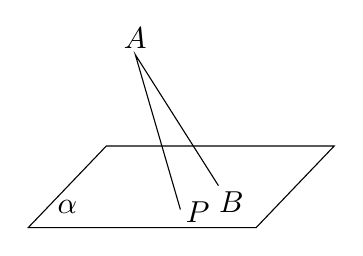
\begin{tikzpicture}[x=1pt, y=1pt,
    every node/.style={inner sep=0pt, font=\fontsize{10.5pt}{12.6pt}\selectfont}]
  \draw[line width=0.398pt] (54.9929,6.5198)   -- (38.6929,62.5048)   -- (68.7409,15.1658);
  \draw[line width=0.398pt] (0.0000,0.0000)   -- (82.3470,0.0000)   -- (110.5530,29.4810)   -- (28.2050,29.4810)   -- cycle;

  \node[anchor=center] at (38.700,68.512) {$A$};  % 源中心 (578.70,536.99)
  \node[anchor=center] at (61.250,5.562) {$P$};  % 源中心 (601.25,474.04)
  \node[anchor=center] at (73.400,9.262) {$B$};  % 源中心 (613.40,477.74)
  \node[anchor=center] at (14.150,7.362) {$\alpha$};  % 源中心 (554.15,475.84)

\end{tikzpicture}
%
% 【自验结果】
%   探针：latexmk -pdfxe（待跑）。
\end{center}
\nopagebreak[4]
(A) 直线　(B) 抛物线　(C) 椭圆　(D) 双曲线的一支

\Needspace{4\baselineskip}
\textbf{解析}

设 \(A\) 在平面 \(\alpha\) 上的射影为 \(H\)，则 \(AB\) 与 \(\alpha\) 所成角为 \(\angle ABH=60^\circ\)，且 \(AH\perp\alpha\)。

在平面 \(\alpha\) 内，动点 \(P\) 满足 \(\angle PAB=30^\circ\)。以 \(AB\) 为轴、半顶角 \(30^\circ\) 的圆锥面与平面 \(\alpha\) 相交：圆锥轴线 \(AB\) 与平面 \(\alpha\) 的夹角为 \(60^\circ\)，而母线与轴线的夹角为 \(30^\circ\)。由于 \(60^\circ>30^\circ\)，截面与圆锥的每条母线都相交，截线为椭圆。

故选 (C)。

（验证：若截面与轴夹角等于半顶角，截线为抛物线；小于则双曲线；此处 \(60^\circ>30^\circ\)，故为椭圆。）

\gkanswer{答案：C}

\end{answer}
\begin{answer}
\gksolhead{8}{绝对值与三角}

\textbf{题目}：

设实数 \(a\)，\(b\)，\(t\) 满足 \(|a+1|=|\sin b|=t\)。则下列说法中正确的是（　）

(A) 若 \(t\) 确定，则 \(b^2\) 唯一确定　(B) 若 \(t\) 确定，则 \(a^2+2a\) 唯一确定　(C) 若 \(t\) 确定，则 \(\sin\dfrac{b}{2}\) 唯一确定　(D) 若 \(t\) 确定，则 \(a^2+a\) 唯一确定

\Needspace{4\baselineskip}
\textbf{解析}

\Needspace{5\baselineskip}
由 \(|a+1|=t\) 得 \(a+1=\pm t\)，故
\nopagebreak[4]
\[
a^2+2a=(a+1)^2-1=t^2-1,
\]
当 \(t\) 确定时，\(a^2+2a\) 唯一确定，(B) 正确。

其余选项：\(a=\pm t-1\)，\(a^2\) 与 \(a^2+a\) 都随 \(a\) 的符号变化，不唯一；\(|\sin b|=t\) 给出 \(\sin b=\pm t\)，\(\sin\dfrac{b}2\) 也不唯一。

故选 (B)。

（验证：取 \(t=\dfrac12\)，由 \(|a+1|=\dfrac12\) 得 \(a=-\dfrac12\) 或 \(a=-\dfrac32\)，此时 \(a^2=\dfrac14\) 或 \(\dfrac94\)、\(a^2+a=-\dfrac14\) 或 \(\dfrac34\)，均不唯一；而 \(a^2+2a=t^2-1=-\dfrac34\) 唯一确定，故选 (B)。）

\gkanswer{答案：B}

\end{answer}
\begin{answer}
\gksolhead{9}{对数运算}

\textbf{题目}：

计算 \(\log_2\dfrac{\sqrt{2}}{2}=\)\gkblank{}，\(2^{\log_2 3+\log_4 3}=\)\gkblank{}。

\Needspace{4\baselineskip}
\textbf{解析}

\nopagebreak[4]
\[
\log_2\frac{\sqrt2}{2}=\log_2 2^{-1/2}=-\frac12.
\]
\Needspace{5\baselineskip}
又
\nopagebreak[4]
\[
2^{\log_2 3+\log_4 3}=2^{\log_2 3}\cdot2^{\log_4 3}
=3\cdot2^{\frac12\log_2 3}
=3\sqrt3.
\]

（验证：\(2^{-1/2}=\dfrac{\sqrt2}{2}\)；\(2^{\log_4 3}=2^{\frac12\log_2 3}=\sqrt3\)。）

\gkanswer{答案：\(-\dfrac12\)；\(3\sqrt3\)}

\end{answer}
\begin{answer}
\gksolhead{10}{等差数列与等比中项}

\textbf{题目}：

已知 \(\{a_n\}\) 是等差数列，公差 \(d\) 不为零。若 \(a_2\)，\(a_3\)，\(a_7\) 成等比数列，且 \(2a_1+a_2=1\)，则 \(a_1=\)\gkblank{}，\(d=\)\gkblank{}。

\Needspace{4\baselineskip}
\textbf{解析}

\Needspace{5\baselineskip}
设 \(a_n=a_1+(n-1)d\)。由 \(a_2\)，\(a_3\)，\(a_7\) 成等比数列，
\nopagebreak[4]
\[
(a_1+2d)^2=(a_1+d)(a_1+6d).
\]
\Needspace{5\baselineskip}
展开整理：
\nopagebreak[4]
\[
a_1^2+4a_1d+4d^2=a_1^2+7a_1d+6d^2
\ \Longrightarrow\ d(3a_1+2d)=0.
\]
\Needspace{5\baselineskip}
因 \(d\neq0\)，故 \(a_1=-\dfrac{2d}{3}\)。又 \(2a_1+a_2=1\)，即 \(3a_1+d=1\)，代入得
\nopagebreak[4]
\[
-2d+d=1\ \Longrightarrow\ d=-1,\qquad a_1=\frac23.
\]

（验证：\(a_2=\dfrac23-1=-\dfrac13\)，\(a_3=-\dfrac43\)，\(a_7=-\dfrac{16}{3}\)；\(a_3^2=\dfrac{16}{9}=a_2a_7=\dfrac{16}{9}\)，成等比。）

\gkanswer{答案：\(a_1=\dfrac23\)，\(d=-1\)}

\end{answer}
\begin{answer}
\gksolhead{11}{三角恒等变换}

\textbf{题目}：

函数 \(f(x)=\sin^2x+\sin x\cos x+1\) 的最小正周期是\gkblank{}，最小值是\gkblank{}。

\Needspace{4\baselineskip}
\textbf{解析}

\nopagebreak[4]
\[
f(x)=\sin^2x+\sin x\cos x+1
=\frac{1-\cos2x}{2}+\frac{\sin2x}{2}+1
=\frac32+\frac{\sqrt2}{2}\sin\left(2x-\frac{\pi}{4}\right).
\]
\Needspace{5\baselineskip}
故最小正周期
\nopagebreak[4]
\[
T=\frac{2\pi}{2}=\pi,
\]
\Needspace{5\baselineskip}
最小值
\nopagebreak[4]
\[
f_{\min}=\frac32-\frac{\sqrt2}{2}=\frac{3-\sqrt2}{2}.
\]

（验证：\(\sin\left(2x-\dfrac{\pi}{4}\right)=-1\) 时取最小值，此时 \(2x-\dfrac{\pi}{4}=-\dfrac{\pi}{2}+2k\pi\)，有解。）

\gkanswer{答案：\(\pi\)；\(\dfrac{3-\sqrt2}{2}\)}

\end{answer}
\begin{answer}
\gksolhead{12}{分段函数}

\textbf{题目}：

\Needspace{5\baselineskip}
已知函数
\nopagebreak[4]
\[
f(x)=\begin{cases}
x^2, & x\leqslant1,\\
x+\dfrac{6}{x}-6, & x>1,
\end{cases}
\]
则 \(f(f(-2))=\)\gkblank{}，\(f(x)\) 的最小值是\gkblank{}。

\Needspace{4\baselineskip}
\textbf{解析}

\Needspace{5\baselineskip}
\(f(-2)=(-2)^2=4\)，故
\nopagebreak[4]
\[
f(f(-2))=f(4)=4+\frac64-6=-\frac12.
\]
当 \(x\leqslant1\) 时，\(f(x)=x^2\geqslant0\)，最小值为 \(0\)（在 \(x=0\) 处）。

\Needspace{5\baselineskip}
当 \(x>1\) 时，
\nopagebreak[4]
\[
f(x)=x+\frac6x-6\geqslant2\sqrt6-6,
\]
\Needspace{5\baselineskip}
等号在 \(x=\sqrt6>1\) 处成立。由于 \(2\sqrt6-6\approx-1.10<0\)，故
\nopagebreak[4]
\[
f_{\min}=2\sqrt6-6.
\]

（验证：\(x=\sqrt6\) 在 \(x>1\) 范围内，等号可取；\(x\leqslant1\) 段的最小值 \(0\) 大于 \(2\sqrt6-6\)，故全局最小值为 \(2\sqrt6-6\)。）

\gkanswer{答案：\(-\dfrac12\)；\(2\sqrt6-6\)}

\end{answer}
\begin{answer}
\gksolhead{13}{平面向量}

\textbf{题目}：

已知 \(\boldsymbol{e}_1\)，\(\boldsymbol{e}_2\) 是平面单位向量，且 \(\boldsymbol{e}_1\cdot\boldsymbol{e}_2=\dfrac{1}{2}\)。若平面向量 \(\boldsymbol{b}\) 满足 \(\boldsymbol{b}\cdot\boldsymbol{e}_1=\boldsymbol{b}\cdot\boldsymbol{e}_2=1\)，则 \(|\boldsymbol{b}|=\)\gkblank{}。

\Needspace{4\baselineskip}
\textbf{解析}

\Needspace{5\baselineskip}
由 \(\boldsymbol{e}_1\cdot\boldsymbol{e}_2=\dfrac12\)，且 \(|\boldsymbol{e}_1|=|\boldsymbol{e}_2|=1\)。设
\nopagebreak[4]
\[
\boldsymbol{b}=x\boldsymbol{e}_1+y\boldsymbol{e}_2.
\]
\Needspace{5\baselineskip}
则
\nopagebreak[4]
\[
\boldsymbol{b}\cdot\boldsymbol{e}_1=x+\frac{y}2=1,\qquad
\boldsymbol{b}\cdot\boldsymbol{e}_2=\frac{x}2+y=1.
\]
\Needspace{5\baselineskip}
两式相减得 \(\dfrac{x-y}{2}=0\)，故 \(x=y\)；代入得 \(\dfrac{3x}{2}=1\)，即 \(x=y=\dfrac23\)。于是
\nopagebreak[4]
\[
|\boldsymbol{b}|^2=x^2+y^2+2xy\cdot\frac12
=\frac49+\frac49+\frac49=\frac43,
\]
\Needspace{5\baselineskip}
故
\nopagebreak[4]
\[
|\boldsymbol{b}|=\frac{2}{\sqrt3}=\frac{2\sqrt3}{3}.
\]

（验证：把 \(\boldsymbol{b}=\dfrac23(\boldsymbol{e}_1+\boldsymbol{e}_2)\) 代回，两个点积均为 \(\dfrac23+\dfrac13=1\)，满足条件。）

\gkanswer{答案：\(\dfrac{2\sqrt3}{3}\)}

\end{answer}
\begin{answer}
\gksolhead{14}{绝对值与最值}

\textbf{题目}：

已知实数 \(x\)，\(y\) 满足 \(x^2+y^2\leqslant1\)，则 \(|2x+y-4|+|6-x-3y|\) 的最大值是\gkblank{}。

\Needspace{4\baselineskip}
\textbf{解析}

\Needspace{5\baselineskip}
由 \(x^2+y^2\leqslant1\) 得
\nopagebreak[4]
\[
2x+y\leqslant\sqrt{2^2+1^2}=\sqrt5<4,
\]
故 \(2x+y-4<0\)，\(|2x+y-4|=4-2x-y\)。

\Needspace{5\baselineskip}
又
\nopagebreak[4]
\[
x+3y\leqslant\sqrt{1+9}=\sqrt{10}<6,
\]
故 \(6-x-3y>0\)，\(|6-x-3y|=6-x-3y\)。

\Needspace{5\baselineskip}
于是
\nopagebreak[4]
\[
|2x+y-4|+|6-x-3y|=10-3x-4y.
\]
\Needspace{5\baselineskip}
由柯西不等式，
\nopagebreak[4]
\[
3x+4y\geqslant-\sqrt{(3^2+4^2)(x^2+y^2)}\geqslant-5,
\]
\Needspace{5\baselineskip}
等号在 \((x,y)=\left(-\dfrac35,-\dfrac45\right)\) 处成立。故最大值为
\nopagebreak[4]
\[
10+5=15.
\]

（验证：取 \((x,y)=\left(-\dfrac35,-\dfrac45\right)\)，\(x^2+y^2=1\)，原式 \(=\left|-\dfrac65-\dfrac45-4\right|+\left|6+\dfrac35+\dfrac{12}{5}\right|=6+9=15\)。）

\gkanswer{答案：\(15\)}

\end{answer}
\begin{answer}
\gksolhead{15}{椭圆的离心率}

\textbf{题目}：

椭圆 \(\dfrac{x^2}{a^2}+\dfrac{y^2}{b^2}=1\)（\(a>b>0\)）的右焦点 \(F(c,0)\) 关于直线 \(y=\dfrac{b}{c}x\) 的对称点 \(Q\) 在椭圆上，则椭圆的离心率是\gkblank{}。

\Needspace{4\baselineskip}
\textbf{解析}

\Needspace{5\baselineskip}
直线 \(y=\dfrac{b}c x\) 过原点，方向向量为 \((c,b)\)。点 \(F(c,0)\) 关于该直线的对称点为
\nopagebreak[4]
\[
Q=2\frac{(c,0)\cdot(c,b)}{c^2+b^2}(c,b)-(c,0).
\]
\Needspace{5\baselineskip}
由 \(c^2+b^2=a^2\)，得
\nopagebreak[4]
\[
Q=\left(\frac{2c^3}{a^2}-c,\ \frac{2c^2b}{a^2}\right)
=\left(\frac{c(a^2-2b^2)}{a^2},\ \frac{2c^2b}{a^2}\right).
\]
\Needspace{5\baselineskip}
令 \(e=\dfrac{c}a\)，则 \(b^2=a^2(1-e^2)\)，于是
\nopagebreak[4]
\[
\frac{x_Q}{a}=e(2e^2-1),\qquad \frac{y_Q}{b}=2e^2.
\]
\Needspace{5\baselineskip}
由 \(Q\) 在椭圆上，
\nopagebreak[4]
\[
e^2(2e^2-1)^2+4e^4=1.
\]
\Needspace{5\baselineskip}
令 \(u=e^2\)，化简得
\nopagebreak[4]
\[
4u^3+u-1=0
\ \Longrightarrow\ \left(u-\frac12\right)(4u^2+2u+2)=0.
\]
\Needspace{5\baselineskip}
二次因子无实根，故 \(u=\dfrac12\)，即
\nopagebreak[4]
\[
e=\frac{\sqrt2}{2}.
\]

（验证：\(e=\dfrac{\sqrt2}{2}\) 时 \(b=c\)，直线 \(y=x\)，\(F(c,0)\) 的对称点为 \((0,c)\)，代入椭圆 \(\dfrac{0}{2c^2}+\dfrac{c^2}{c^2}=1\)，成立。）

\gkanswer{答案：\(\dfrac{\sqrt2}{2}\)}

\end{answer}
\begin{answer}
\gksolhead{16}{解三角形}

\textbf{题目}：

在 \(\triangle ABC\) 中，内角 \(A\)，\(B\)，\(C\) 所对的边分别为 \(a\)，\(b\)，\(c\)。已知 \(\tan\left(\dfrac{\pi}{4}+A\right)=2\)。

（1） 求 \(\dfrac{\sin 2A}{\sin 2A+\cos^2A}\) 的值；

（2） 若 \(B=\dfrac{\pi}{4}\)，\(a=3\)，求 \(\triangle ABC\) 的面积。

\Needspace{4\baselineskip}
\textbf{解析}

\gksubpart{(1)}

\Needspace{5\baselineskip}
由 \(\tan\left(\dfrac{\pi}{4}+A\right)=2\) 及两角和的正切公式，
\nopagebreak[4]
\[
\frac{1+\tan A}{1-\tan A}=2
\ \Longrightarrow\ 1+\tan A=2-2\tan A
\ \Longrightarrow\ \tan A=\frac13.
\]
\Needspace{5\baselineskip}
将所求式分子分母同除以 \(\cos^2A\)：
\nopagebreak[4]
\[
\frac{\sin2A}{\sin2A+\cos^2A}
=\frac{2\tan A}{2\tan A+1}
=\frac{2/3}{2/3+1}
=\frac25.
\]

\gksubpart{(2)}

\Needspace{5\baselineskip}
由 \(\tan A=\dfrac13\) 且 \(A\) 为三角形内角，得
\nopagebreak[4]
\[
\sin A=\frac{1}{\sqrt{10}},\qquad \cos A=\frac{3}{\sqrt{10}}.
\]
\Needspace{5\baselineskip}
又 \(B=\dfrac{\pi}{4}\)，故
\nopagebreak[4]
\[
\sin C=\sin\left(\frac{3\pi}{4}-A\right)
=\frac{\sqrt2}{2}(\cos A+\sin A)
=\frac{\sqrt2}{2}\cdot\frac{4}{\sqrt{10}}
=\frac{2\sqrt5}{5}.
\]
\Needspace{5\baselineskip}
由正弦定理，
\nopagebreak[4]
\[
b=\frac{a\sin B}{\sin A}
=\frac{3\cdot\frac{\sqrt2}{2}}{\frac{1}{\sqrt{10}}}
=3\sqrt5.
\]
\Needspace{5\baselineskip}
故
\nopagebreak[4]
\[
S_{\triangle ABC}=\frac12ab\sin C
=\frac12\cdot3\cdot3\sqrt5\cdot\frac{2\sqrt5}{5}=9.
\]

（验证：\(C=\pi-A-B\)，\(\sin C>0\)；面积 \(9\) 与 \(a=3\)、\(b=3\sqrt5\)、\(\sin C=\dfrac{2\sqrt5}{5}\) 的乘积一致。）

\gkanswer{答案（1）：\(\dfrac25\)。}

\gkanswer{答案（2）：\(9\)。}

\end{answer}
\begin{answer}
\gksolhead{17}{数列}

\textbf{题目}：

已知数列 \(\{a_n\}\) 和 \(\{b_n\}\) 满足 \(a_1=2\)，\(b_1=1\)，\(a_{n+1}=2a_n\)（\(n\in\mathbf{N}^*\)），\(b_1+\dfrac{1}{2}b_2+\dfrac{1}{3}b_3+\cdots+\dfrac{1}{n}b_n=b_{n+1}-1\)（\(n\in\mathbf{N}^*\)）。

（1） 求 \(a_n\) 与 \(b_n\)；

（2） 记数列 \(\{a_nb_n\}\) 的前 \(n\) 项和为 \(T_n\)，求 \(T_n\)。

\Needspace{4\baselineskip}
\textbf{解析}

\gksubpart{(1)}

\Needspace{5\baselineskip}
由 \(a_{n+1}=2a_n\)，\(a_1=2\)，得
\nopagebreak[4]
\[
a_n=2^n.
\]
\Needspace{5\baselineskip}
对于 \(\{b_n\}\)，当 \(n=1\) 时 \(b_1=b_2-1\)，故 \(b_2=2\)。当 \(n\geqslant2\) 时，两式
\nopagebreak[4]
\[
b_1+\frac12b_2+\cdots+\frac1n b_n=b_{n+1}-1,
\]
\nopagebreak[4]
\[
b_1+\frac12b_2+\cdots+\frac1{n-1}b_{n-1}=b_n-1
\]
\Needspace{5\baselineskip}
相减得
\nopagebreak[4]
\[
\frac{b_n}{n}=b_{n+1}-b_n
\ \Longrightarrow\ b_{n+1}=\frac{n+1}{n}b_n.
\]
\Needspace{5\baselineskip}
故 \(\dfrac{b_n}{n}\) 为常数列，\(\dfrac{b_n}{n}=\dfrac{b_1}{1}=1\)，即
\nopagebreak[4]
\[
b_n=n.
\]

\gksubpart{(2)}

\nopagebreak[4]
\[
a_nb_n=n\cdot2^n.
\]
\Needspace{5\baselineskip}
设
\nopagebreak[4]
\[
T_n=\sum_{k=1}^{n}k2^k.
\]
\Needspace{5\baselineskip}
则
\nopagebreak[4]
\[
2T_n=\sum_{k=1}^{n}k2^{k+1}.
\]
\Needspace{5\baselineskip}
两式相减：
\nopagebreak[4]
\[
2T_n-T_n
=\left(2^2+2\cdot2^3+\cdots+(n-1)2^n+n2^{n+1}\right)
-\left(2+2\cdot2^2+\cdots+n2^n\right),
\]
\Needspace{5\baselineskip}
即
\nopagebreak[4]
\[
T_n=-2-2^2-2^3-\cdots-2^n+n2^{n+1}
=-\left(2^{n+1}-2\right)+n2^{n+1}.
\]
\Needspace{5\baselineskip}
故
\nopagebreak[4]
\[
T_n=(n-1)2^{n+1}+2.
\]

（验证：\(n=1\) 时 \(T_1=2\)，公式给 \((0)\cdot4+2=2\)；\(n=2\) 时 \(T_2=2+8=10\)，公式给 \(1\cdot8+2=10\)。）

\gkanswer{答案（1）：\(a_n=2^n\)，\(b_n=n\)。}

\gkanswer{答案（2）：\(T_n=(n-1)2^{n+1}+2\)。}

\end{answer}
\begin{answer}
\gksolhead{18}{立体几何}

\textbf{题目}：

如图，在三棱柱 \(ABC-A_1B_1C_1\) 中，\(\angle BAC=90^\circ\)，\(AB=AC=2\)，\(AA_1=4\)，\(A_1\) 在底面 \(ABC\) 的射影为 \(BC\) 的中点，\(D\) 是 \(B_1C_1\) 的中点。

（1） 证明：\(A_1D\perp\) 平面 \(A_1BC\)；

（2） 求直线 \(A_1B\) 和平面 \(BB_1C_1C\) 所成的角的正弦值。
\nopagebreak[4]
\begin{center}% f2015zjw_q18_prism.tex — 2015 年高考数学·浙江卷·文科 第 18 题（三棱柱）
%
% 【来源】`.work/phase3-b18/source/2015浙江文.pdf`（SHA-256
%   a0e49283fb3d086029ec3c96de7e96cc6118365378ea0a24273c6f58285ec977），
%   第 2 页（合订本页 992）；内容对象 23。逐路径实测见
%   `.work/phase3-b18/figure-inventory.md`。
%
% 【坐标口径】源 PDF 用户空间（原点左下、y 向上）。本图本地坐标
%   (x, y) = (x_page − 259.718, y_page − 562.833)，1 单位 = 1 TeX pt。
%   路径坐标逐点照录内容流（含三次贝塞尔控制点）。
%
% 元素计数：12 条路径（8 实＋4 虚）＋7 个标签
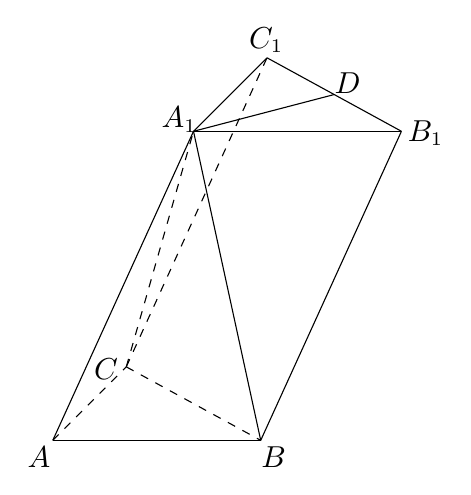
\begin{tikzpicture}[x=1pt, y=1pt,
    every node/.style={inner sep=0pt, font=\fontsize{10.5pt}{12.6pt}\selectfont}]
  \draw[line width=0.3985pt] (0.0000,0.0000)   (0.0000,0.0000)   -- (75.1352,0.0000);
  \draw[line width=0.3985pt] (75.1352,0.0000)   (75.1352,0.0000)   -- (50.8477,111.6752);
  \draw[line width=0.3985pt] (50.8477,111.6752)   (50.8477,111.6752)   -- (125.9829,111.6752);
  \draw[line width=0.3985pt] (125.9829,111.6752)   (125.9829,111.6752)   -- (77.4080,138.2355);
  \draw[line width=0.3985pt] (77.4080,138.2355)   (77.4080,138.2355)   -- (50.8477,111.6752);
  \draw[line width=0.3985pt] (75.1352,0.0000)   (75.1352,0.0000)   -- (125.9829,111.6752);
  \draw[line width=0.3985pt] (0.0000,0.0000)   (0.0000,0.0000)   -- (50.8477,111.6752);
  \draw[line width=0.3985pt] (101.6955,124.9553)   (101.6955,124.9553)   -- (50.8477,111.6752);
  \draw[line width=0.3985pt, dash pattern=on 2.98883pt off 2.98883pt, dash phase=0.0pt] (0.0000,0.0000)   (0.0000,0.0000)   -- (26.5603,26.5603);
  \draw[line width=0.3985pt, dash pattern=on 2.98883pt off 2.98883pt, dash phase=0.0pt] (26.5603,26.5603)   (26.5603,26.5603)   -- (77.4080,138.2355);
  \draw[line width=0.3985pt, dash pattern=on 2.98883pt off 2.98883pt, dash phase=0.0pt] (26.5603,26.5603)   (26.5603,26.5603)   -- (50.8477,111.6752);
  \draw[line width=0.3985pt, dash pattern=on 2.98883pt off 2.98883pt, dash phase=0.0pt] (26.5603,26.5603)   (26.5603,26.5603)   -- (75.1352,0.0000);

  \node[anchor=center] at (45.682,115.957) {$A_1$};  % 源中心 (305.40,678.79)
  \node[anchor=center] at (134.682,111.057) {$B_1$};  % 源中心 (394.40,673.89)
  \node[anchor=center] at (77.132,144.557) {$C_1$};  % 源中心 (336.85,707.39)
  \node[anchor=center] at (106.482,128.907) {$D$};  % 源中心 (366.20,691.74)
  \node[anchor=center] at (19.232,25.607) {$C$};  % 源中心 (278.95,588.44)
  \node[anchor=center] at (-4.968,-5.893) {$A$};  % 源中心 (254.75,556.94)
  \node[anchor=center] at (79.782,-5.893) {$B$};  % 源中心 (339.50,556.94)

\end{tikzpicture}
%
% 【自验结果】
%   探针：latexmk -pdfxe（待跑）。
\end{center}
\nopagebreak[4]
\Needspace{4\baselineskip}
\textbf{解析}

\gksubpart{(1)}

取 \(BC\) 的中点 \(M\)。由 \(AB=AC\)，\(M\) 为 \(BC\) 中点，故 \(AM\perp BC\)。又 \(A_1\) 在底面的射影为 \(M\)，故 \(A_1M\perp\) 平面 \(ABC\)。

\Needspace{5\baselineskip}
以 \(M\) 为原点，\(MB\) 为 \(x\) 轴，\(MA\) 为 \(y\) 轴，\(MA_1\) 为 \(z\) 轴建立空间直角坐标系。由 \(AB=AC=2\)，\(\angle BAC=90^\circ\)，得 \(BC=2\sqrt2\)，故
\nopagebreak[4]
\[
B(\sqrt2,0,0),\quad C(-\sqrt2,0,0),\quad A(0,\sqrt2,0).
\]
\Needspace{5\baselineskip}
由 \(AA_1=4\)，\(A_1M=\sqrt{4^2-(\sqrt2)^2}=\sqrt{14}\)，故
\nopagebreak[4]
\[
A_1(0,0,\sqrt{14}).
\]
\Needspace{5\baselineskip}
于是
\nopagebreak[4]
\[
B_1=B+\overrightarrow{AA_1}=(\sqrt2,-\sqrt2,\sqrt{14}),\qquad
C_1=(-\sqrt2,-\sqrt2,\sqrt{14}),
\]
\nopagebreak[4]
\[
D=\left(0,-\sqrt2,\sqrt{14}\right).
\]
\Needspace{5\baselineskip}
故
\nopagebreak[4]
\[
\overrightarrow{A_1D}=(0,-\sqrt2,0).
\]
\Needspace{5\baselineskip}
平面 \(A_1BC\) 中，\(\overrightarrow{BC}=(-2\sqrt2,0,0)\)，\(\overrightarrow{BA_1}=(-\sqrt2,0,\sqrt{14})\)，法向量可取
\nopagebreak[4]
\[
\boldsymbol{n}=\overrightarrow{BC}\times\overrightarrow{BA_1}=(0,4\sqrt7,0)\parallel(0,1,0).
\]
因 \(\overrightarrow{A_1D}\parallel\boldsymbol{n}\)，故 \(A_1D\perp\) 平面 \(A_1BC\)。

\gksubpart{(2)}

\Needspace{5\baselineskip}
平面 \(BB_1C_1C\) 中，
\nopagebreak[4]
\[
\overrightarrow{BC}=(-2\sqrt2,0,0),\qquad
\overrightarrow{BB_1}=(0,-\sqrt2,\sqrt{14}).
\]
\Needspace{5\baselineskip}
法向量
\nopagebreak[4]
\[
\boldsymbol{n}_2=\overrightarrow{BC}\times\overrightarrow{BB_1}
=(0,4\sqrt7,4).
\]
\Needspace{5\baselineskip}
又
\nopagebreak[4]
\[
\overrightarrow{A_1B}=(\sqrt2,0,-\sqrt{14}),\qquad |\overrightarrow{A_1B}|=4.
\]
\Needspace{5\baselineskip}
设直线 \(A_1B\) 与平面 \(BB_1C_1C\) 所成角为 \(\theta\)，则
\nopagebreak[4]
\[
\sin\theta
=\frac{|\overrightarrow{A_1B}\cdot\boldsymbol{n}_2|}{|\overrightarrow{A_1B}||\boldsymbol{n}_2|}
=\frac{4\sqrt{14}}{4\cdot8\sqrt2}
=\frac{\sqrt7}{8}.
\]

（验证：\(|\boldsymbol{n}_2|=\sqrt{112+16}=8\sqrt2\)，点积 \(\overrightarrow{A_1B}\cdot\boldsymbol{n}_2=(-\sqrt{14})\cdot4=-4\sqrt{14}\)，取绝对值后结果 \(\dfrac{\sqrt7}{8}<1\)。）

\gkanswer{答案（1）：成立（建系得 \(\overrightarrow{A_1D}\) 与平面 \(A_1BC\) 的法向量平行）。}

\gkanswer{答案（2）：\(\dfrac{\sqrt7}{8}\)。}

\end{answer}
\begin{answer}
\gksolhead{19}{抛物线与圆}

\textbf{题目}：

如图，已知抛物线 \(C_1\)：\(y=\dfrac{1}{4}x^2\)，圆 \(C_2\)：\(x^2+(y-1)^2=1\)，过点 \(P(t,0)\)（\(t>0\)）作不过原点 \(O\) 的直线 \(PA\)，\(PB\) 分别与抛物线 \(C_1\) 和圆 \(C_2\) 相切，\(A\)，\(B\) 为切点。

（1） 求点 \(A\)，\(B\) 的坐标；

（2） 求 \(\triangle PAB\) 的面积。

注：直线与抛物线有且只有一个公共点，且与抛物线的对称轴不平行，则称该直线与抛物线相切，称该公共点为切点。
\nopagebreak[4]
\begin{center}% f2015zjw_q19_conic.tex — 2015 年高考数学·浙江卷·文科 第 19 题（抛物线与圆）
%
% 【来源】`.work/phase3-b18/source/2015浙江文.pdf`（SHA-256
%   a0e49283fb3d086029ec3c96de7e96cc6118365378ea0a24273c6f58285ec977），
%   第 2 页（合订本页 992）；内容对象 23。逐路径实测见
%   `.work/phase3-b18/figure-inventory.md`。
%
% 【坐标口径】源 PDF 用户空间（原点左下、y 向上）。本图本地坐标
%   (x, y) = (x_page − 571.28, y_page − 576.775)，1 单位 = 1 TeX pt。
%   路径坐标逐点照录内容流（含三次贝塞尔控制点）。
%
% 元素计数：9 条路径（x/y 轴＋箭头、圆、3 直线、抛物线）＋6 个标签
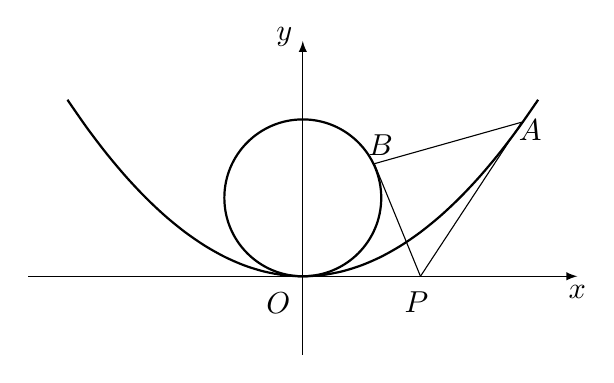
\begin{tikzpicture}[x=1pt, y=1pt,
    every node/.style={inner sep=0pt, font=\fontsize{10.5pt}{12.6pt}\selectfont}]
  \draw[line width=0.3985pt] (0.0002,0.0000)   -- (194.8413,0.0000);
  \fill[line width=0.3985pt] (198.4278,0.0000)   .. controls (197.3651,0.1992) and (195.6383,0.7970) .. (194.4428,1.4944)   -- (194.4428,-1.4944)   .. controls (195.6383,-0.7970) and (197.3651,-0.1993) .. (198.4278,0.0000);
  \draw[line width=0.3985pt] (99.2140,-28.3468)   -- (99.2140,81.4539);
  \fill[line width=0.3985pt] (99.2140,85.0404)   .. controls (99.0148,83.9777) and (98.4170,82.2509) .. (97.7196,81.0554)   -- (100.7084,81.0554)   .. controls (100.0110,82.2509) and (99.4133,83.9777) .. (99.2140,85.0404);
  \draw[line width=0.79701pt] (99.2140,28.3468)   (127.5608,28.3468)   .. controls (127.5608,44.0025) and (114.8697,56.6936) .. (99.2140,56.6936)   .. controls (83.5583,56.6936) and (70.8672,44.0025) .. (70.8672,28.3468)   .. controls (70.8672,12.6911) and (83.5583,0.0000) .. (99.2140,0.0000)   .. controls (114.8697,0.0000) and (127.5608,12.6911) .. (127.5608,28.3468)   -- cycle   (99.2140,28.3468);
  \draw[line width=0.3985pt] (178.3299,55.6871)   -- (125.0495,40.6720);
  \draw[line width=0.3985pt] (141.7342,0.0000)   -- (125.0495,40.6720);
  \draw[line width=0.3985pt] (141.7342,0.0000)   -- (178.3299,55.6871);
  \draw[line width=0.79701pt] (14.1736,63.7803)   .. controls (14.1736,63.7803) and (19.2938,56.2971) .. (21.2603,53.5932)   .. controls (23.2268,50.8892) and (26.3805,46.7500) .. (28.3470,44.2919)   .. controls (30.3135,41.8337) and (33.4672,38.0888) .. (35.4337,35.8764)   .. controls (37.4002,33.6641) and (40.5539,30.3133) .. (42.5204,28.3468)   .. controls (44.4869,26.3803) and (47.6406,23.4237) .. (49.6071,21.7030)   .. controls (51.5736,19.9823) and (54.7273,17.4199) .. (56.6938,15.9451)   .. controls (58.6603,14.4702) and (61.8140,12.3020) .. (63.7805,11.0730)   .. controls (65.7470,9.8439) and (68.9007,8.0699) .. (70.8672,7.0867)   .. controls (72.8337,6.1034) and (75.9874,4.7237) .. (77.9539,3.9863)   .. controls (79.9204,3.2488) and (83.0741,2.2633) .. (85.0406,1.7717)   .. controls (87.0071,1.2800) and (90.1608,0.6887) .. (92.1273,0.4429)   .. controls (94.0938,0.1971) and (97.2475,0.0000) .. (99.2140,0.0000)   .. controls (101.1805,0.0000) and (104.3342,0.1971) .. (106.3007,0.4429)   .. controls (108.2672,0.6887) and (111.4209,1.2800) .. (113.3874,1.7717)   .. controls (115.3539,2.2633) and (118.5076,3.2488) .. (120.4741,3.9863)   .. controls (122.4406,4.7237) and (125.5943,6.1034) .. (127.5608,7.0867)   .. controls (129.5273,8.0699) and (132.6810,9.8439) .. (134.6475,11.0730)   .. controls (136.6140,12.3020) and (139.7677,14.4702) .. (141.7342,15.9451)   .. controls (143.7007,17.4199) and (146.8544,19.9823) .. (148.8209,21.7030)   .. controls (150.7874,23.4237) and (153.9411,26.3803) .. (155.9076,28.3468)   .. controls (157.8741,30.3133) and (161.0278,33.6641) .. (162.9943,35.8764)   .. controls (164.9608,38.0888) and (168.1145,41.8337) .. (170.0810,44.2919)   .. controls (172.0475,46.7500) and (175.2012,50.8892) .. (177.1677,53.5932)   .. controls (179.1342,56.2971) and (184.2544,63.7803) .. (184.2544,63.7803);

  \node[anchor=center] at (92.570,86.415) {$y$};  % 源中心 (663.85,663.19)
  \node[anchor=center] at (181.420,52.865) {$A$};  % 源中心 (752.70,629.64)
  \node[anchor=center] at (127.320,47.215) {$B$};  % 源中心 (698.60,623.99)
  \node[anchor=center] at (90.370,-9.685) {$O$};  % 源中心 (661.65,567.09)
  \node[anchor=center] at (140.320,-9.235) {$P$};  % 源中心 (711.60,567.54)
  \node[anchor=center] at (198.420,-5.585) {$x$};  % 源中心 (769.70,571.19)

\end{tikzpicture}
%
% 【自验结果】
%   探针：latexmk -pdfxe（待跑）。
\end{center}
\nopagebreak[4]
\Needspace{4\baselineskip}
\textbf{解析}

\gksubpart{(1)}

\Needspace{5\baselineskip}
抛物线 \(C_1:y=\dfrac14x^2\) 在点 \(A\left(a,\dfrac{a^2}{4}\right)\) 处的切线为
\nopagebreak[4]
\[
y=\frac{a}2x-\frac{a^2}{4}.
\]
\Needspace{5\baselineskip}
它过 \(P(t,0)\)，故
\nopagebreak[4]
\[
0=\frac{a}2t-\frac{a^2}{4}
\ \Longrightarrow\ a(a-2t)=0.
\]
\Needspace{5\baselineskip}
因 \(PA\) 不过原点且 \(t>0\)，取 \(a=2t\)，故
\nopagebreak[4]
\[
A(2t,t^2).
\]

\Needspace{5\baselineskip}
设过 \(P(t,0)\) 的直线 \(y=k(x-t)\) 与圆 \(C_2:x^2+(y-1)^2=1\) 相切。圆心 \((0,1)\) 到直线的距离为 \(1\)：
\nopagebreak[4]
\[
\frac{|1+kt|}{\sqrt{1+k^2}}=1
\ \Longrightarrow\ (1+kt)^2=1+k^2
\ \Longrightarrow\ k\left(2t+k(t^2-1)\right)=0.
\]
\Needspace{5\baselineskip}
取 \(k=\dfrac{2t}{1-t^2}\)。切点 \(B\) 为圆心到直线的垂足：
\nopagebreak[4]
\[
B=\left(\frac{2t}{1+t^2},\frac{2t^2}{1+t^2}\right).
\]

\gksubpart{(2)}

\nopagebreak[4]
\[
\overrightarrow{PA}=(t,t^2),\qquad
\overrightarrow{PB}=\left(\frac{t(1-t^2)}{1+t^2},\frac{2t^2}{1+t^2}\right).
\]
\Needspace{5\baselineskip}
于是
\nopagebreak[4]
\[
S_{\triangle PAB}
=\frac12\left|\overrightarrow{PA}\times\overrightarrow{PB}\right|
=\frac12\cdot\frac{t^3(1+t^2)}{1+t^2}
=\frac{t^3}{2}.
\]

（验证：叉积 \(t\cdot\dfrac{2t^2}{1+t^2}-t^2\cdot\dfrac{t(1-t^2)}{1+t^2}=\dfrac{t^3(1+t^2)}{1+t^2}=t^3\)，面积 \(t^3/2\)。）

\gkanswer{答案（1）：\(A(2t,t^2)\)，\(B\left(\dfrac{2t}{1+t^2},\dfrac{2t^2}{1+t^2}\right)\)。}

\gkanswer{答案（2）：\(S=\dfrac{t^3}{2}\)。}

\end{answer}
\begin{answer}
\gksolhead{20}{二次函数}

\textbf{题目}：

设函数 \(f(x)=x^2+ax+b\)（\(a,b\in\mathbf{R}\)）。

（1） 当 \(b=\dfrac{a^2}{4}+1\) 时，求函数 \(f(x)\) 在 \([-1,1]\) 上的最小值 \(g(a)\) 的表达式；

（2） 已知函数 \(f(x)\) 在 \([-1,1]\) 上存在零点，\(0\leqslant b-2a\leqslant1\)，求 \(b\) 的取值范围。

\Needspace{4\baselineskip}
\textbf{解析}

\gksubpart{(1)}

\Needspace{5\baselineskip}
当 \(b=\dfrac{a^2}{4}+1\) 时，
\nopagebreak[4]
\[
f(x)=x^2+ax+\frac{a^2}{4}+1=\left(x+\frac{a}2\right)^2+1.
\]
对称轴为 \(x=-\dfrac{a}2\)。

\begin{itemize}
\item 若 \(-\dfrac{a}2\leqslant-1\)，即 \(a\geqslant2\)，则 \(f\) 在 \([-1,1]\) 上递增，最小值
\end{itemize}
\nopagebreak[4]
  \[
  g(a)=f(-1)=\frac{a^2}{4}-a+2.
  \]
\begin{itemize}
\item 若 \(-1<-\dfrac{a}2<1\)，即 \(-2<a<2\)，则顶点在区间内，最小值
\end{itemize}
\nopagebreak[4]
  \[
  g(a)=1.
  \]
\begin{itemize}
\item 若 \(-\dfrac{a}2\geqslant1\)，即 \(a\leqslant-2\)，则 \(f\) 在 \([-1,1]\) 上递减，最小值
\end{itemize}
\nopagebreak[4]
  \[
  g(a)=f(1)=\frac{a^2}{4}+a+2.
  \]

\Needspace{5\baselineskip}
故
\nopagebreak[4]
\[
g(a)=\begin{cases}
\dfrac{a^2}{4}+a+2, & a\leqslant-2,\\
1, & -2<a<2,\\
\dfrac{a^2}{4}-a+2, & a\geqslant2.
\end{cases}
\]

\gksubpart{(2)}

\Needspace{5\baselineskip}
设 \(x_0\in[-1,1]\) 是 \(f\) 的零点。若 \(x_0=0\)，则 \(b=0\)；若 \(x_0\neq0\)，则
\nopagebreak[4]
\[
a=-\frac{x_0^2+b}{x_0}.
\]
\Needspace{5\baselineskip}
记 \(c=b-2a\in[0,1]\)，则
\nopagebreak[4]
\[
c=b-2a=b+2\cdot\frac{x_0^2+b}{x_0}
=b\left(1+\frac2{x_0}\right)+2x_0,
\]
\Needspace{5\baselineskip}
故
\nopagebreak[4]
\[
b\left(1+\frac2{x_0}\right)=c-2x_0,
\]
\Needspace{5\baselineskip}
即
\nopagebreak[4]
\[
b=\frac{x_0(c-2x_0)}{x_0+2}.
\]

\Needspace{5\baselineskip}
对固定 \(x_0\)，\(b\) 关于 \(c\in[0,1]\) 线性，端点值为
\nopagebreak[4]
\[
b_0=-\frac{2x_0^2}{x_0+2},\qquad
b_1=\frac{x_0(1-2x_0)}{x_0+2}.
\]

\Needspace{5\baselineskip}
当 \(x_0\in(0,1]\) 时，\(b_1\) 的最大值在 \(x_0=\sqrt5-2\) 处取得，为
\nopagebreak[4]
\[
9-4\sqrt5;
\]
\Needspace{5\baselineskip}
\(b_0\) 的最小值为 \(-\dfrac23\)。故这一段给出
\nopagebreak[4]
\[
b\in\left[-\frac23,\,9-4\sqrt5\right].
\]

\Needspace{5\baselineskip}
当 \(x_0\in[-1,0)\) 时，\(b_1\) 在 \(x_0=-1\) 处取最小值 \(-3\)，在 \(x_0\to0^-\) 时趋于 \(0\)；\(b_0\) 在 \([-1,0)\) 上的值域为 \([-2,0)\)。合并得
\nopagebreak[4]
\[
b\in[-3,0).
\]
\Needspace{5\baselineskip}
再并入 \(x_0=0\) 时的 \(b=0\)，得
\nopagebreak[4]
\[
b\in[-3,0]\cup\left[-\frac23,9-4\sqrt5\right]
=[-3,\,9-4\sqrt5].
\]

（验证：取 \(x_0=-1,c=1\) 得 \(b=-3\)，端点可取；取 \(x_0=\sqrt5-2\)、\(c=1\) 得 \(b=9-4\sqrt5\)，端点可取；区间内各值由连续性与线性插值覆盖。）

\gkanswer{答案（1）：$g(a)=\begin{cases}\dfrac{a^2}{4}+a+2,&a\leqslant-2,\\1,&-2<a<2,\\\dfrac{a^2}{4}-a+2,&a\geqslant2.\end{cases}$}

\gkanswer{答案（2）：\(b\in[-3,\,9-4\sqrt5]\)。}

\end{answer}